\documentclass[12pt,oneside,a4paper]{report}
%-------------------------------------------------------
% PACKAGES

\usepackage{natbib}
\usepackage{amsmath}
\usepackage{graphicx}

% COMANDS FOR TABLE
\usepackage{dcolumn}
\usepackage{caption}
\newcommand\fnote[1]{\captionsetup{font=scriptsize, format=hang}\caption*{#1}}
\usepackage{float}                 % to force position of figures and tables
\usepackage{fancyref}			   % to cross-referencing
\usepackage{blindtext}			   % to create bullet lists
\usepackage{enumitem}   		   % to enumerate lists
\usepackage{multirow}			   % to create multirow and multicolumn tables
\usepackage{booktabs} 			   % to format tables
\usepackage{caption}			   % to use subfigures
\usepackage{subcaption}
\usepackage{pdflscape}			   % to rotate elements
\usepackage[table]{xcolor}		   % to collor cells in tables - http://ctan.org/pkg/xcolor
\usepackage{arydshln} 			   % for dashed lines in tables
\usepackage{hyperref}
\usepackage{rotating}
\usepackage{titlesec}
\titleformat{\chapter}
  {\normalfont\LARGE\bfseries}{\thechapter}{1em}{}
\titlespacing*{\chapter}{0pt}{3.5ex plus 1ex minus .2ex}{2.3ex plus .2ex}

%-------------------------------------------------------
% CONFIG

\graphicspath{{/Users/Samira/Dropbox/09-Transport-Economics-MSc/2-Semester2/TRAN5911_Transport-Dissertation/03-Dissertation/results/figs/}}

%-------------------------------------------------------
% PRE-TEXT CONTENT

\title{Estimating Fare Elasticities of Rail Demand in Great Britain Using Bayesian Inference}
\author{Samira Marx}
\date{2017}

%-------------------------------------------------------
% TEXT BODY CONTENT

\begin{document}

\renewcommand{\thepage}{\roman{page}} % Roman page numbers

\begin{titlepage}
    \begin{center}
        \vspace*{1cm}
        
        \textbf{ESTIMATING FARE ELASTICITIES OF RAIL DEMAND IN GREAT BRITAIN USING BAYESIAN INFERENCE}
        
        \vspace{1.5cm}

		by

        \vspace{1.5cm}
        
        \text{SAMIRA MARX PINHEIRO}
        
        \vspace{1.5cm}

        
        The dissertation is submitted by the Candidate \\
        in Partial Fulfillment of the Requirements for the Degree of

        \vspace{1.5cm}

		MSc Transport Economics
        
        \vspace{1.5cm}

Submission by the Candidate does not imply \\
that its content or standard is endorsed by \\
the Examiners.

        \vfill
        
        Institute for Transporte Studies

		\vspace{0.3cm}

        University of Leeds
        
		\vspace{0.3cm}

        September 2017
        
    \end{center}
\end{titlepage}

\setcounter{tocdepth}{1}
\tableofcontents

\pagebreak

\listoffigures
 
\listoftables

\pagebreak

\chapter*{Executive Summary}
\addcontentsline{toc}{chapter}{Executive Summary}

% objectives of the study, the methods used, the main results or conclusions reached and the implications of these conclusions

% # OBJECTIVES

The purpose of this study is to present an alternative method to estimate coherent and consistent rail fare elasticities in Great Britain, including cross effects of different types of tickets.

Making usage of Bayesian econometrics, the goal is to overcome the elementary issue of previous studies of estimating correct algebraic signs estimates: negative own elasticities and positive cross elasticities, as it is usual to expect from normal competitors goods. 

Because of their features, Bayesian methods provide a simple approach to incorporate prior knowledge in the estimation process and restrict the elasticity domain to assure theoretical consistency of estimates' signs. The literature has shown that they have been successfully applied to market research and elasticity estimation in other industries. 

In practical terms, this work studies Bayesian regressions for demand models of each ticket type. In these models, the predictors are the fares and two complementary variables representing the other drivers of demand, in accordance with the PDFH - \textit{Passenger Demand Forecasting Handbook}: gross value added (GVA), covering the effects of the external factors, and generalised journey time (GJT), covering the effects of quality variables. This study has applied the \textit{Rail Users and Drivers Dataset} - RUDD, subsetted for non-London long-distance journeys.

Because there are different circumstances of competition among tickets, the data was subsetted in 4 markets, according to the ticket availability. Market 1 covered all routes for which the available fares were \textit{Standard Full} and \textit{Standard Reduced}. In Market 2 the \textit{Standard Advance} fare was included. For Markets 3 and 4 the \textit{First Class} tickets were included: together as a first class effect in Market 3, and segregated in \textit{Full}, \textit{Reduced} and \textit{Advance} in Market 4. 

The market categories provided also a complexity scale. Thus, Market 1 is the simplest one and Market 4 is most complex one - indeed, an estimation that has not been covered in previous studies.

The results have shown that the Bayesian regression has successfully estimated correct algebraic signs for all elasticities in all four markets. However, a drawback that must be mentioned is that, even though the estimation process has achieved satisfactory measures of convergence and autocorrelation for the Markov Chains of Monte Carlo, divergent transitions were reported, which might signalise biased estimates. Because this issue is likely to be related with the domain constraint applied to the estimates, it was not judged as a harm, since it is a necessary evil for the solution adopted.

Additionally, in which regard the interpretation of the coefficients it was noticeable that as complexity increases in the markets, the estimates have lost in precision, but still better than SURE/OLS estimates. Regarding their magnitude, the results have present some unusual values, which must be further investigated. It should be recognised, however, that a proper analysis of magnitude should draw deeper considerations and such complexity was out of the scope of this work.

The overall conclusion is that, as a proof-of-concept study, this work has demonstrated that elasticities estimated by Bayesian methods potentially have practical application for rail demand forecasting. Further developments can bring it closer to reality with the adoption of dynamic effects - short and long-run, and restrictions on the supply side, particularly for \textit{Advance} tickets.

Beyond that, another development that could bring more precision for the train operating companies forecast is the estimation of elasticities applying hierarchical models, which might allow for the estimation route by route, even when few data are available.

% The purpose of this study is to present an alternative method to estimate rail fare elasticities, including cross effects of different types of tickets. The usage of econometrics have been not resulted in coherent and consistenct elasticities. What could be observed, however was that all methods so far were bases in the samplig theory,  estimation based in bayesian econometrics.

% estimating coherent and consistent estimates can be subdivided into three aspects. The main aspect regards the estimation of correct algebraic sign elasticties, which may be considered the most elementar issue. The theoretical background assumed in the PDFH is that own elasticities should be negative and cross elasticties should be positive - as should be expected for normal competitors goods. Therefore, to be possible further debates about the quality of the estimate, it demands to be at least theoretically consistent.

% The uncertainty and magnitude are complementary elements. Uncertainty regards the estimation of standard deviations of the estimated mean value of the elasticities. The estimation must result in low standard deviations in order to be useful. Otherwise, the great variability around the mean value would be uninformative to draw conclusions over the actual values of estimates.

% Magnitude regards the consistency of the value the elasticities assume. It can be of correct algebraic sign and has a precise estimate, but is its value pertinent? For instance, a price elasticity of 1 implies that for a given percentage change a proportional impact affects the demand; a price elasticity of 10 implies a tenfold impact. The latter might not be plausible since it would represent a strong relations that might be not likely to happen.

% Because of its properties, the usage of bayesian regression to estimate fare elasticties may contibute to assure correct algebraic signs estimates. The others elements will be 



% # METHODS


% # RESULTS

% # CONCLUSIONS


\pagebreak

% \pagenumbering{arabic} % Switch to normal numbers
\renewcommand{\thepage}{\arabic{page}}% Arabic page numbers

\chapter{Introduction}
\label{chp:introduction}

% PROBLEM - GENERAL
According to economic theory, for a normal good, the own price-elasticity of demand is expected to be a negative value, and the cross-elasticities of its competitive goods are expected to assume positive values. The estimation of these values with the aid of regression models using sales data and the conventional sampling theory approach, however, often produces frustrating wrong algebraic signs outputs \citep{liu2009}. The problem of estimation of own and cross price elasticities of demand is already acknowledged in the literature (\cite{griffiths1988}, \cite{geweke1986}, \cite{montgomery1999}, \cite{liu2009}).

% PROBLEM - RAIL INDUSTRY
In the rail industry, this problem emerges in the estimation of fare elasticities of demand. The freedom to commercially explore fares, establishing market-based prices, and the traditional practice of price discrimination in the rail industry enabled the existence of a wide range of different tickets types. However, identifying how these tickets compete with one another and how their price change affects theirs each other demand has been a challenging task. As reported in previous studies, some works based on ticket sales data have ``failed to specify cross elasticities whilst those that did often found them to be either wrong sign or statistically insignificant" \citep[p.~6]{wardman2003}.

The main root of this problem is being considered as the ``high degree of correlation between the fares of different tickets" \citep[p.~6]{wardman2003}, due to the practice of annual fare revisions, which ``compounds the already difficult task of estimating what are relatively small effects" \citep[p.~6]{wardman2003}.

Different approaches have been tried to overcome the data correlation issue. Theoretical constraints and estimation procedures mixing revealed preference and stated preference data can be named as the main alternatives (\cite{wardman2003} and \cite{its-systra-report}). Nevertheless, there still is a lack of a methodology to be widely satisfactory applicable across different markets to bring coherent and consistent elasticity estimates. 

% OBJECTIVES
Because of those difficulties, fare elasticities are considered to ``probably represent the most important area of disagreement on rail demand forecasting" \citep{its-systra-met}, embodying a relevant problem of research. This study aims to expand the spectrum of approaches to estimate fare elasticities in the Great Britain introducing Bayesian inference.

% BAYESIAN ECONOMETRICS
Bayesian econometrics bring considerable advantages. In addition to providing ``a more natural interpretation of the results of a statistical investigation than does the sampling theory", it offers a ``formal framework for incorporating prior information" \citep[p.~36]{griffiths1988} available from economic theory. Another appealing feature regards the straightforward method to apply inequality constraints, contrasting to the quadratic programming alternative \citep{geweke1986}. 

It worths highlighting that Bayesian methods have been a useful tool in marketing, which can be noticed from the discussion in the literature, and commercially, with practical application in retail price optimization \citep{liu2009}. Leading American retailers - as Target, Walmart, Safeway and Giant Eagle - already make use of Bayesian methods to optimize profits by product category \citep{liu2009}.

Therefore, the application of Bayesian methods to estimate rail fare elasticities may contribute to the body of knowledge that has been built so far and also contributes to the improvement of the rail industry. Even though this work does not reach promising techniques of Bayesian econometrics - as hierarchical models, it will open the debate performing Bayesian regression models with the aim of achieving coherent algebraic sign estimates - the most elementary issue of estimating estimates.

% STRUCTURE
This work will be structured in five chapters. Following this introduction, chapter two covers the literature review in which the problem of estimation of price effects is debated more deeply, both the general aspects and the specific issues in the rail industry. Additionally, previous studies are revisited to present a holistic view of the evidence so far. Still, a section is dedicated to exploring the Bayesian rationale, which is the basis of this study, and how its application is related to the research problem. 

Chapter three comprises the methods applied in this work. It presents information regarding the dataset and the definition of the econometric model. For being an inherent characteristic of the Bayesian inference, sections are dedicated to justifying the choice of prior densities of the model's parameters and the likelihood function. 

Chapter four regards the results. It will be assessed the consistency of the estimates' signs and compared with the ordinary least square estimates. Additionally, the uncertainty of the estimation is also appraised, discussed in terms of the range of credible values they may assume - the \textit{high density intervals}. Lastly, an initial debate about the magnitude of estimates is attempted. It will be more descriptive and superficial since a proper analysis of the 95 estimated coefficients holds a complexity that can not be comprised in this work.

In the last chapter, conclusions are discussed and further developments are suggested. 

\vspace{-2em}
\chapter{Literature Review}
\label{chp:lit-rev}

\section{The rail passenger demand}

The Passenger Demand Forecasting Council - PDFC - is an association of the main stakeholders of the rail industry in Great Britain: train operating companies, Network Rail, Department for Transport, Transport Scotland, the Office of Rail Regulation, Transport for London, the Urban Transport Group, RSSB, HS1, HS2, Rail North, and Welsh Government. The purpose that brings these institutions together is to improve their knowledge about passenger demand \citep{raildeliverygroup}. The motivation is very natural since increasing knowledge about demand allows to create more business opportunities, raise efficiency and profits.

The PDFC's body of knowledge is the Passenger Demand Forecast Handbook - PDFH, which ``summarises over twenty years of research on rail demand forecasting" \citep{raildeliverygroup}. It compiles dozens of studies regarding rail passenger demand and is ``recognised within the industry as the key source of evidence in the area" \citep{raildeliverygroup}.

Therefore, it worths taking a step back to portrait a holistic perspective of the rail demand phenomenon according to the PDFH concepts. The broad elements that affect rail demand, also known as drivers of demand, are presented in Figure \ref{fig:drivers_demand}.

\begin{figure} [H]
\centering
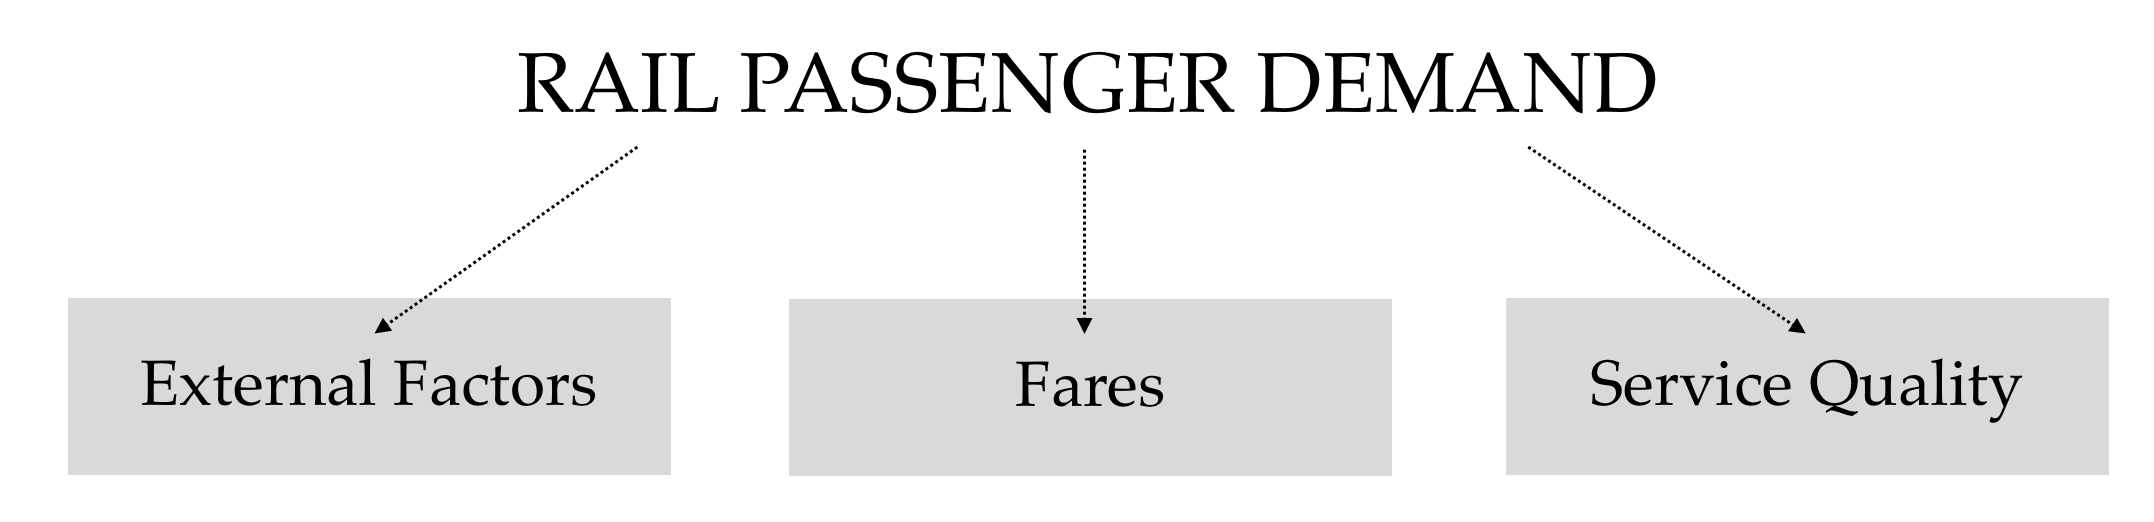
\includegraphics[scale=0.3]{drivers-demand}
\caption{Drivers of rail passenger demand.}
\label{fig:drivers_demand}
\caption*{Source: \cite{pdfh}, Chaper B0, page 1 [adapted]}
\end{figure} 

The first group, as the name says, comprises aspects that are not under control of the train companies. In broad terms, they are related to economic, socio and demographic aspects of the region. Additionally, the availability, quality and cost of competitive modes - car, bus, coaches and air services, are considered.

The second group regards the fares. Despite the evident impact of fares in the demand, the PDFC has been struggling in quantify this impact when it regards how different type of tickets affect their demand, which is the central issue of this work. It will be convenient to extend the discussion about the different types of fares to better interpret the issues around the estimation of the relationship between demand and fares. It will be done in the next section.

% As will be discussed in the sections ahead, several approaches have been tried to quantify these impacts, however, they failed in report coherent and consistent measures. The purpose of this study to apply Bayesian methods to estimate fare elasticity of demand an alternative method to quantify those effects is related to this difficulty

The third group involves the service quality and includes the biggest range of sub elements. The PDFH subsets it as four aspects: 

\begin{enumerate} [label=(\roman*)]
\item Timetable and related features, which covers journey time, frequency and interchange and is usually summarized in the \textit{generalised journey time} measure. 

\item Non-timetable attributes, which in turn comprises overcrowding, rolling stock quality, onboard facilities, station facilities, provision of passenger information, staff and security, cleanliness, advertising and promotion. 

\item Reliability, which covers punctuality and cancellation. 

\item New services and access, which regards the potential demand hold by new services in new or existing routes, new station and also the effects of improving accessibility to stations.
\end{enumerate}

It is noticeable, thus, that the rail passenger demand is considered to be implicated by several factors. For the fare elasticity estimation, however, the demand model is usually simplified to hold fewer elements that are deemed to represent the mass of the covariance of the others drivers of demand. 

Equation \ref{eq:demand_pdfh} presents the short version of demand model.

\begin{equation}
\label{eq:demand_pdfh}
V_{i} = a \; \text{GVA}^g_i \; P^f_i \; \text{GJT}^\gamma_i
\end{equation}
where

$V_i$ is volume of journeys;

$a$ is a constant;

$GVA_i$ is the gross added value;

$P_i$ is the price of the ticket;

$GJT_i$ is the generalised journey time;

$g$ is the GVA elasticity of demand;

$f$ is the price elasticity of demand;

$\gamma$ is the GJT elasticity of demand.
\\[3pt]

This simplification is relevant because for the estimation of individual fare elasticities it is necessary to expand the component price for as many fares as exist, which can make the model inherently complicated. Thus, to keep it simple without losing much information, previous studies have established this simple version \citep{its-systra-report}, which will also be adopted in this study. 

Additionally, as one may notice, the replacement of GDP by GVA is due to the effort to regionalize the income effect across routes \citep{pdfhv5}. Therefore, instead of applying a national GDP, GVA  data is more suitable, since it is available in the NUTS \footnote{Nomenclature of territorial units for statistics.} 3 level.

\section{Rail fares in the UK}

\subsection{Rail fares taxonomy}

\textit{Standard, first class, saver, super saver, single, return, season, peak, off-peak, advance}. Despite one may judge the taxonomy of rail fares to be self-explanatory at a first glance, it can be confusing to structure them into a cohesive system because of the diversity of names and classification used in different types of documents. 

% Appealing to official documents may not help in which regards taxonomy since they usually refer to fares as their terms and conditions, instead of having a classification. This lack of structure is understandable since the regulated fares cover only part of the possible existent fares. Therefore acts, franchising agreements and other official documents do not necessarily mention fares that are defined on a commercial basis; established subject to the strategy of the train operating company.

% It seems, therefore, that the rail taxonomy is a convention usual only to technical reports, even though it is not homogeneous. %For example, Table \ref{tbl:pdfh-fares}, shows the classification adopted in the PDFH. 

% 
\begin{table}[!ht] \centering 
  \caption{Fares Categories in PDFH} 
  \label{tbl:pdfh-fares} 
{\renewcommand\arraystretch{1.25}}
\begin{tabular} {llc}
\toprule
Category         & \multicolumn{2}{p{9cm}}{\raggedright Definition}\\
\hline
First            & \multicolumn{2}{p{9cm}}{\raggedright first class single and return and other first class services.}\\
Standard Open    & \multicolumn{2}{p{9cm}}{\raggedright full fare standard tickets, including standard day, single and return. } \\
Standard Reduced & \multicolumn{2}{p{9cm}}{\raggedright walk-up standard tickets, including saver, super-saver, cheap day return and network away breaks}\\
Standard Apex    & \multicolumn{2}{p{9cm}}{\raggedright includes standard advance purchase tickets. }\\
Seasons          & - \\ 
\bottomrule
\end{tabular}%
\caption*{Source: \cite{pdfh} , Chapter B2, Fares Elasticities, p. 2 [adapted]}
\end{table} 


After gathering different nomenclatures and definitions, they were compiled in Table \ref{tbl:fares-general} as a proposed taxonomy to be adopted in this study to interpret the RUDD's dataset classification. Because season fares will not be part of the scope of this is study they were not considered.


\begin{table}
 \centering 
  \caption{Fares categories and conditions} 
  \label{tbl:fares-general} 
{\renewcommand\arraystretch{1.25}}
\begin{tabular} {ccccccc}
\toprule
Type & \multicolumn{2}{c}{Coverage} & \multicolumn{2}{c}{Conditions}\\ 
\hline
\multirow{2}{*}{\textit{Full}}    & \multicolumn{2}{p{6cm}}{\raggedright \textit{full} or \textit{anytime} or \textit{open}, includes single and return, day single and day return.} & \multicolumn{2}{p{6cm}}{\raggedright Passengers can take any train.}\\
\hline
\multirow{2}{*}{\textit{Reduced}} &  \multicolumn{2}{p{6cm}}{\raggedright \textit{reduced} or \textit{off-peak} or \textit{saver/super saver}, includes single and return, day single and day return for off-peak and supper off-peak.} & \multicolumn{2}{p{6cm}}{\raggedright Passengers can take any off-peak train. Peak time may vary from route to route.}\\
\hline
\multirow{2}{*}{\textit{Advance}} & \multicolumn{2}{p{6cm}}{\raggedright \textit{advance} or \textit{apex}, sold only as single tickets.} & \multicolumn{2}{p{6cm}}{\raggedright Passengers can only take the specific train of the ticket. Must be bought in advance and has limited availability}\\
\bottomrule
\end{tabular}%
\caption*{Source: Own work}
\end{table} 



The three types of fares \textit{Full}, \textit{Reduced} and \textit{Advance} exist in both \textit{First} and \textit{Standard Class}. It will be common to abbreviated these names to their respective initial - $F$, $R$ and $A$, and represent the class as $1$ for \textit{First} and $2$ for \textit{Standard Class}. Thus, concatenating numbers and letters it is possible to make short reference to the fares - $1F$, $1R$, $1A$, $2F$, $2R$, $2A$. An exception for this taxonomy will be the abbreviation $1N$ (\textit{First Class Non-season}) used to refer to the three first class fares together (\textit{Full, Reduced} and \textit{Advance}).

The relevance given to taxonomy is due to the importance of correctly understanding the differences and particularities of tickets to properly interpret the market segmentation and the consumer behaviour. In the same sense, the next section approaches regulatory affairs since they may be useful to contextualise the results.


% the official documents - acts, francising agreements and other regulation documents - do not mention them as structured system of types and classes, but instead they are mentioned as conditions, or characterization, of the service. This may happen due to the fact that the regulated fares covers only part of the possible existent fares. Apart from the regulated fares, the frachisees have the freedom to set other fares in a commercial basis, limited to the conditions of the \textit{Ticketing \& Settlement Agreement} \citep{tsa} - a open boundary to the fare universe. 

% Notwithstanding the possibility of creation of new fares by the franchisees, one can consider the existence of a pattern in their general characteristics since there might be a common need of services with disregard to the franchise. For example, for whichever route that have potential for business clients, the franchise may have interest to have a first class fare. 

% In technical reports is possible to notice classifications which, despite not always structured, bring the ideia of standardization of terms and conditions of fares - \textit{standard, first class, saver, super saver, single, return, season, peak, off-peak} and \textit{advance}.
% % check whether the fares, when created, already receive those kind of names.

% For study purpose, however, the classification from the technical reports may be to wide and some clustering are necessary to allow more simple classification structure. For instance, the reccomendations of fares in the PDFH are based in a segmentation of tickets in five main categories, as shown in Table \ref{tbl:pdfh-fares}.


% By the end of this section, it will be presented an effort to match some names and characteristics of technical reports with te clustered structured of the PDFH. The latter one will be adopted in this study given the available classification of data and also for continuity purpose. 

% Before it however, the next subsection clarifies more aspects of rail fares.

\subsection{Regulated and non-regulated fares}

The rail fares in the Great Britain can be regulated, in which case they are set by the franchising authority, or unregulated, in which case they are set by the train operating companies on a commercial basis \citep{fares-ticketing}. 

According to the last review, run by the Strategic Rail Authority in 2003, there are two groups of regulated fares: the \textit{protected fares} and the \textit{commuter fares} \citep{fares-ticketing}. The regulated fares are set in a price-cap mechanism, where the X may vary according to the objectives of the regulatory policy. Since 2004 it became RPI+1\% \citep{fares-ticketing}.

The \textit{protected fares} seems to serve the broad guidances of regulation policy as they assure reasonable and affordable fares \citep{fares-ticketing}, whilst allows train companies to commercially exploit the route through market segmentation and unregulated fares. According to the taxonomy adopted in the SRA's report \citep{sra-conclusions}, this group of fares comprises:

\begin{itemize}  
\item \textit{Saver returns}, which regards off-peak services, available for most long-distance journeys. In the taxonomy shown on Table \ref{tbl:fares-general} it would be classified as \textit{Reduced}.
\item \textit{Standard returns}, which regards the full-fare and allows the passenger to travel anytime, but only for journeys without the \textit{saver} option. In that taxonomy shown on Table \ref{tbl:fares-general} it would be classified as \textit{Full}.
\item \textit{Weekly season}, others than the ones included in the \textit{commuters fares}. In the taxonomy shown on Table \ref{tbl:fares-general} they would not appear since they regard season fares and others not covered in this study.
\end{itemize}

It is interesting to notice that the regulated fares cover at least one type of ticket that must be available, so a passenger without time restrictions can access the basic service at affordable prices. There is left commercial spots to be price discriminated, targeting users with more strict preferences.

The regulation of \textit{commuter fares} affects mostly season tickets, as well other types as standard single and return within the London Travelcard area or from a pre-defined area of London's suburbs \citep{sra-conclusions}. Because the London area and commuters tickets are out of the scope of this work, they were mentioned just for completeness, but no light will be shed on them.

\section{Fare elasticities of demand}

\subsection{Definition}
The fare elasticities of demand represent the relationship between the demand for a type of fare and the prices of the fares available in the market -  how much the quantity demanded changes when these prices change. It is calculated as the percentage change in quantity demanded by the percentage change in prices, as shown in Equation \ref{eq:elasticity}.

\begin{equation}
\label{eq:elasticity}
\eta = \frac{\% \Delta Q }{\% \Delta P}
\end{equation}
where
% \begin{flalign*}
% \begin{split}
% &\eta \; \text{is the price elasticity of demand} \\
% &Q \; \text{is the quantity demanded} \\
% &P \; \text{is the price}\\
% \end{split}
% \end{flalign*}

$\eta \; \text{is the price elasticity of demand}$

$Q \; \text{is the quantity demanded}$

$P \; \text{is the price}$
\\[3pt]

The fare elasticities of demand may regard the change in the demand of a good $A$ given a change in the price of the good itself, which is called the own-elasticity, shown in Equation \ref{eq:own-elasticity}; or it may regard the change in the demand of a good $A$ given a change in the price of good $B$, which is called cross elasticity, shown in Equation \ref{eq:cross-elasticity}. 

\begin{equation}
\label{eq:own-elasticity}
\eta_{AA} = \frac{\% \Delta Q_A }{\% \Delta P_A}
\end{equation}
where 
% \begin{align*}
% \begin{split}
% &\eta \; \text{is the price elasticity of demand of good $A$ with respect of changes in the price of good $A$} \\
% &Q \; \text{is the quantity demanded of good $A$} \\
% &P \; \text{is the price of good $A$} \\
% \end{split}
% \end{align*}

$\eta$ is the price elasticity of demand of good $A$ with respect to changes in the price of good $A$;

$Q$ is the quantity demanded of good $A$;

$P$ is the price of good $A$.
\\[3pt]


\begin{equation}
\label{eq:cross-elasticity}
\eta_{AB} = \frac{\% \Delta Q_A }{\% \Delta P_B}
\end{equation}
where 
% \begin{align*}
% \begin{split}
% &\eta \; \text{is the price elasticity of demand of good $A$ with respect of changes in the price of good $B$} \\
% &Q \; \text{is the quantity demanded of good $A$} \\
% &P \; \text{is the price of good $B$} \\
% \end{split}
% \end{align*}

$\eta$ is the price elasticity of demand of good $A$ with respect to changes in the price of good $B$;

$Q$ is the quantity demanded of good $A$;

$P$ is the price of good $B$.
\\[3pt]

According to economic theory, the own-elasticity of normal goods, say good A, is expected to be negative indicating that the more the price of good A rises, the lower its demand will be. Conversely, the cross-elasticity of a substitute of a normal good A, say good B, is expected to be positive indicating that the more the price of good B rises, the higher the demand of the good A will be because consumers tend to trade-off to the cheaper good.

The degree of competition between two goods depends upon how close substitutes they are. If two goods are close substitutes, switching from one to another is likely to happen so they become very price sensitive. In other words, if two goods are close substitutes they should have high cross price elasticities.

According to the PDFH, there is a belief that the range of fares covered in this study ($1F$, $1R$, $1A$, $2F$, $2R$ and $2A$) are substitute goods, since they assume that for these fares ``the own elasticity will be negative and the cross elasticities positive" \citep[p.~8, Chapter B2]{pdfh}. 

In fact, they could be regarded as substitutes because ultimately they provide a transport service from one place to another. However, they might differ in the degree of competition, since particularities and specific conditions of each fare are supposed to segregate these markets. 

The extent of this segregation is valuable knowledge. Investigating the fare elasticities of different types of tickets may allow identifying how close these markets really are. 

Additionally, it may reveal different dynamics with regard to the others drivers of demand. For instance, customers of a given type of fare may be more sensitive to service quality than others.

% \begin{align}
% \label{eq:d1f}
% & D_{F} = k{F} \; {P_{F}}^{\eta_{FF}} \; {P_{R}}^{\eta_{FR}} \; {P_{A}}^{\eta_{FA}} \; {P_{f}}^{\eta_{Ff}} \; {P_{r}}^{\eta_{Fr}} \; {P_{a}}^{\eta_{Fa}}\\
% & D_{R} = k{R} \; {P_{F}}^{\eta_{RF}} \; {P_{R}}^{\eta_{RR}} \; {P_{A}}^{\eta_{RA}} \; {P_{f}}^{\eta_{Rf}} \; {P_{r}}^{\eta_{Rr}} \; {P_{a}}^{\eta_{Ra}}\\
% & D_{A} = k{A} \; {P_{F}}^{\eta_{AF}} \; {P_{R}}^{\eta_{AR}} \; {P_{A}}^{\eta_{AA}} \; {P_{f}}^{\eta_{Af}} \; {P_{r}}^{\eta_{Ar}} \; {P_{a}}^{\eta_{Aa}}\\
% & D_{f} = k{f} \; {P_{F}}^{\eta_{fF}} \; {P_{R}}^{\eta_{fR}} \; {P_{A}}^{\eta_{fA}} \; {P_{f}}^{\eta_{ff}} \; {P_{r}}^{\eta_{fr}} \; {P_{a}}^{\eta_{fa}}\\
% & D_{r} = k{r} \; {P_{F}}^{\eta_{rF}} \; {P_{R}}^{\eta_{rR}} \; {P_{A}}^{\eta_{rA}} \; {P_{f}}^{\eta_{rf}} \; {P_{r}}^{\eta_{rr}} \; {P_{a}}^{\eta_{ra}}\\
% \label{eq:d2a}
% & D_{a} = k{a} \; {P_{F}}^{\eta_{aF}} \; {P_{R}}^{\eta_{aR}} \; {P_{A}}^{\eta_{aA}} \; {P_{f}}^{\eta_{af}} \; {P_{r}}^{\eta_{ar}} \; {P_{a}}^{\eta_{aa}}
% \end{align}
% where 
% \begin{align*}
% \begin{split}
% & D_{j} \; \text{are the demand of fare $j$} \\
% & P_{j} \; \text{are the price of fare $j$} \\
% & \eta_{jj} \; \text{are the price elasticity of demand - own and cross, as shown in Equations \ref{eq:own-elasticity} and \ref{eq:cross-elasticity}} \\
% &k_{j} \; \text{are constants.}
% \end{split}
% \end{align*}


\subsection{Difficulties and issues}

As introduced in Chapter \ref{chp:introduction}, estimating fare elasticities is not straightforward.  Indeed, it is being considered the most important area of disagreement on rail demand forecasting" \citep[p.~6]{its-systra-met}. This is so because the traditional estimation of elasticities with the aid of ordinary least squares (OLS) models is hindered by the high correlation of the fares. 

Even though it does not cause bias, the high correlation is a known problem in OLS estimation. When the independent variables are highly correlated it is difficult to isolate individual effects of each variable since most of the variation will be common to both. It leaves the OLS with little information to estimate and because of it, the output might be poor estimates. 

Another way to interpret the high correlation problem regards the fact that when regressors are highly correlated, it is difficult to identify and address the explanatory power among the variables. This fluctuation causes high variances in the estimators causing them not to be precise. It is like their effects in the dependent variable are blurred together and there is low certainty about which one holds which part of it.

In Bayesian inference, however, correlation gains a new perspective. When two predictors are correlated, their coefficients tend to be anti-correlated, which means the bigger one is, the smaller the other will be. In other terms, one can say that ``correlation of predictors causes estimates of their regression coefficients to trade-off" \citep[p.~513]{kruschke2014}. 

That feature can be very useful depending on how the prior distributions are defined in the Bayesian model. When non-informative priors are adopted the blurred effect - the large variance, usual to the OLS  estimation - is reflected in both posterior density of the estimated coefficients. This means that both coefficients will be estimated with a large range of credible values. However, when a strong prior distribution is defined for one coefficient, which means that one is applying a strong belief to constraint its value, it simultaneously constraints the value of the correlated variable, because of their anti-correlation. 

Therefore, when variables are strongly correlated, the constraint applied to one coefficient may ``propagate to the estimates of regression coefficients on other predictors that are correlated with the first" \citep[p.~525]{kruschke2014} and correlation may not be a problem anymore.

There is also the risk of the predictor variables being correlated with omitted variables. In this case, for both methods, it may mislead the interpretation of the coefficients. It worths recovering that an omitted variable, when correlated with a predictor, impacts the predictor estimation to the extent of their correlation \citep{studenmund2011}. Because the remedies to avoid omitted variable bias are related to the theoretical consistency of the model, which was adopted from previous studies, it will not be covered here. 

\subsection{Previous studies}

Several attempts have been tried to solve the issue of estimating fare elasticities applying ticket differentiation. \cite{wardman2003} were the first to estimate consistent own and cross-elasticities, with the correct sign and statistically significant. The successful model applied two theoretical constraints known as ``Slutsky Symmetry" \citep{wardman2003} and ``Dodgson Relationship" \citep{wardman2003}. However, the weakness of this study was the absence of \textit{Advance} ticket, ``although they were very much in their infancy" \citep{its-systra-report}.

A later study of \cite{its-systra-report} have recovered this method to update the evidence and introduce the \textit{Advance} fare in the estimation. However the conclusion was that ``econometric by itself was not able to estimate definitive fare elasticities, but market research would be required in addition" \citep[p.~93]{its-systra-report}.

The mix of revealed preference data with stated preference data turns out to be the more consistent approach. Nevertheless, the authors have concluded that this method has presented a weak performance in some markets segments - especially short distance, which brought vulnerability to it.

As one may notice what all these methods have in common is that they were based on the sampling theory approach. However, ``unrestricted least-squares estimates of own- and cross-price elasticities are often of incorrect sign and unreasonable magnitude" \citep[p.~413]{montgomery1999} and even the usage of contrivances have not achieved satisfactory estimates that can be generalised.  Because of the struggle of the methods attempted so far, it was considered reasonable the exercise to estimate the fare elasticities with the aid of Bayesian regressions.

\section{The bayesian approach}

The Bayesian promise for elasticity estimation is primarily a solution ``to get rid of the wrong signs" \citep[p.~36]{griffiths1988}. The advantage of the Bayesian econometrics is the simple way to incorporate prior information from economic theory \citep{griffiths1988}, which helps to achieve reasonable estimates. 

Beyond that, hierarchical Bayes model has been reported as successful solutions for more complex elasticities estimation \citep{liu2009}. They are useful to problems when it is possible to identify ``meaningful hierarchical structure" \citep[p.~221]{kruschke2014}, in which the parameters can be estimated with the aid of layers of information funnelling from general to specific. For instance, \cite{montgomery1999} have estimated price elasticities of multiple brands and stores with the aid hierarchical model. In this work, the authors are aware of the problem of customizing elasticities estimation from a national level to a regional market, or even store to store, which is the description itself of the hierarchical nature of the problem. The results were reported by the authors as ``reasonable cross-price elasticities estimates while retaining much of the interesting and potentially valuable store-to-store variation" \citep[p.~414]{montgomery1999}. 

As seen, the applications of Bayesian econometrics to elasticity estimation are full of potential. However, because this is an introductory work on the subject,  hierarchical models will be out of scope, and the focus will be strict to the simplest application o Bayesian regression. The next section work on basic concepts of it. 

\subsection{Bayes' theorem}

The Bayesian approach is based on updating the credibility of a prior belief in the light of relevant information, which is the data observed. This abstract rationale becomes a statistical tool through the Bayes' theorem, which is presented in Equation \ref{eq:bayes}.

% \begin{equation}
% \label{eq:bayes}
% 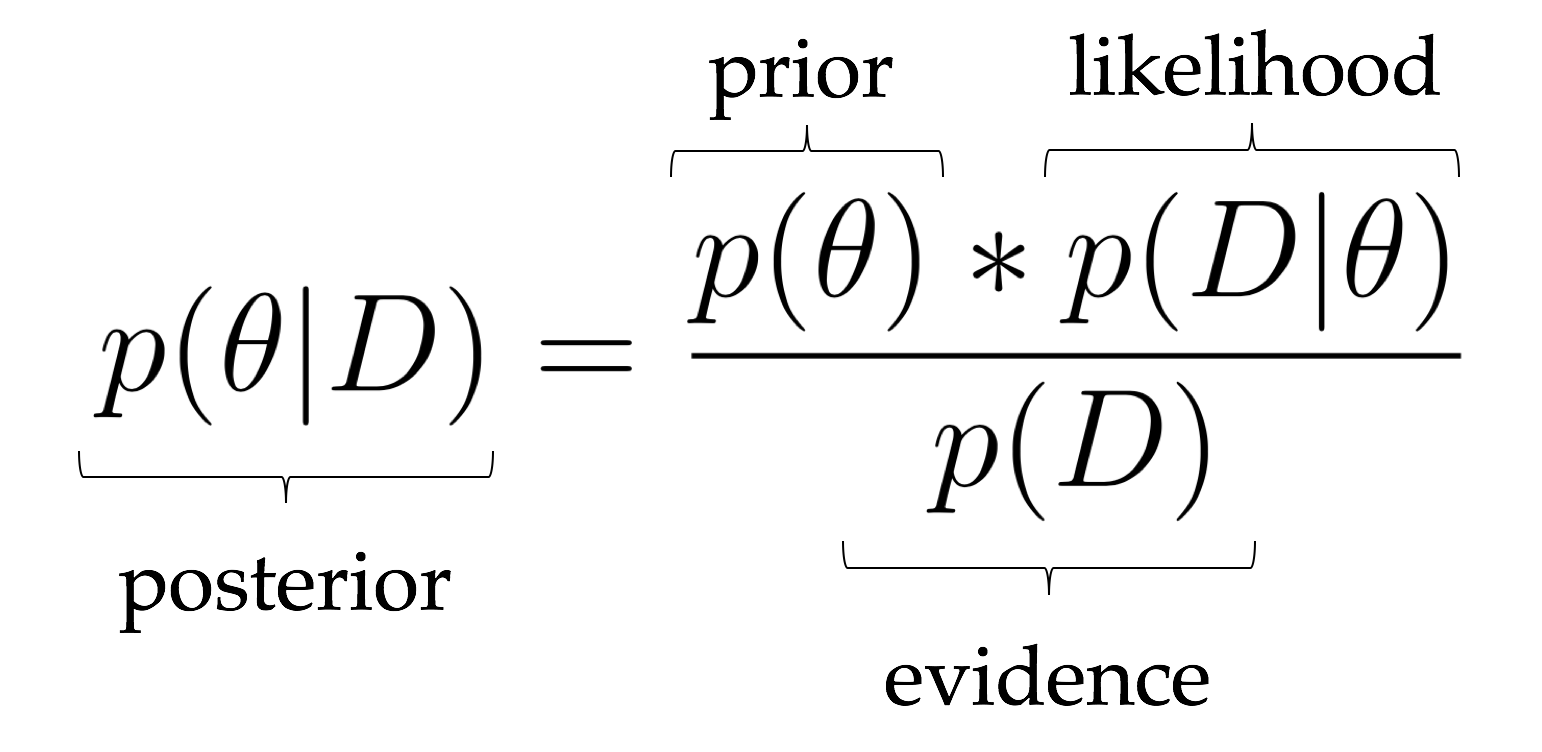
\includegraphics[scale=0.2]{bayes-theorem}
% \end{equation}

\begin{align}
\label{eq:bayes}
  \underbrace{p(\theta \mid D)}_\text{posterior} =  \frac{\overbrace{p(\theta)}^\text{prior} \cdot \overbrace{p(D \mid \theta)}^\text{likelihood}}{\underbrace{p(D)}_\text{evidence}}
\end{align}


where 
\begin{align*}
\begin{split}
&\theta \; \text{is the parameter under study; and} \\
&D \; \text{is tha data observed. It can be thought as a random variable $Y$} \\
& \quad \text{with observations $y_i$}
\end{split}
\end{align*}

The $p(\theta|\text{Data})$ is called the posterior probability density function and represents the updated belief regarding the parameter $\theta$, given an observed data. It is the answer to questions like ``Given the data, what do we know about $\theta$?" \citep{koop2003}.

The $p(\theta)$ is called the prior probability density function. It represents the pre-existent belief regarding $\theta$, unconditional to the observations. The prior belief may be defined due to a theoretical background or to any kind of accumulated knowledge of the subject. 

That is often a critique of the Bayesian approach, being considered a subjective element in the analysis which may pollute the final results. However, a good effect of it is that it demands the researcher to have a prior interpretation of the phenomenon under study and consider reasonable values that it may assume. Indeed, the practice of interpreting a problem before looking at the estimated parameters of a model is highly recommended in the frequentist inference (\cite{gujarati2009}, \cite{kennedy2003}, \cite{studenmund2011}). 

Also, it is important to highlight that the establishment of a prior probability density might not be a mere researcher's opinion. On the contrary, it must be justified to a ``sceptical and scientific audience" \citep{kruschke2012}. Even whether sceptics disagree about the distribution of a prior, there is still the advantage of measure the impact of the disagreement testing the impact of different priors on the final estimate.

The $p(D|\theta)$ represents the likelihood function, which is a function of the parameter $\theta$ for a given data $Y$ assuming that $\theta$ follows a given probability distribution. \cite{gujarati2009} teaches that one may think the likelihood and the probability density function as related functions that are both composed of three parts: i) the parameter under study, $\theta$; the data $Y$, whose observations are $y_i$; and the probability distribution of the parameter under study - how it is expected to behave. It may be useful thinking the function as the analogy of a machine with inputs and outputs. When the input is a possible value of the parameter under study $\theta$, it is the likelihood function, which uses the other two pieces of information to generate the output - the likelihood. Whether the input is the observed data, $y_i$, it is a probability function, which uses the other two pieces of information to generate the output - the (joint) probability of observing $y_i$. 

 % the likelihood ``specifies the probability of values of the predicted variable as a function of the values of the predictor values \citep[p.~421]{kruschke}.

The last element in the Bayes' theorem is the $p(D)$, which represents the observed data. It may be interpreted as the unconditional probability of observing a given $Y$, in the whole universe of possibilities. However, because the interest regards in learning about the parameter under study $\theta$, and $p(D)$ is not related to it, it is usually not considered in the analysis. 

Because of that, it is usually said that the posterior probability density is \textit{proportional} to the prior probability density and the likelihood, as shown in Equation \ref{eq:proportional-bayes} \citep{koop2003}. 

\begin{equation}
\label{eq:proportional-bayes}
p(\theta \vert D) \propto p(\theta) * p(D \vert \theta)
\end{equation}

% An interesting insight about the Bayes's theorem regards the fact that it is based in simple rules of probability. Consider, for instance, two random variables $A$ and $B$, illustrated in Figure \ref{fig:venn-diagram}. 

% \begin{figure}[H]
% \centering
% 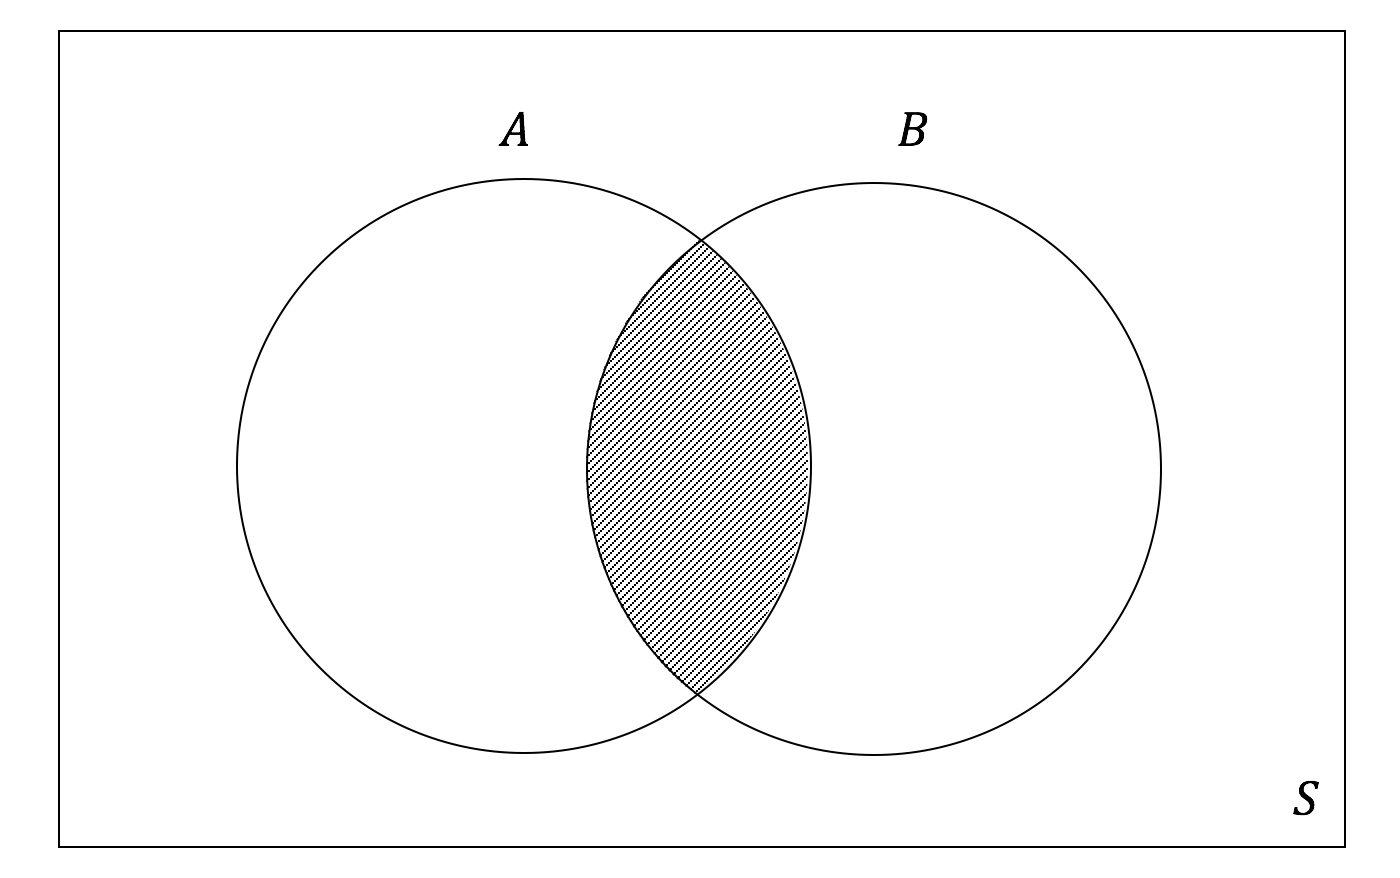
\includegraphics[scale=0.3]{venn-diagram}
% \caption{Venn diagram of sample space $S$ with events $A$ and $B$.}
% \label{fig:venn-diagram}
% \caption*{Source: \cite{montgomery2010} p.24}
% \end{figure} 

% If one is interested in the probability of an event in the shaded area, which means the probability of $A$ and $B$ happening ($ A \cap B$), the rule of the joint probability would state:

% \begin{align}
% \label{eq:joint-prob}
% p(A, B) &= p(B \vert A)*p(B) \quad \text{, or equivalently} \\
% p(A, B) &= p(A \vert B)*p(A)
% \end{align}

% Equaling these two equations, one could achieve a generic format of the Bayes' theorem, as shown in Equation \ref{eq:joint-prob2}, where $A$ would represent $\theta$ and $B$ would represent $D$. 

% \begin{align}
% \label{eq:joint-prob2}
% p(A \vert B) = \frac{p(B \vert A)*p(B)}{p(A)} 
% \end{align}

% At this point, it should be highlighted that the parameter under study in a bayesian inference is random variable. This is the fundamental diference between the bayesian and the frequentist assumptions. Whilst the frequentist approach is chasing the \textit{true} parameter, for instance, the true $\beta$ in a regression, the bayesian assumes that the parameter is a variable itself, and, as such, one should not refer to its \textit{true} value, but to its probability distribution since it can assume a given range of values with different probabilities associated to eachof these values.

\subsection{Running a bayesian regression model}

\textit{Model definition}

Expanding the Bayesian theorem to a practical application in a regression model does not change the Bayes' rationale. However, it may be useful making some explicit considerations since, instead of a unidimensional problem - as presented before, this study will regard a multi dimensional problem because the interest is to estimate several parameters together.

To easily illustrate, consider a regression model with two parameters of interest $\beta_{0}$ and $\beta_{1}$, as given by Equation \ref{eq:regression-model}. 

 \begin{equation}
\label{eq:regression-model}
\hat{y}_{i} = \beta_{0} + \beta_{1}x_{1i}
\end{equation}

Assuming that $\beta_0$ and $\beta_1$ are normally distributed with mean $M_0$ and $M_1$ and standard deviation $S_0$ and $S_1$, respectively, as shown by Figure \ref{fig:prior-likelihood-scheme}, then
\begin{figure}[H]
\centering
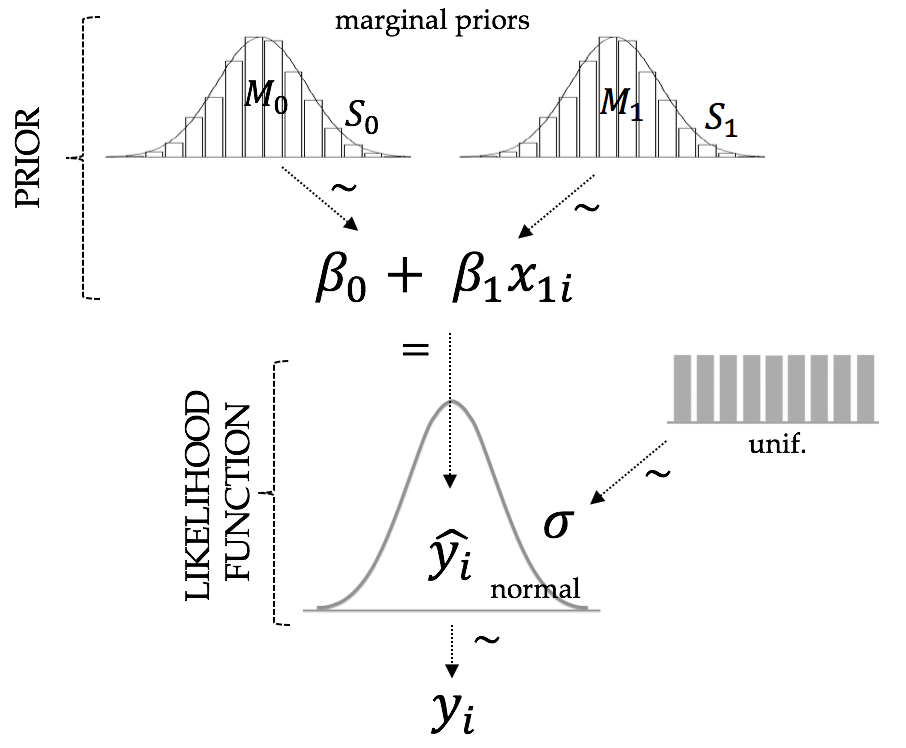
\includegraphics[scale=0.4]{prior-likelihood-scheme}
\caption{Bayesian regression scheme.}
\label{fig:prior-likelihood-scheme}
\caption*{Source: \cite{kruschke2012} p.727 [adapted]}
\end{figure}

\noindent the characterization of the prior probability density would be a three-dimensional space, as shown by Figure \ref{fig:prior-space-prob}. One may notice that the prior is a joint probability of $\beta_0$'s and $\beta_1$'s individual - or marginal - prior probability densities, which integrates to 1.

\begin{figure}[H]
\centering
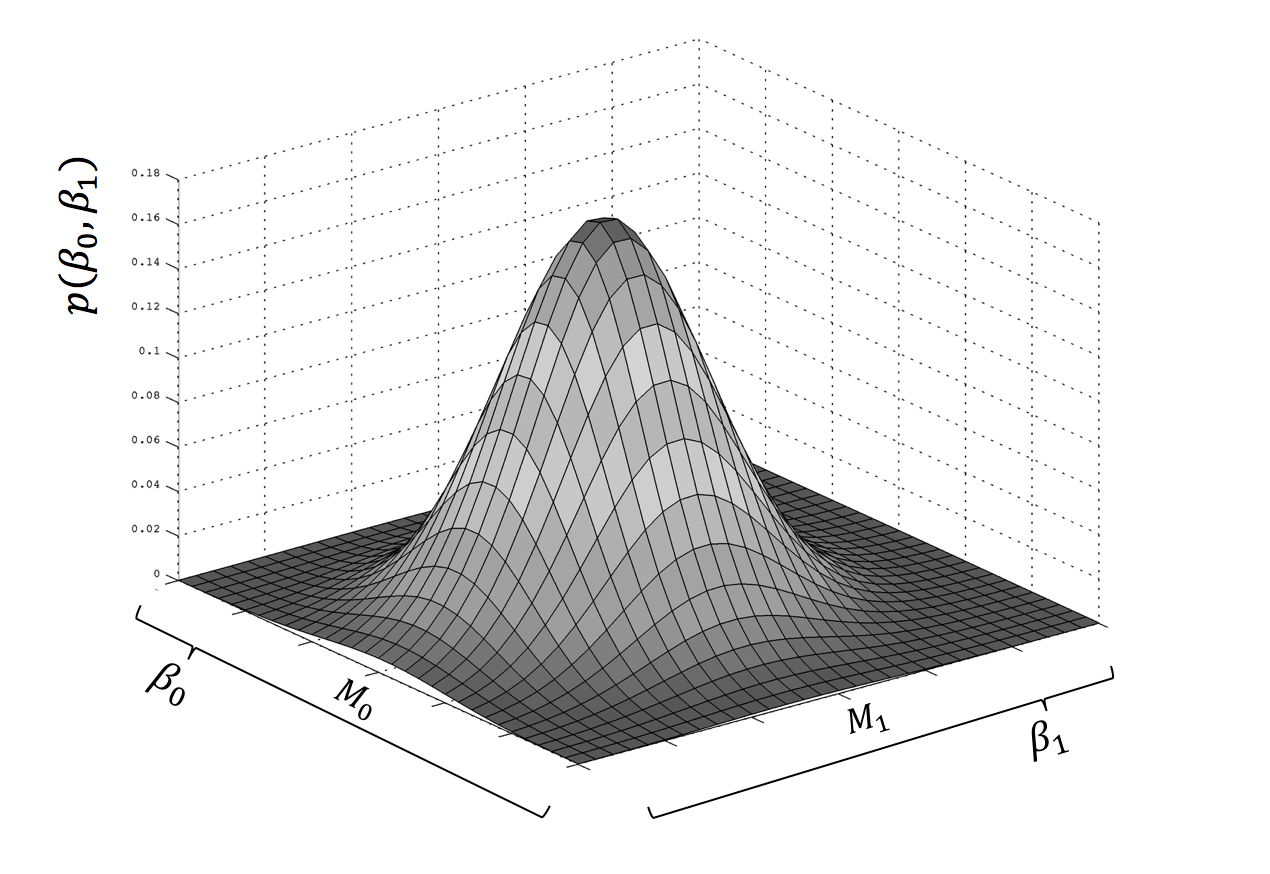
\includegraphics[scale=0.5]{prior-space-prob}
\caption{Prior probability density for parameters $\beta_0$ and $\beta_1$.}
\label{fig:prior-space-prob}
\caption*{Source: Own work}
\end{figure}

The second element to define a Bayesian regression model is the likelihood function, also illustrated in Figure \ref{fig:prior-likelihood-scheme}. In this example, it was assumed that the predicted variable $Y$, which has $y_i$ realizations, is normally distributed with mean $\hat{y}_i$ - which can also be interpreted as $\hat{y}_i = \beta_{0} + \beta_{1}x_{1i}$, and standard deviation $\sigma$. The arrow linking the $\beta$s with the $\hat{y}_i$ shows that there is an equality between it, so $y_i$ is a linear function of the explanatory variables.

A formal way to state this model could be as presented in Equation \ref{eq:model_example}.

\begin{align}
\label{eq:model_example}
\text{y}_i \sim& Normal(\hat{y}_i, \sigma) && \text{[likelihood]} \\
\hat{y}_i =& \beta_{0} + \beta_{1}x_{1i}     && \text{[linear model]}\nonumber\\
\beta_0 \sim& Normal (M_0, S_0) && \text{[prior]}\nonumber\\
\beta_1 \sim& Normal (M_1, S_0) && \text{[prior]}\nonumber\\
\sigma \sim& uniform(a,b) \nonumber          && \text{[prior]}
\end{align}
\\[3pt]

\textit{Estimation of the posterior}

Once defined these elements in the Bayesian regression framework, the result will be a posterior probability density. Analogously to the prior, the posterior will be multidimensional probability space which integrates to 1, similarly to Figure \ref{fig:prior-space-prob} - the exact shape of the posterior will depend on the prior and the likelihood. 

Still analogously to the prior probability density, the posterior is a joint probability space compounded by the marginal posterior distribution of each predictor, in this example $\beta_0$ and $\beta_1$.

The posterior probability density is generated by approximation by collecting from it a large representative sample. This method, called Markov Chain of Monte Carlo - MCMC, is useful when the analytical solution is not possible given the complexity of the posterior distribution \citep{kruschke2014}. ``It is the MCMC algorithms and software, along with faster computer hardware, that allows Bayesian data analysis for realistic applications that would have been effectively impossible 30 years ago"\citep[p.~144]{kruschke2014}.

The core idea of an MCMC lies in the generation of a sequence of samples in the probability space through a random walk process - it may vary among software and algorithms. Each sample is virtually equivalent to a step in the random walk, in which is defined a value for all predictors in the model. For instance, in the example used so far, a step would contain a pair of $\beta_0$ and $\beta_1$ ($\beta_0$, $\beta_1$). 

The random walk is the way the algorithm explores the probability space of possible values. To decide whether or not to accept a step, the algorithm compares the probability of the current step with the probability of the proposed step and applies a decision rule - which may also vary among software and algorithms. These probabilities used in to decide whether or not a proposed step should be accepted are computed from combinations of the prior and the likelihood - recover Equation \ref{eq:proportional-bayes}.

From a given position, the next step is accepted as credible value if the combined probability of the likelihood and the prior is bigger than the current step. If the next step has the lower probability, then a specific decision rule determines whether it is accepted or not. The practical effect is that the MCMC always accepts a step - and keep it as a sample - to explore regions where the probability space has high probability and only accepts part of the steps in regions with lower probability. With long MCMC, there would have been enough steps to provide a good approximation of the posterior probability density. 

\chapter{Methods}
\label{chp:methods}
%(4.000 words/2.500)

\section{Data}

The available dataset for the current study is a subset of the \textit{Rail Users and Drivers Dataset} - RUDD, for non-London long distance (over twenty miles) journeys. 

Th RUDD ``includes just over a twenty thousand flows, for twenty-one years (1994/95 to 2013/15), with each flow including more than 900 variables" \citep[p.~135]{systra_rand}. In the current application of RUUD, the data regards 6184 bi-directional origin-destination pairs with annual information volume of journeys and revenues, and some drivers of demand. Figure \ref{fig:stations} illustrates all stations comprised in these OD pairs.

% operational information as journey time, interchange penalty and frequency penalty that are summarised in the variable generalised journey time. Additionally it also brings external variables as , population, employement, inflation and some data of competitive modes (cars and bus). - Figure \ref{fig:stations} illustrates all stations comprised in these OD pairs.

\begin{figure}[H]
\centering
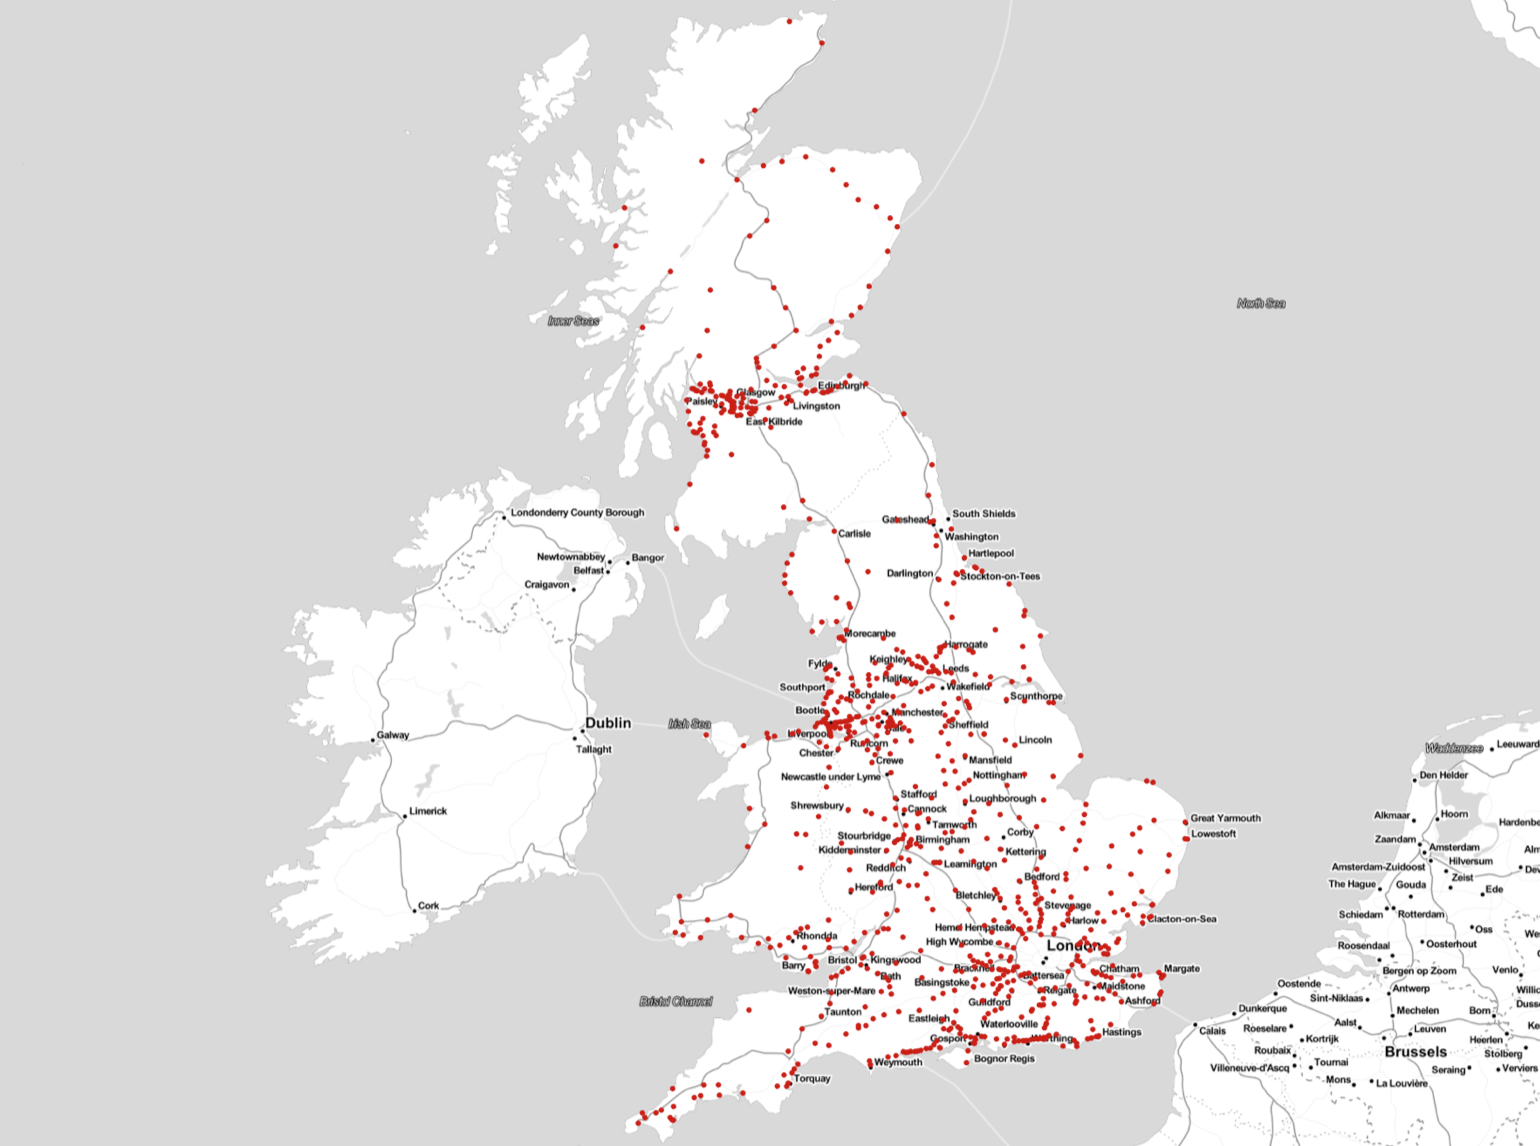
\includegraphics[width=\linewidth]{stations1}
\caption{Stations covered in the 6.184 OD pairs of the RUDD's subset}
\label{fig:stations}
\caption*{Source: Own work}
\end{figure} 

% The dataset also contains information about a set of drivers of demand, but, as discussed in Chapter \ref{chp:lit-rev}, the variables of interest for this study will be restricted to gross value added (GVA) and generalised journey time (GJT), in addition to the volume of journey and revenue variables.

\subsection{Variables}

As discussed in Chapter \ref{chp:lit-rev}, the variables of interest for the current work will be journeys, fares, generalised journey time, and gross added value. This section is dedicated to discuss these variables, what they mean and some particularities about what they actually represent. 

To start it should be highlighted that the variable fares are not directly collected. Instead, it will be approximated by the average revenue per journey. The fact that the main variable in the study is not actually known may represent a vulnerability, nevertheless, it would not be further debated since it is the best information at hand.

Another fact is that, because the dataset is bi-directional, it means that, for example, a trip from Leeds to York and from York to Leeds are identified by the same code, and the variables of journeys and revenues regard both directions summed up. Also, the GVA was collapsed into a single measure that reflects the average GVA of the origin and destination regions. It is, therefore, helpful to consider the OD pair as a connexion, or a route, since the variables will always regard the pair, instead of the location of the origin or the destination by itself. Table \ref{tbl:var_units} summarises information on the variables.


\begin{table}[!ht] \centering 
  \caption{Definition of variables} 
  \label{tbl:var_units} 
{\renewcommand\arraystretch{1.25}}
\begin{tabular} {lllll}
\toprule
Variable          & \multicolumn{2}{m{6cm}}{\raggedright Measure and Unit} & \multicolumn{2}{m{5cm}}{\raggedright Conexion Equivalent Measure} \\
\hline
\textit{Journey}  &\multicolumn{2}{m{6cm}}{\raggedright annual volume of tickets sold, by fare type.} 
				  &\multicolumn{2}{m{5cm}}{\raggedright sum of origin and destina- tion values.}\\
\textit{Fares}    &\multicolumn{2}{m{6cm}}{\raggedright total annual revenue divided by annual volume of tickets sold, by fare type, 2014 values.} 
				  &\multicolumn{2}{m{5cm}}{\raggedright sum of origin and destina- tion values.}\\
\textit{GJT}      &\multicolumn{2}{m{6cm}}{\raggedright sum of journey time, frequency penalty and interchange penalty, as defined in PDFH, in minutes.} 
				  &\multicolumn{2}{m{5cm}}{\raggedright - }\\
\textit{GVA}      &\multicolumn{2}{m{6cm}}{\raggedright regional GVA, at NUTS 3 level, in millions of pounds, 2014 values.} 
				  &\multicolumn{2}{m{5cm}}{\raggedright simple average of origin's and destination's GVA.}\\
\bottomrule
\end{tabular}%
\caption*{Source: Own work}
\end{table} 



\textit{Journeys}

The variable \textit{journeys} is the number of tickets sold per year in each bi-directional route. It does not precisely reflect the number of trips since some tickets allow the passengers to break the journey in a route and make stopovers. Nevertheless, it is a good measure to represent the rail demand. 

To understand the dynamics of this variable Figure \ref{fig:jny} brings two dimensions of journeys: its trend across time and a characterization of journeys by distance.

As shown in Figure \ref{fig:jny_growth_agg} the volume of journeys have consistently increased in the past years. But which kind of journeys are these? Figure \ref{fig:jny_hist} shows that, despite there are very distant routes, as Plymouth to Inverness or Plymouth to Aberdeen, the mass of routes covered by the study peaks around 50 miles and is decrescent as the distance increases. Anyhow, one can affirm that no matter is the class of their length, the aggregate volume of journeys is increasing over the years for all of them, especially for journeys between 100 and 200 miles, as shown by Figure \ref{fig:jny_growth}. 

\begin{figure}[H]
\centering
\begin{subfigure}{\textwidth}
  \centering
  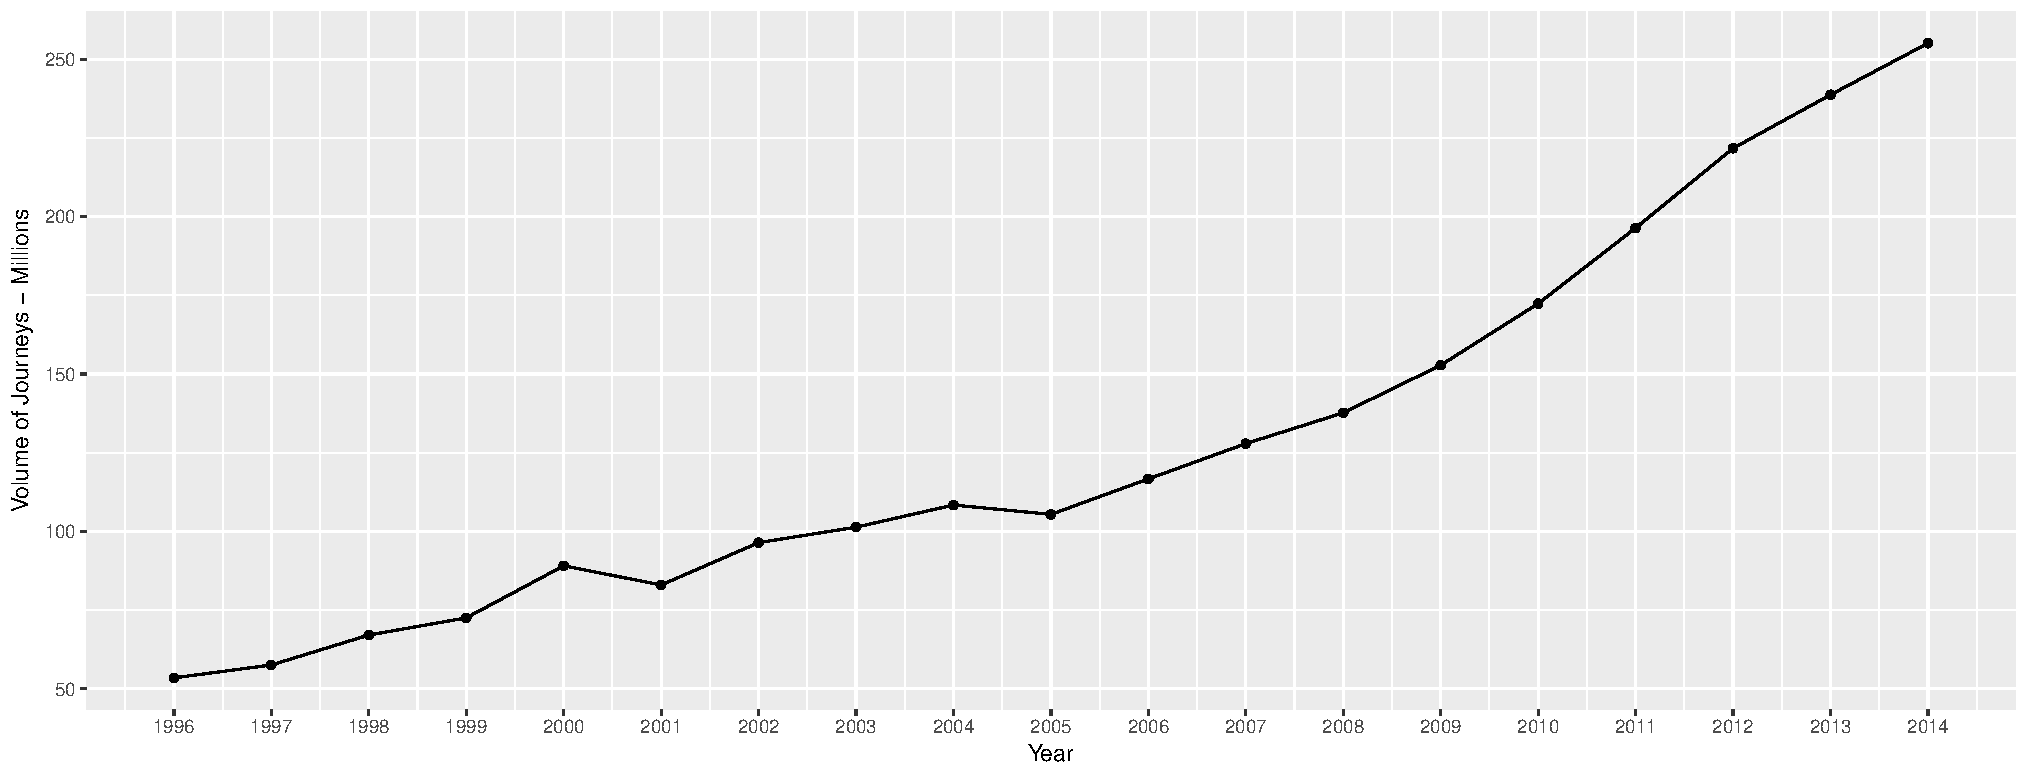
\includegraphics[width=\linewidth]{jny_growth_agg.pdf}
  \caption{Aggregated growth of journeys}
  \label{fig:jny_growth_agg}
\end{subfigure}%

\begin{subfigure}{.5\textwidth}
  \centering
  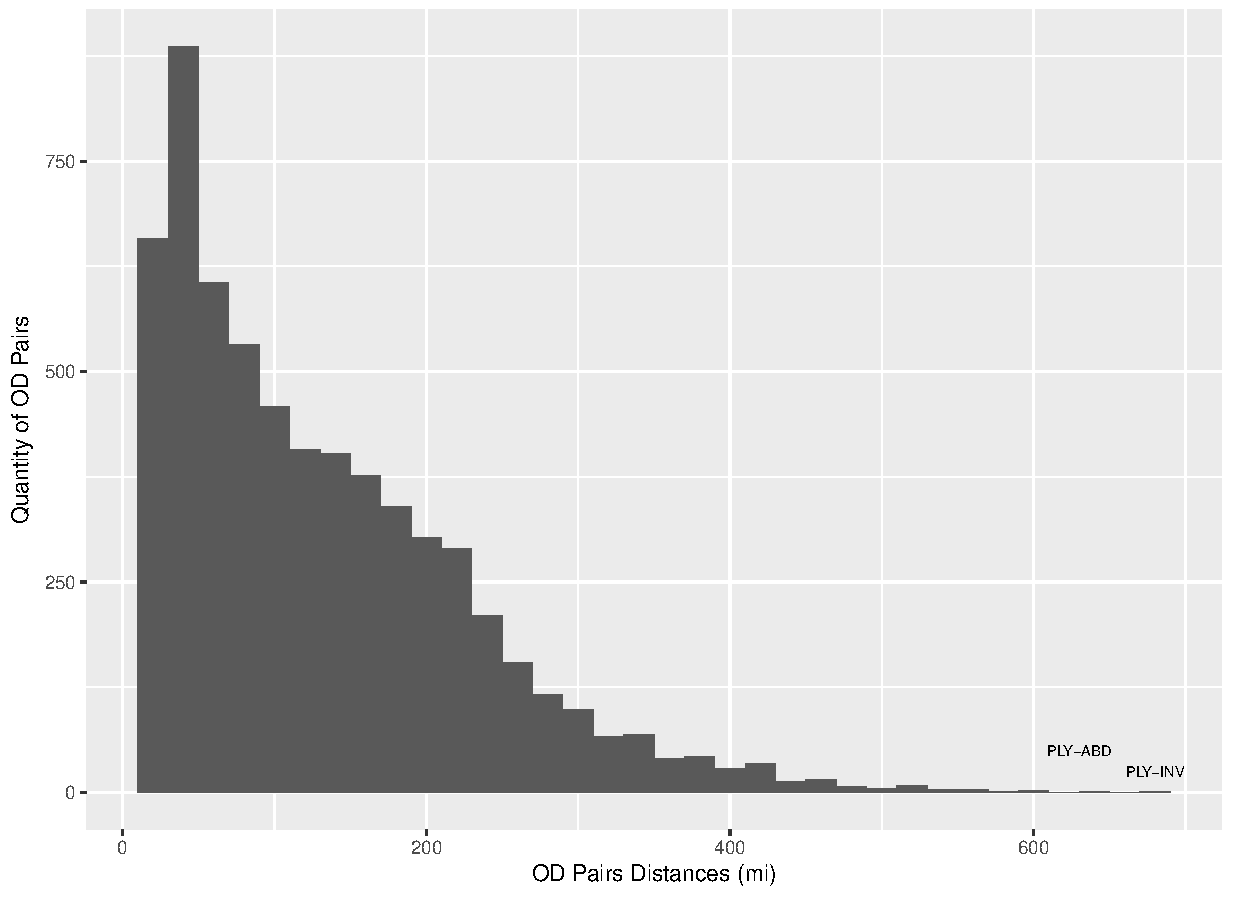
\includegraphics[width=\linewidth]{jny_hist}
  \caption{Distribution of OD pairs' distance}
  \label{fig:jny_hist}
\end{subfigure}%
\begin{subfigure}{.5\textwidth}
  \centering
  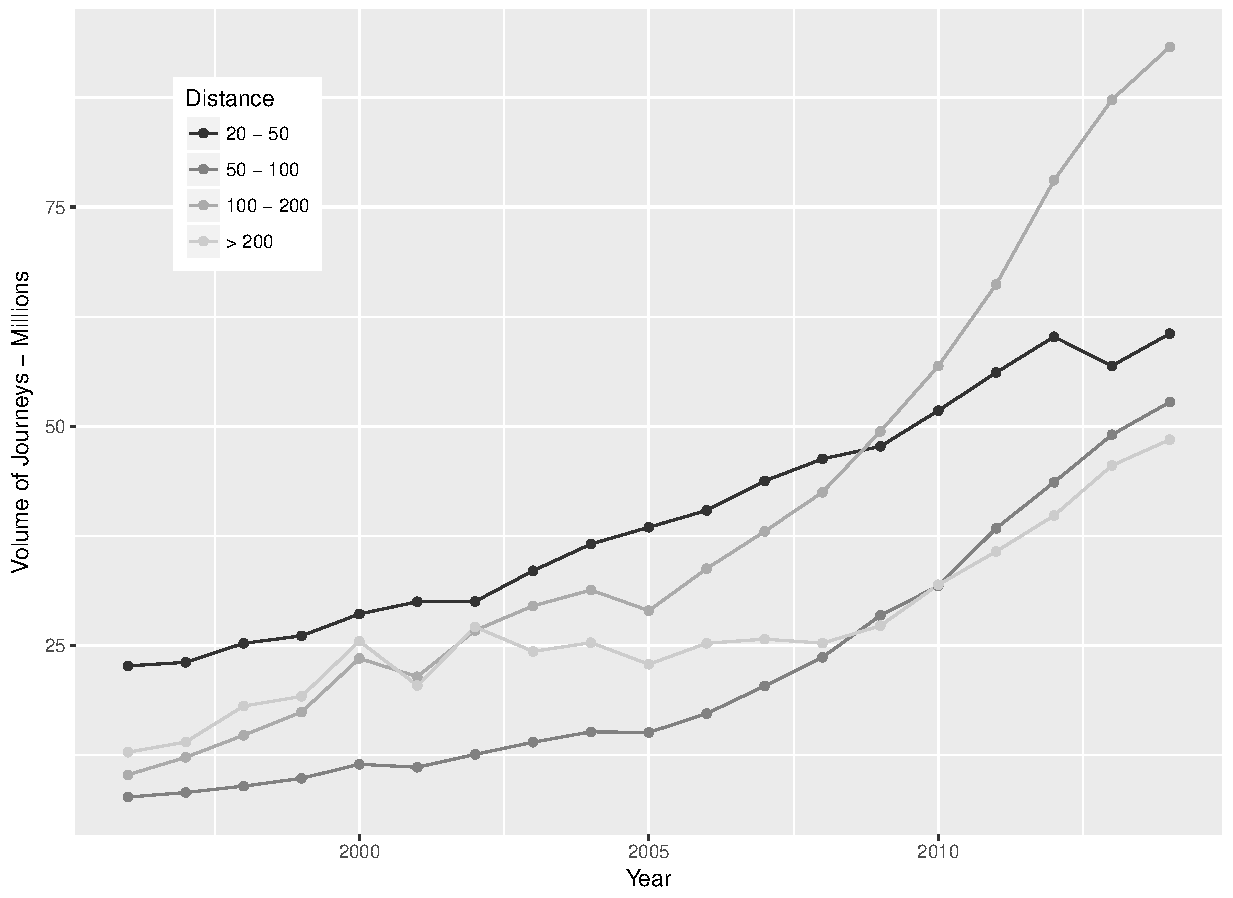
\includegraphics[width=\linewidth]{jny_growth}
  \caption{Growth of journeys per distance class}
  \label{fig:jny_growth}
\end{subfigure}

\caption{Explanatory Analysis on \textit{Journeys}}
\label{fig:jny}
\caption*{Source: Own work}
\end{figure}

\textit{Fares}

In which regards the variable \textit{fares}, Figure \ref{fig:bp_fares} illustrates the range of values in universe of fares for all routes (OD pairs) comprised in the dataset. To make them more comparable they were converted in pounds per mile.

The top row covers the first class fares, separated by type of fare - \textit{full}, \textit{reduced} and \textit{advance}. The bottow row refers to the standard class.

From these graphs one may notice that the range of \textit{full} fares is increasing over the time, both for first and standard class. The \textit{reduced} fare, in turn, shows a significantly smaller range in the standard class, whilst for the first class, it does not seem to follow a pattern. The restricted range of the standard reduced fares may be due to the ceiling imposed by regulation, as discussed in Chapter \ref{chp:lit-rev}.

Lastly, in which regards the \textit{advance} fares, which is a mix of discounted \textit{full} and \textit{reduced}, they present a steady median, slightly slower than the reduced fares but with a wider range in the standard class. For the first class, despite the lack o pattern for the \textit{reduced} fare, the advance also shows a steady median, lower than the \textit{full}, with a step change in the year 2000, which was also observed in the \textit{reduced}. 

\begin{figure}[H]
\centering
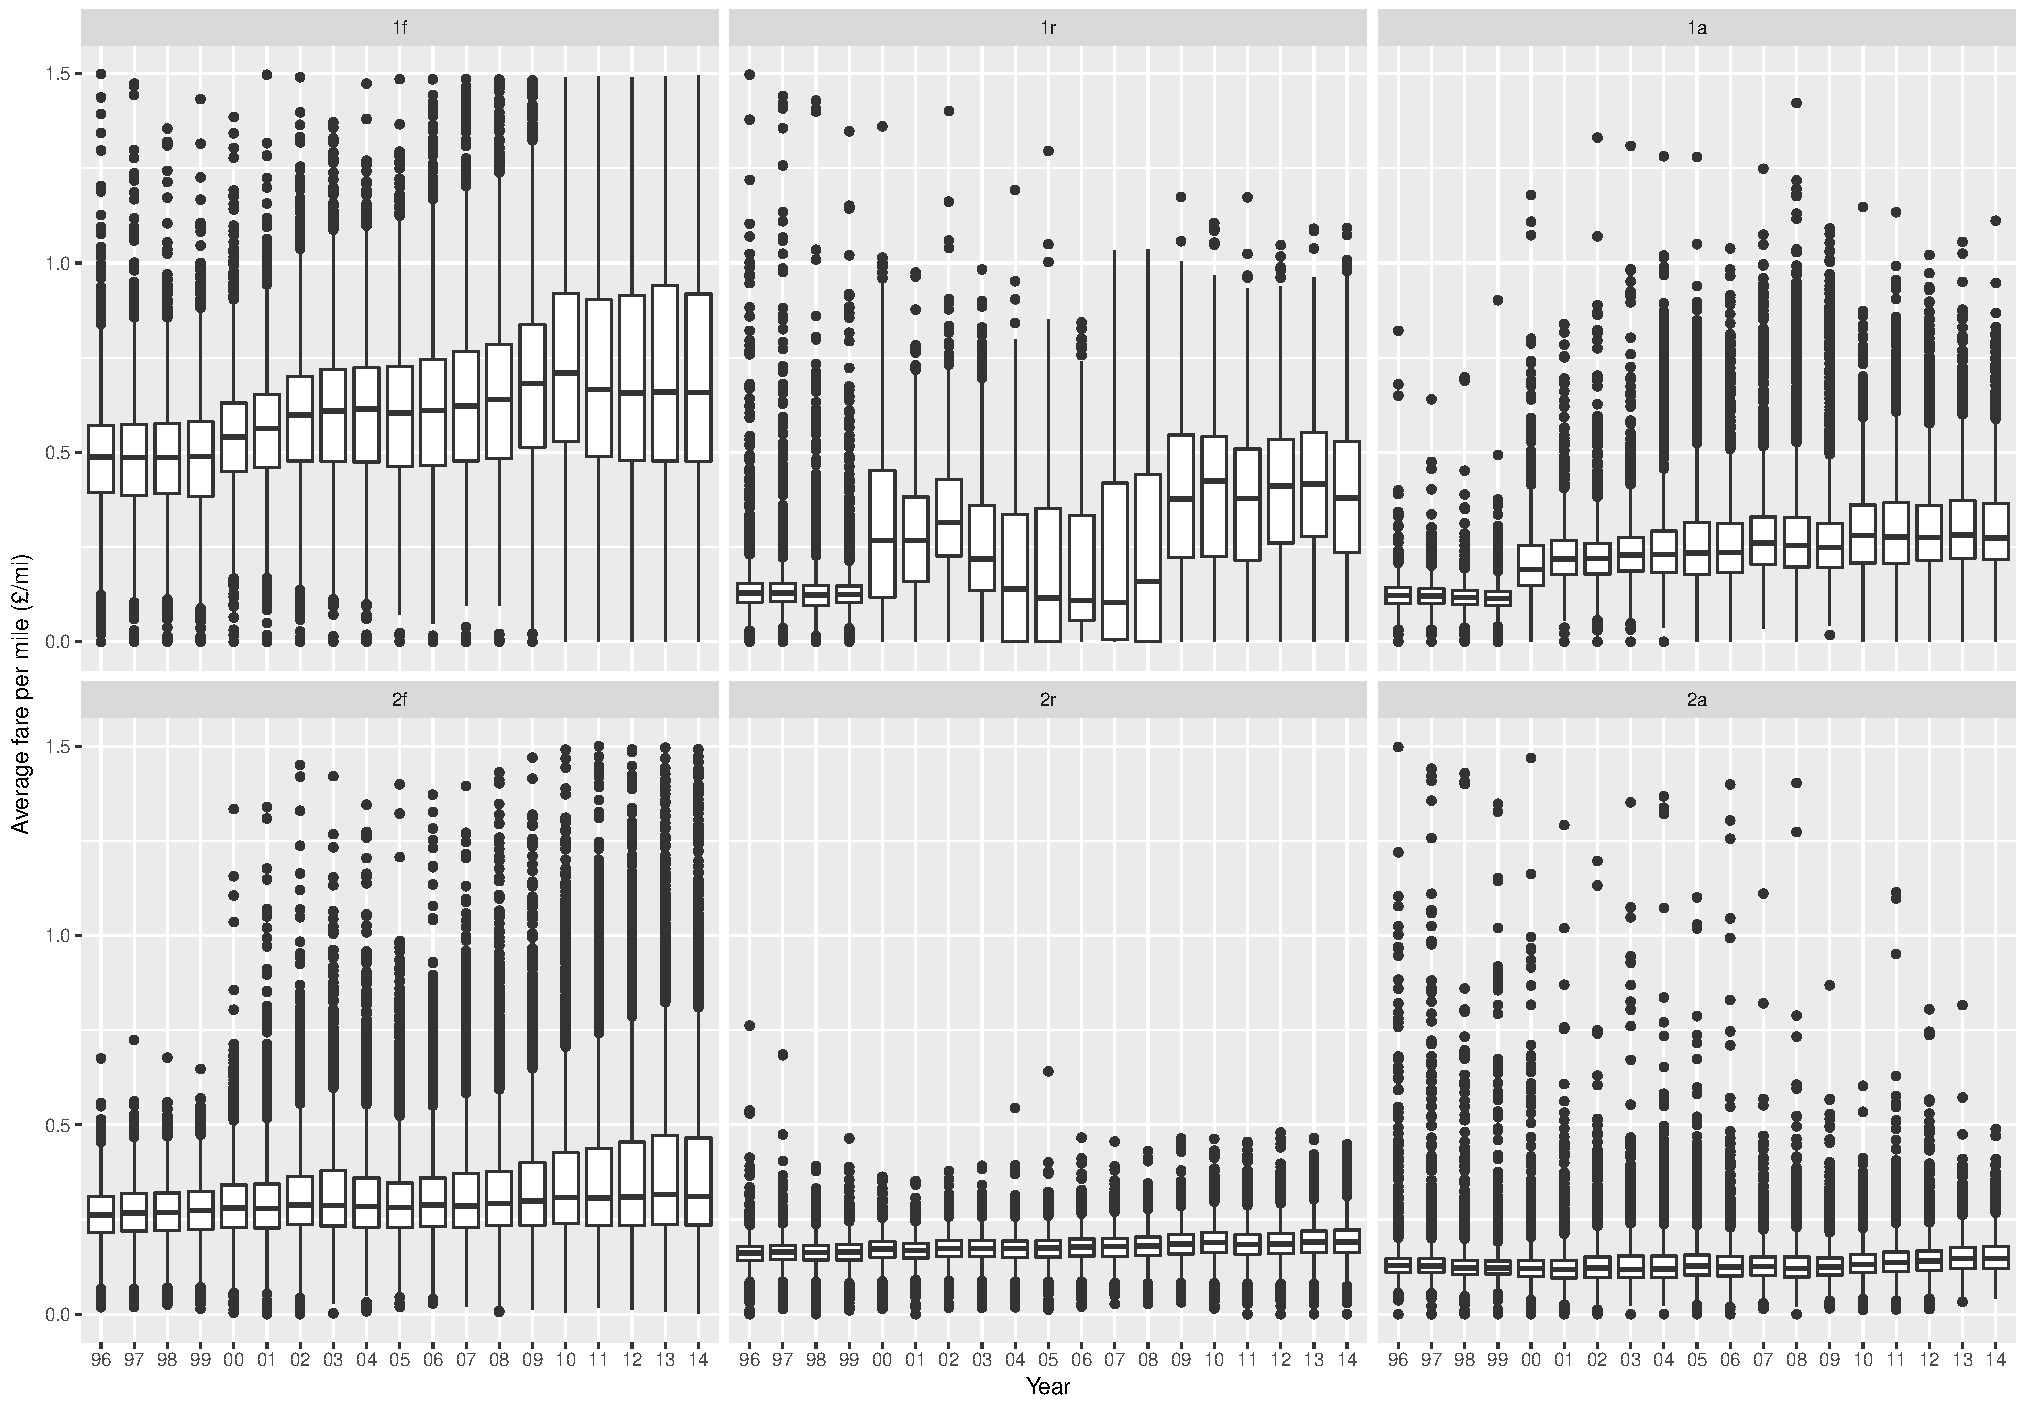
\includegraphics[width=\linewidth]{bp_fares}
\caption{Dispersion of fares per mile accross the OD pairs}
\label{fig:bp_fares}
\caption*{Source: Own work}
\end{figure} 

\textit{Gross Added Value - GVA}

The GVA is a metric for the level of economic activity in a given region. Because rail demand is expected to have a positive polarity with economic activity \citep{pdfh} - the higher GVA, the higher volume of journeys - it is interesting to check this dynamic on the data.

To visualise it, the variable GVA was segmented in four levels. For each level, the average volume of journeys was calculated per year. As shown in Figure \ref{fig:gva_jny}, the higher the GVA level, the higher the average volume of journeys per route. Also, it is possible to notice an overall trend of growth of journeys for all levels of GVA. 

To complement the visualization, Figure \ref{fig:gva_od} brings more information about the range of GVA among the ODs pairs and how was the dynamic across the years. Because the OD pairs in the dataset remained constant over the years, with very few exceptions, one can notice that, in general terms, there was a trend towards the right. That means that regions are escalating to levels of higher economic activity. 

For the lowest level of GVA, at the left, it seems that have occurred a concentration movement which peaks very close to the boundary of the next level. Eventually, these OD pairs may have changed to next level of GVA. Also, the second and third levels seem to have spread towards the right. Lastly, the highest level of GVA appeared only in the year 2000 and seems to have a mild movement of expansion and contraction.

\begin{figure}[H]
\centering
\begin{subfigure}{.5\textwidth}
  \centering
  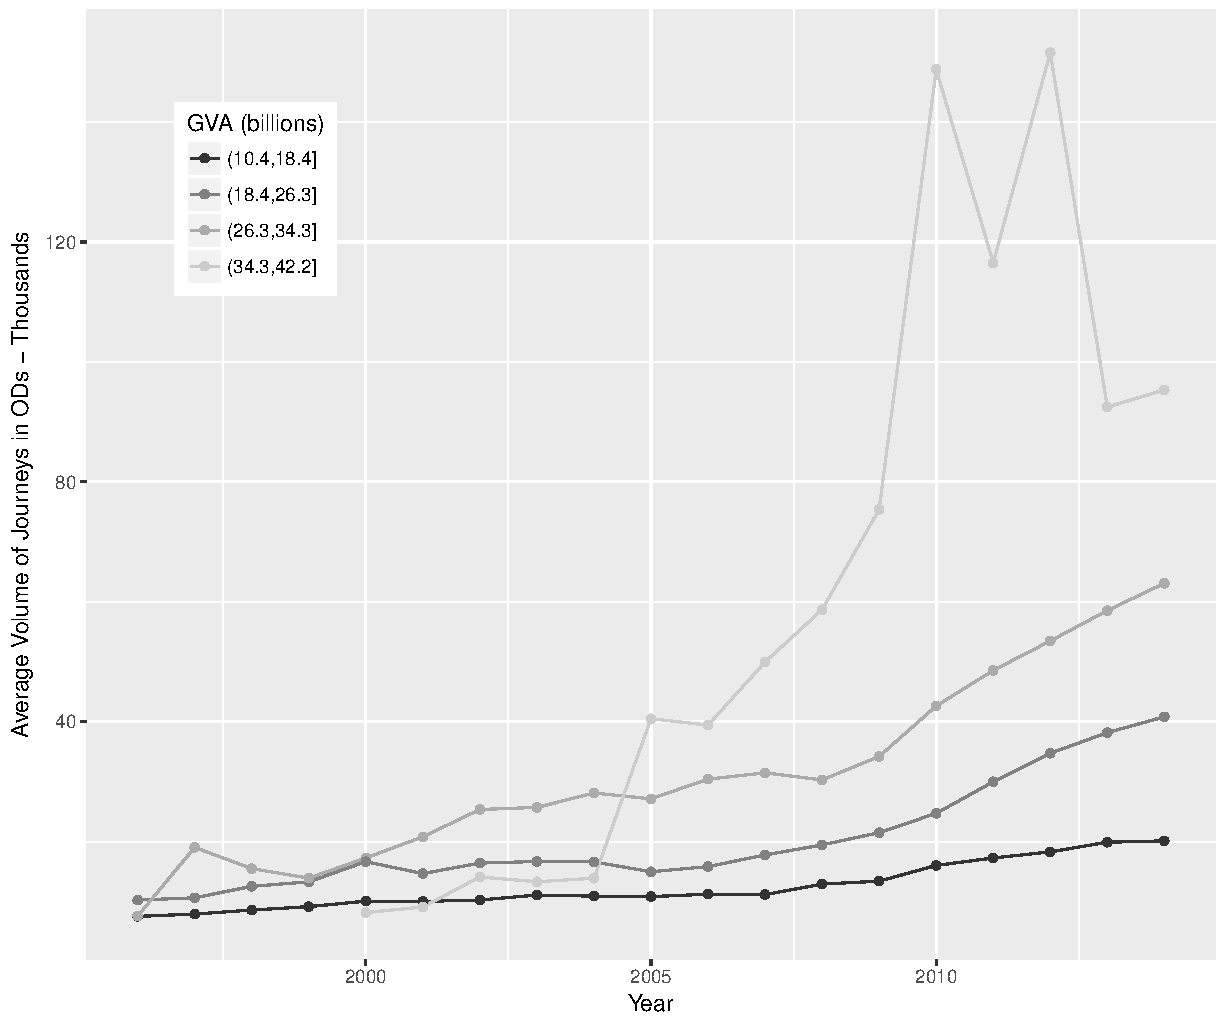
\includegraphics[width=\linewidth]{gva_jny}
  \caption{Growth journeys by level of GVA}
  \label{fig:gva_jny}
\end{subfigure}%
\begin{subfigure}{.5\textwidth}
  \centering
  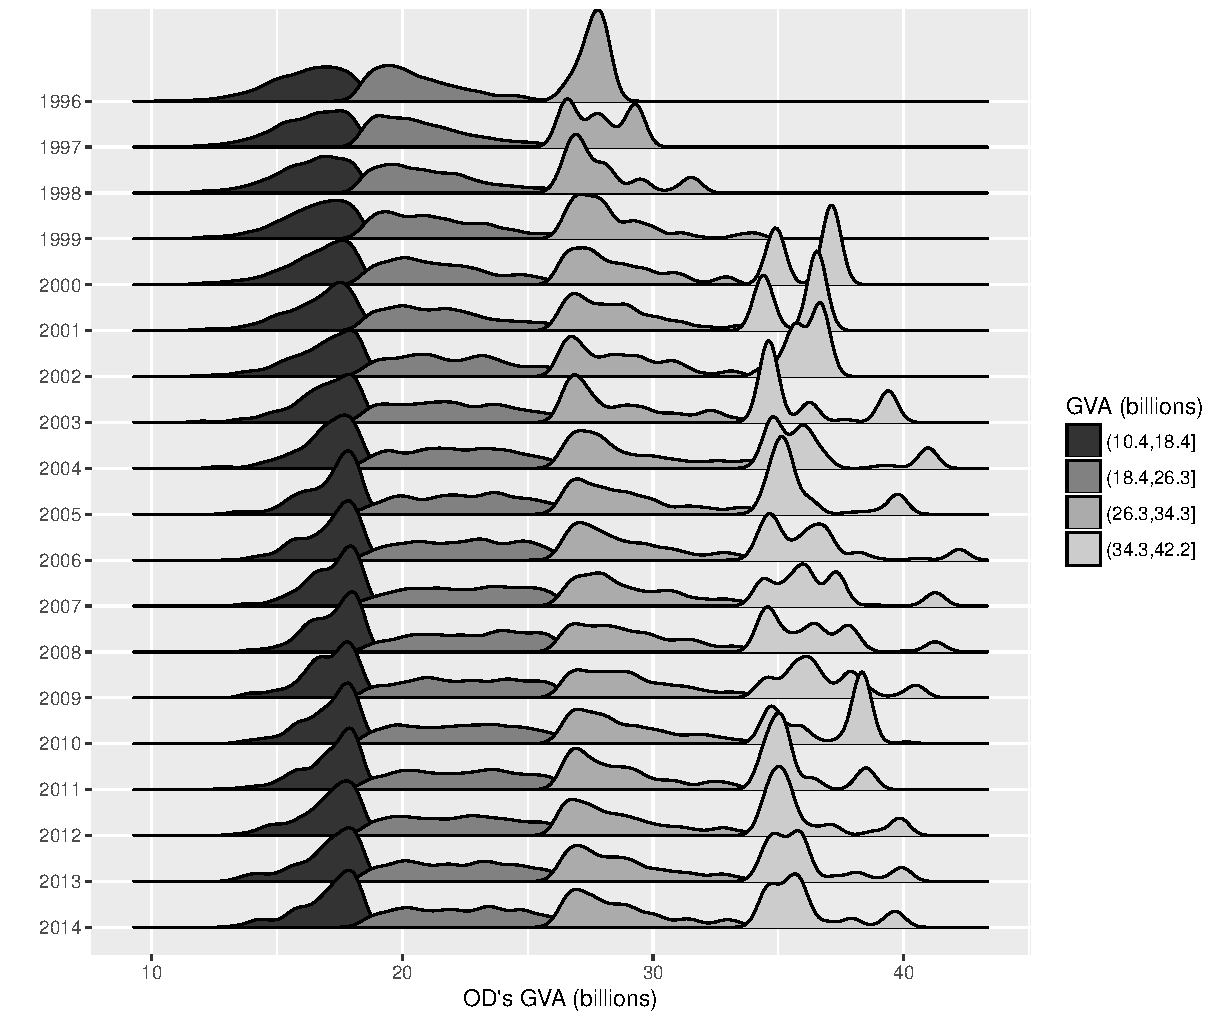
\includegraphics[width=\linewidth]{gva_od}
  \caption{Distribution of OD pairs' GVA}
  \label{fig:gva_od}
\end{subfigure}%
\caption{Exploratory Analysis on \textit{GVA}}
\label{fig:gva}
\caption*{Source: Own work}
\end{figure}

In short, eyeballing the \textit{GVA} variable it is possible to identify consistency between the theoretical relation of economic activity and rail journeys in the data.
\\[3pt]

% \begin{figure}[H]
% \centering
% \begin{subfigure}{.5\textwidth}
%   \centering
%   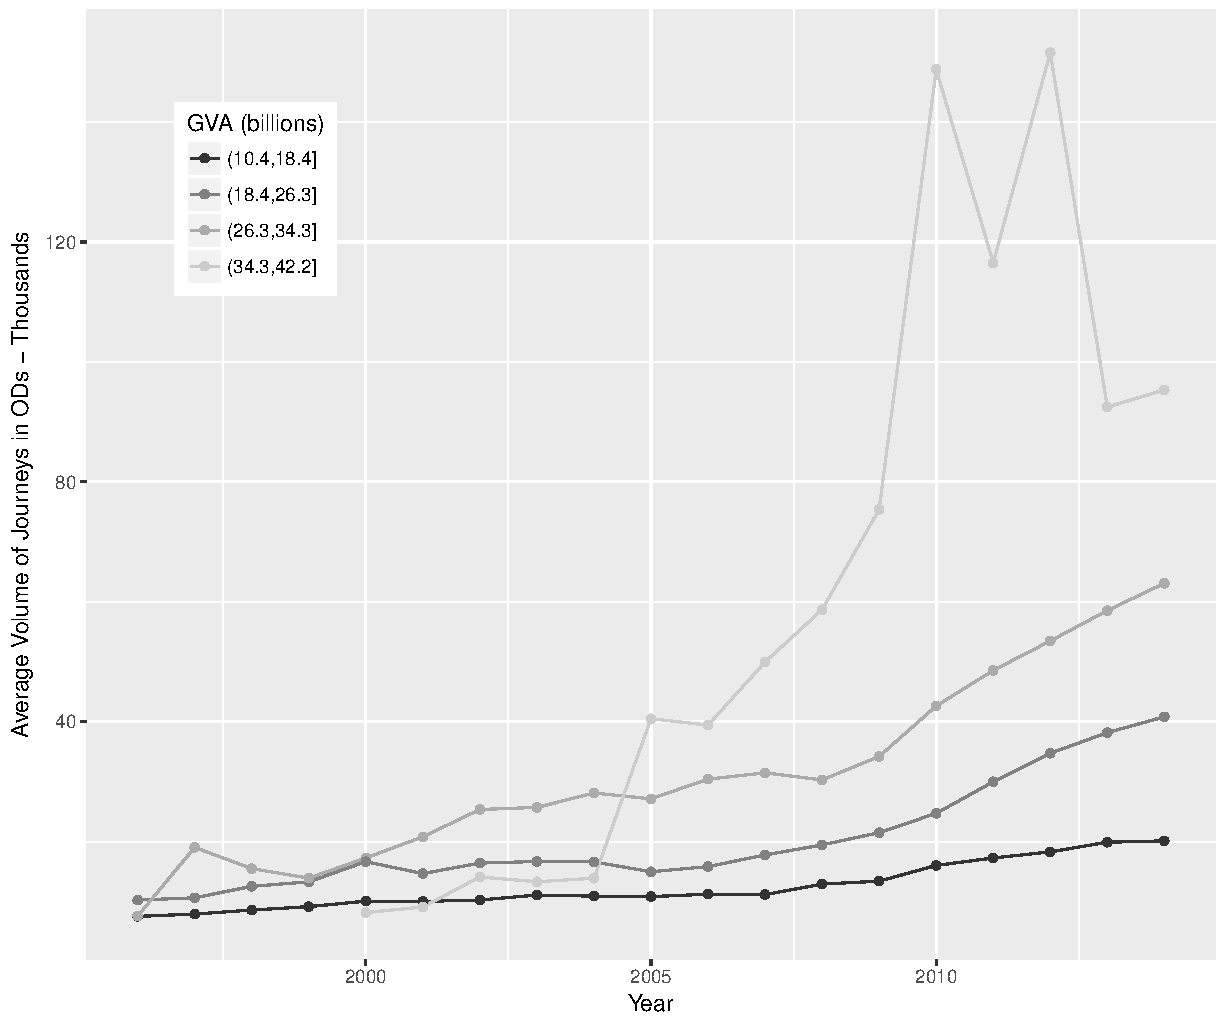
\includegraphics[width=\linewidth]{gva_jny}
%   \caption{Growth journeys by level of GVA}
%   \label{fig:gva_jny}
% \end{subfigure}%
% \begin{subfigure}{.4\textwidth}
%   \centering
%   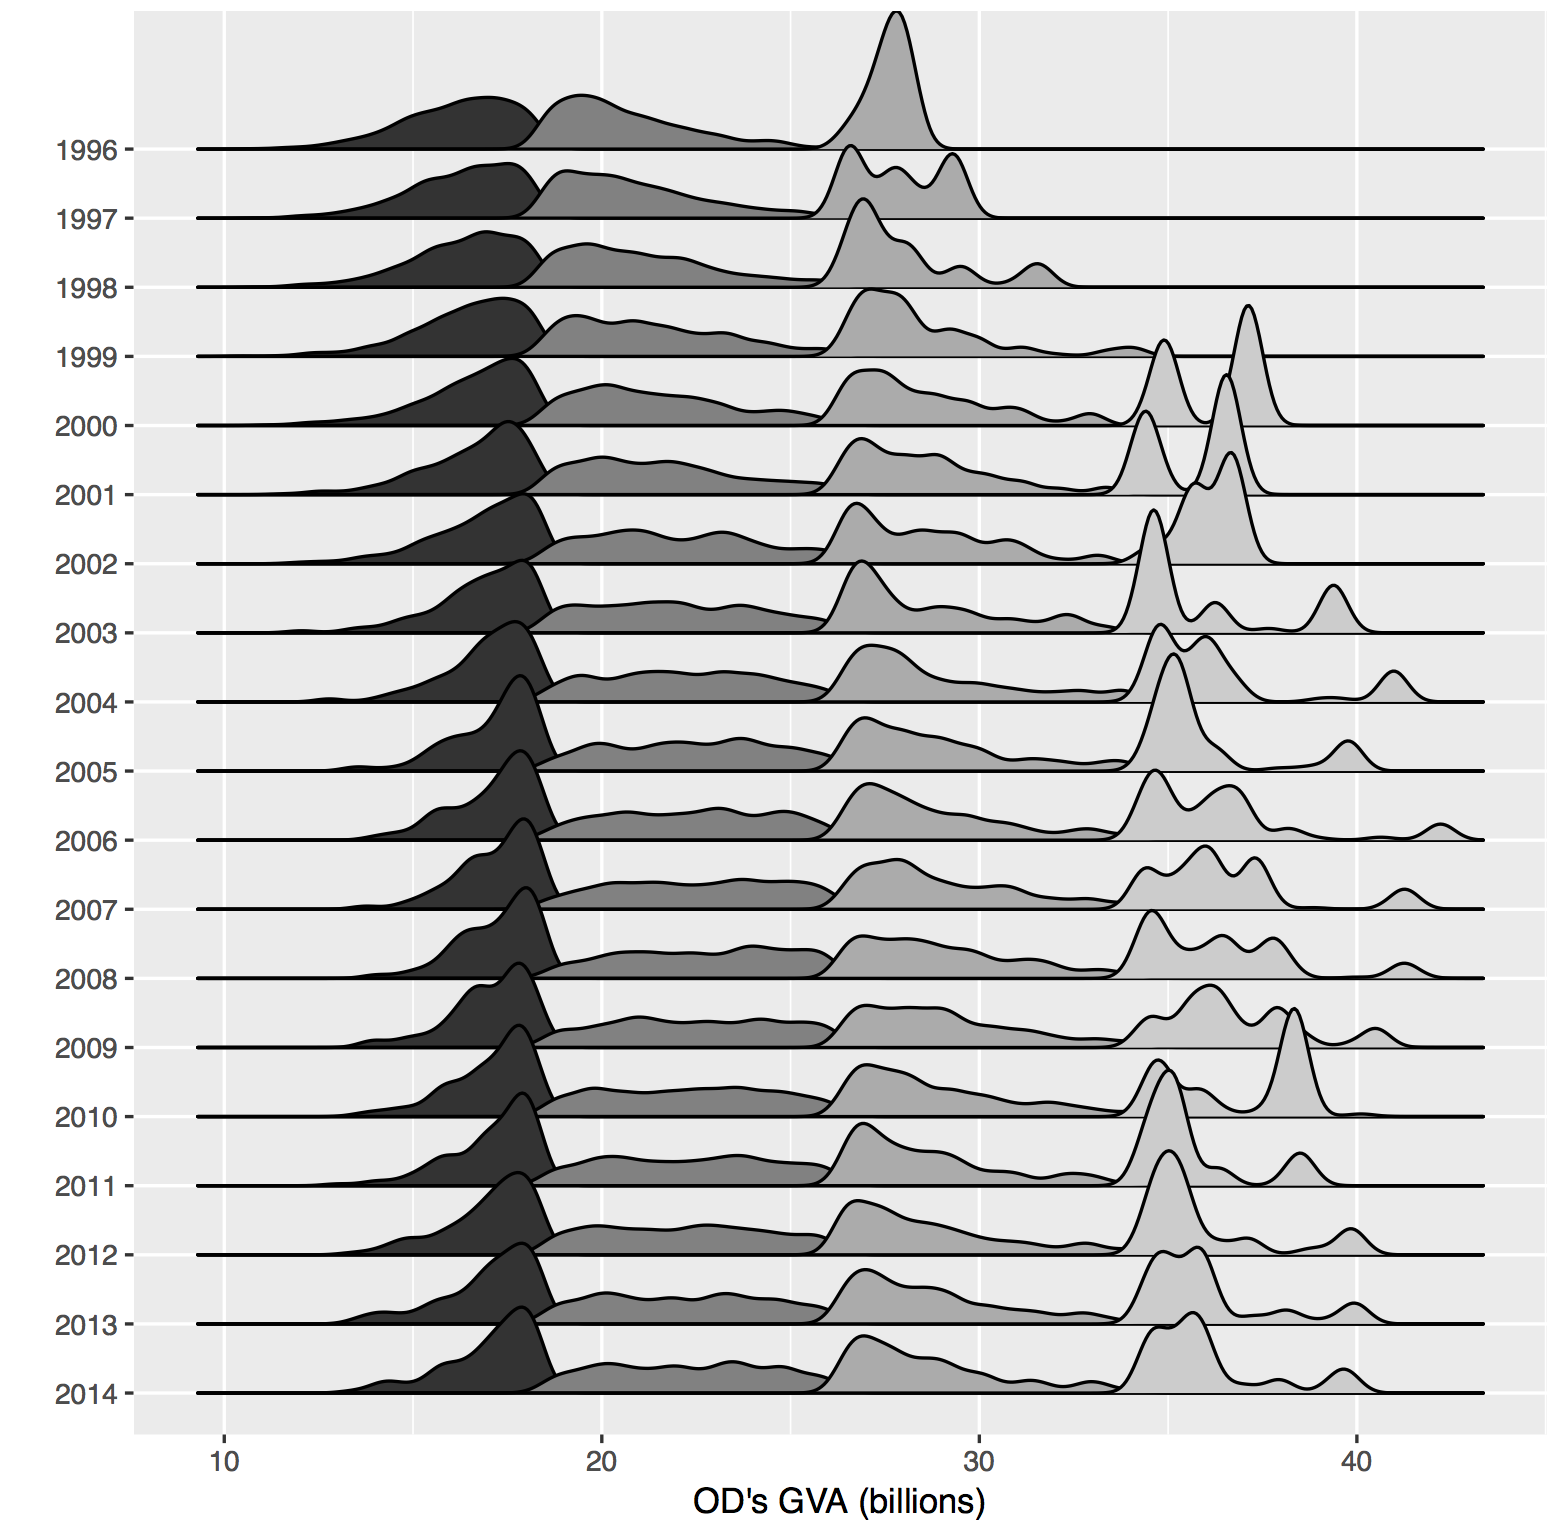
\includegraphics[width=\linewidth]{gva_od1}
%   \caption{Distribution of OD pairs' GVA}
%   \label{fig:gva_od}
% \end{subfigure}%
% \begin{subfigure}{.2\textwidth}
%   \centering
%   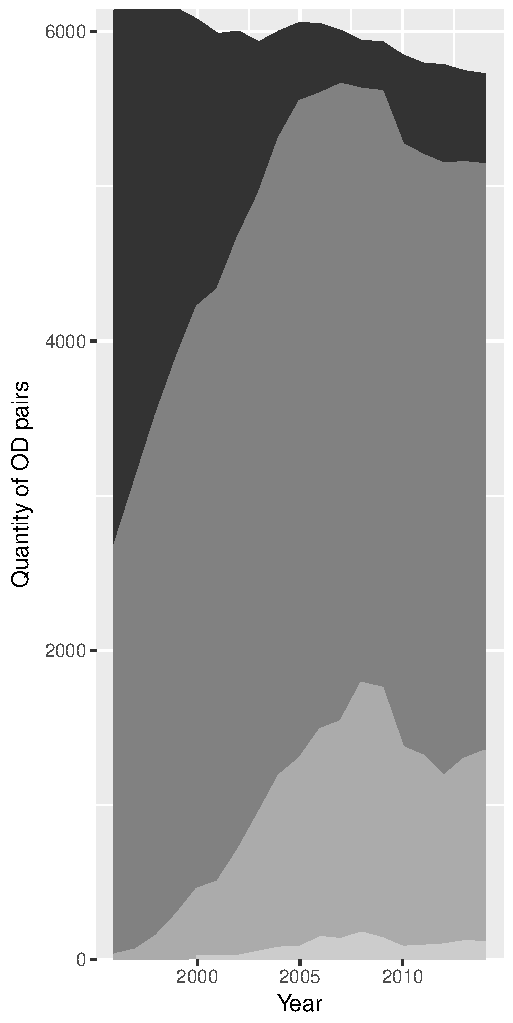
\includegraphics[width=\linewidth]{od}
%   \caption{OD pairs by GVA}
%   \label{fig:d}
% \end{subfigure}%
% \caption{Explanatory Analysis on \textit{GVA}}
% \label{fig:gva}
% \caption*{Source: Own elaboration}
% \end{figure}


\textit{Generalised Journey Time - GJT}

In this work, the GJT measure represents the quality-related drivers of demand. It comprises the journey time plus the frequency and interchange penalties, as defined in PDFH, and it is measured in minutes.

To understand the dynamics of this variable Figure \ref{fig:gjt} brings two dimensions of it: an overview of the GJT of the OD pairs considered in the study and the accumulated average reduction of GJT over the years, taking the year 1996 as the base.

Figure \ref{fig:gjt_hist} shows the overall distribution of routes by GJT. As a general characterization, it is possible to observe that the mass of routes peaks around 150 minutes and decreases as the GJT increases, achieving extreme values over 1,000 minutes. 

Additionally, Figure \ref{fig:gjt_years} shows how, in average, routes are reducing their GJT over the years. The values plotted in the graph are accumulated reductions with respect to the year 1996. It is observed an average reduction of 7.3\% in the GJT in 19 years (1996-2014).

\begin{figure}[H]
\centering
\begin{subfigure}{.5\textwidth}
  \centering
  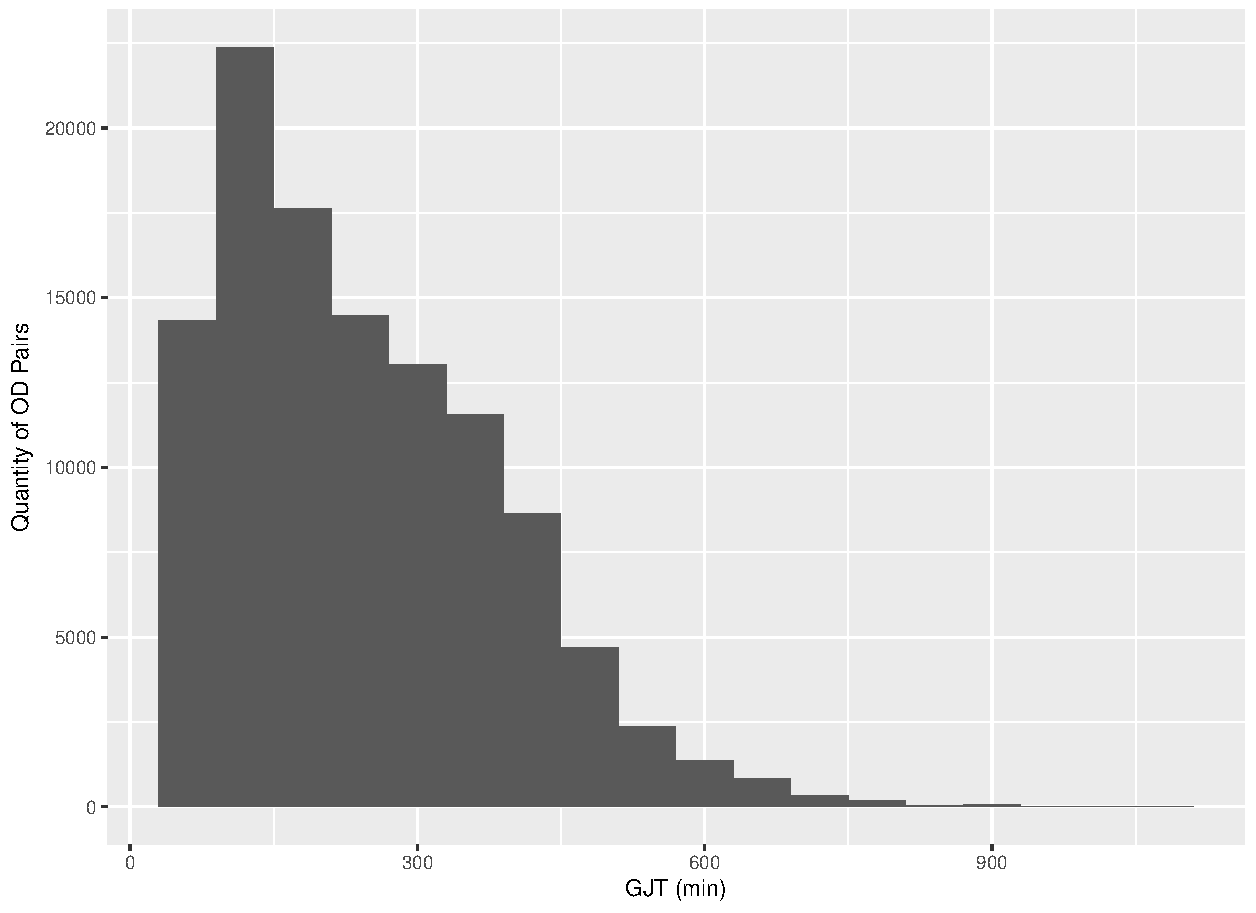
\includegraphics[width=\linewidth]{gjt_hist}
  \caption{Distribution of GJT across the routes}
  \label{fig:gjt_hist}
\end{subfigure}%
\begin{subfigure}{.5\textwidth}
  \centering
  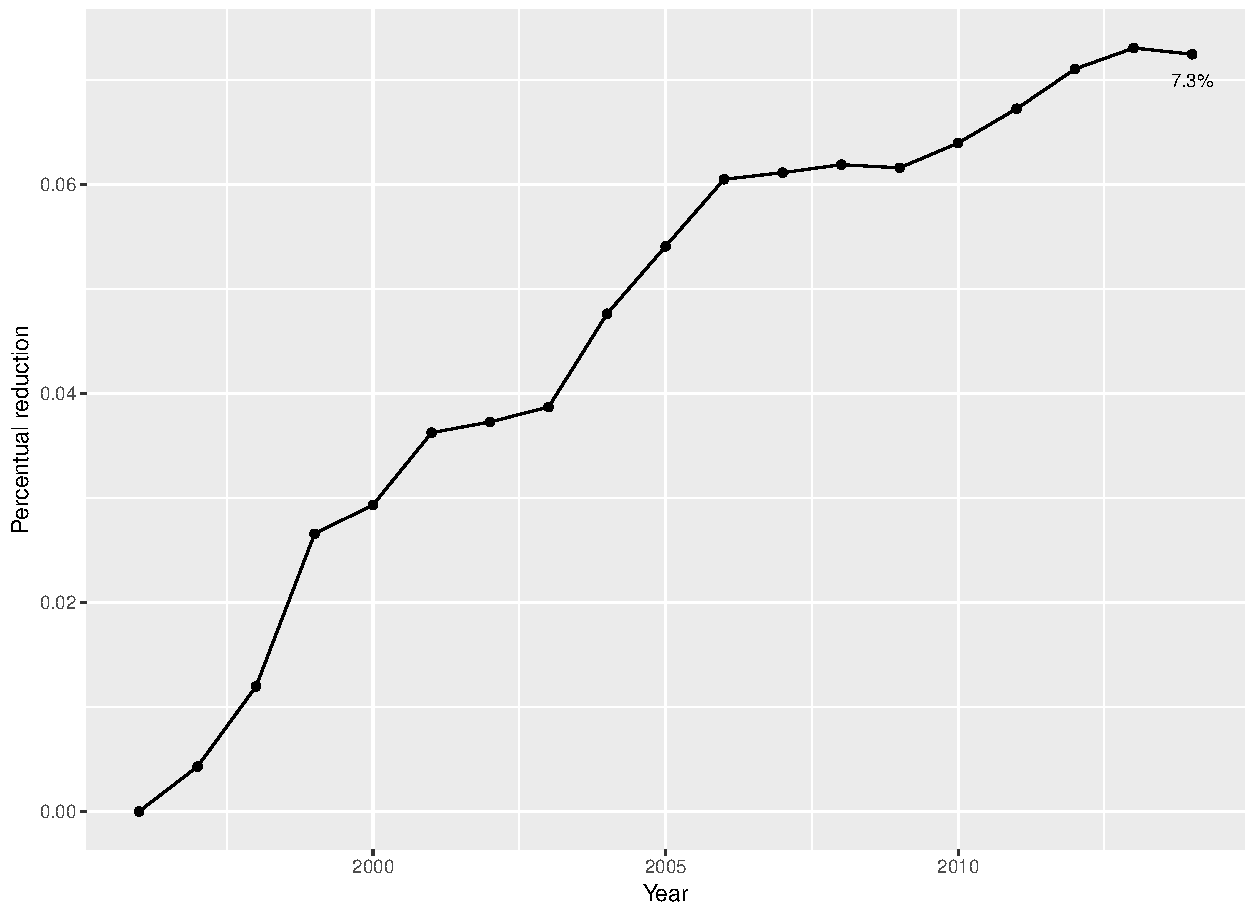
\includegraphics[width=\linewidth]{gjt_years}
  \caption{Accumulated Reduction of GJT}
  \label{fig:gjt_years}
\end{subfigure}%
\caption{Exploratory Analysis on \textit{GJT}}
\label{fig:gjt}
\caption*{Source: Own work}
\end{figure}

\subsection{Subsetting markets in the dataset}

The availability or not of a different set of tickets across the routes creates different markets environments. When there are more types of fares the competition increases and the market share of tickets is affected simply because there are more options at one's disposal. 

% For instance, a big player is the first class tickets.

Therefore, the existence of different sets of fares in a route affects the fare elasticities. For example, the fare elasticity of reduced tickets with respect to the demand for full tickets may differ whether there is or not the first class ticket.

The dataset was subsetted into four markets to properly estimate the fare elasticities for each circumstance. The two first will regard only the standard class, and in the other two, first class will be added. 

With the introduction of first class tickets in the Markets 3 and 4, their complexity has increased significantly. To overcome that, the coverage of the dataset was shortened to a regional level to reduce the unobserved heterogeneity and provide a more well-behaved data. The regions \footnote{NUTS 1 level regions.} chosen were Scotland and Yorkshire and Humber, so only routes which both origin and destination in these regions were considered. There was no strong justification for choosing these regions beyond the fact that any interference with London flows was avoided.

An alternative to keep the broad coverage and reduce the heterogeneity that may exist across regions could be the adoption of dummy variables to capture these unobserved characteristics. However, this option was not adopted because in the Bayesian framework it would represent an increase of 10 marginal posterior distributions (from the 11 regions), in each regression model. It was considered, thus, that such complexity was needless since this is an introductory study of Bayesian econometrics in the field. It is important to be aware, however, that a cut in the dataset is a stronger isolation of unobserved characteristics than regressing with dummy variables. 

Table \ref{tbl:market_subs} presents summary information on the resultant dataset for each market.


\begin{table}[H] \centering 
  \caption{Market subsetting} 
  \label{tbl:market_subs} 
{\renewcommand\arraystretch{1.25}}
\begin{tabular} {cccccc}
\toprule
Market             & Fares      & OD Pairs & Time Series & Obs  & Coverage\\
\hline
1                  & 2F, 2R         & 2,074     & 1996 - 2014   & 15,481 & Great Britain\\
\hline
2                  & 2F, 2R, 2A     & 1,550     & 2000 - 2014 & 5,909  & Great Britain\\
\hline
\multirow{2}{*}{3} & 1N, 2F, 2R,  & \multirow{2}{*}{516} & \multirow{2}{*}{1996 - 2014} & \multirow{2}{*}{5,783} & Scotland - Yorkshire \\
                   &   2A         &                      &                              &                        & and Humber\\
\hline
\multirow{2}{*}{4} & 1F, 1R, 1A,& \multirow{2}{*}{251} & \multirow{2}{*}{1996 - 2014} & \multirow{2}{*}{1,738} & Scotland - Yorkshire \\ 
				   & 2F, 2R, 2A &                        &                              &                      & and Humber\\
\bottomrule
\end{tabular}%
\caption*{Source: Own work}
\end{table} 



It should not be expected, however, that the quantity of OD pairs shown in Table \ref{tbl:market_subs} to be constant over the years because the availability of tickets for a given route is not fixed in time. It may happen that the quantity of ODs pairs in each market varies from year to year. For example, if in a given route the first class ticket started being commercialised in the year 2000 onwards, this OD pair was considered in market 1 or 2 before 2000 and in market 3 or 4 after that. The important is that the pool of each market is coherent with their actual competition conditions. For completeness, Figure \ref{fig:od_mkts} illustrates the variation of OD pairs in each market.

\begin{figure}[H]
\centering
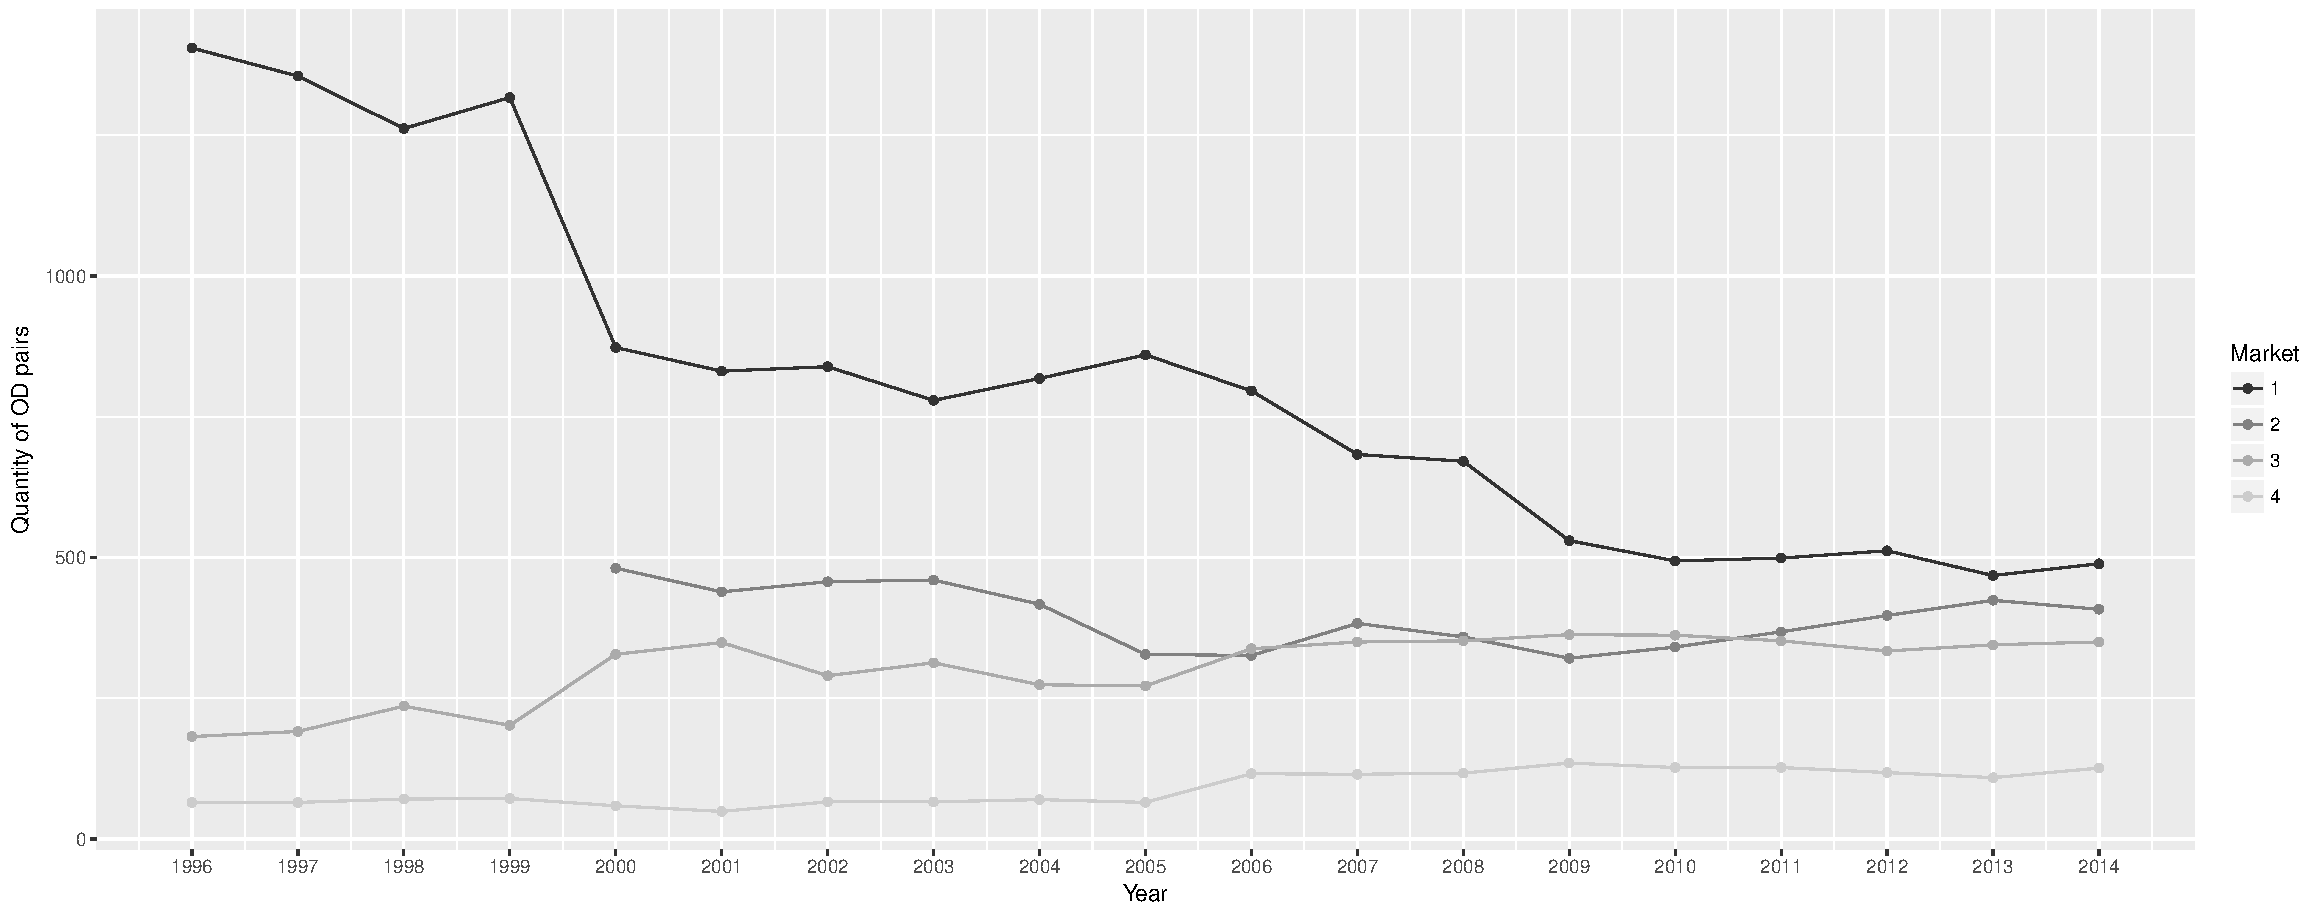
\includegraphics[width=\linewidth]{od_mkt.pdf}
\caption{Quantity of OD pairs by market along the years}
\label{fig:od_mkts}
\caption*{Source: Own work}
\end{figure} 

Another aspect that may be relevant to analyse the results is the market share of fares. Table \ref{tbl:mktshr} shows these numbers.

It is noticeable that in all markets the dominance of the \textit{standard reduced} fare, followed by the \textit{standard full}. It is also noticeable that the \textit{advance} ticket has been gaining space, growing from 1\% to 8\% in 15 years, in Market 2, and from 4\% to 12\% in Market 3. The \textit{first class} tickets presented a small market share, in decline in both Markets 3 and 4, from 7\% to 3\% and 5-6\% to 2-0\%, respectively. It is observable that the \textit{First Class} tickets when disaggregated by fare type show very small market shares, even less than 1\%.

\begin{landscape}

\begin{table}[!ht] \centering 
  \caption{Market share of fares by market segmentation} 
  \label{tbl:mktshr} 
{\renewcommand\arraystretch{1.25}}
\begin{tabular} {cccccccccccccccccccc}
  \toprule
  &\multicolumn{2}{c}{Market 1} & & \multicolumn{3}{c}{Market 2} & & \multicolumn{4}{c}{Market 3} & & \multicolumn{6}{c}{Market 4} \\
 \cline{2-3} \cline{5-7} \cline{9-12} \cline{14-19} 
 Year & 2F  & 2R   & & 2F   & 2R   & 2A  & & 1N  & 2F   & 2R   & 2A   & & 1F & 1R & 1A & 2F & 2R & 2A \\ 
  \hline
1996 & 41\% & 59\% & & -    & -    & -   & & 7\% & 28\% & 61\% & 4\%  & & 5\% & 5\% & 6\% & 7\%  & 66\% & 11\% \\ 
1997 & 39\% & 61\% & & -    & -    & -   & & 7\% & 32\% & 55\% & 6\%  & & 4\% & 9\% & 6\% & 7\%  & 60\% & 15\% \\ 
1998 & 38\% & 62\% & & -    & -    & -   & & 7\% & 31\% & 57\% & 5\%  & & 4\% & 8\% & 5\% & 12\% & 58\% & 13\% \\ 
1999 & 37\% & 63\% & & -    & -    & -   & & 9\% & 26\% & 58\% & 7\%  & & 5\% & 8\% & 6\% & 7\%  & 59\% & 15\% \\ 
2000 & 39\% & 61\% & & 26\% & 73\% & 1\% & & 2\% & 34\% & 58\% & 6\%  & & 4\% & 0\% & 0\% & 26\% & 58\% & 11\% \\ 
2001 & 38\% & 62\% & & 31\% & 68\% & 1\% & & 2\% & 34\% & 59\% & 5\%  & & 4\% & 0\% & 0\% & 27\% & 60\% &  8\% \\ 
2002 & 39\% & 61\% & & 25\% & 73\% & 2\% & & 3\% & 32\% & 59\% & 6\%  & & 4\% & 0\% & 0\% & 26\% & 60\% & 10\% \\ 
2003 & 38\% & 62\% & & 33\% & 66\% & 1\% & & 2\% & 28\% & 64\% & 6\%  & & 3\% & 0\% & 0\% & 21\% & 65\% & 10\% \\ 
2004 & 39\% & 61\% & & 32\% & 67\% & 1\% & & 3\% & 26\% & 64\% & 8\%  & & 3\% & 0\% & 1\% & 17\% & 68\% & 11\% \\ 
2005 & 38\% & 62\% & & 32\% & 66\% & 2\% & & 2\% & 25\% & 67\% & 6\%  & & 3\% & 0\% & 1\% & 17\% & 68\% & 11\% \\ 
2006 & 38\% & 62\% & & 35\% & 62\% & 2\% & & 2\% & 27\% & 64\% & 6\%  & & 3\% & 0\% & 1\% & 21\% & 65\% & 11\% \\ 
2007 & 38\% & 62\% & & 38\% & 60\% & 2\% & & 2\% & 31\% & 62\% & 5\%  & & 3\% & 0\% & 1\% & 23\% & 61\% & 11\% \\ 
2008 & 39\% & 61\% & & 36\% & 61\% & 3\% & & 3\% & 31\% & 62\% & 4\%  & & 3\% & 0\% & 1\% & 26\% & 62\% &  8\% \\ 
2009 & 43\% & 57\% & & 38\% & 59\% & 3\% & & 3\% & 29\% & 59\% & 8\%  & & 3\% & 2\% & 1\% & 25\% & 57\% & 12\% \\ 
2010 & 43\% & 57\% & & 38\% & 58\% & 4\% & & 3\% & 26\% & 63\% & 8\%  & & 2\% & 1\% & 1\% & 20\% & 64\% & 12\% \\ 
2011 & 45\% & 55\% & & 40\% & 56\% & 4\% & & 3\% & 26\% & 62\% & 9\%  & & 1\% & 1\% & 1\% & 20\% & 63\% & 13\% \\ 
2012 & 47\% & 53\% & & 38\% & 56\% & 6\% & & 3\% & 23\% & 65\% & 9\%  & & 1\% & 1\% & 1\% & 16\% & 68\% & 12\% \\ 
2013 & 46\% & 54\% & & 35\% & 58\% & 6\% & & 3\% & 31\% & 55\% & 12\% & & 2\% & 0\% & 2\% & 28\% & 49\% & 19\% \\ 
2014 & 43\% & 57\% & & 37\% & 55\% & 8\% & & 3\% & 33\% & 52\% & 12\% & & 2\% & 0\% & 2\% & 28\% & 48\% & 20\% \\
   \bottomrule
\end{tabular}
\caption*{Source: Own work}
\end{table}

\end{landscape}

\subsection{Data correlation}

As mentioned in Chapter \ref{chp:lit-rev}, the correlation has been a problem in the previous studies in fares elasticities estimation.

Checking the data used in this study, it is noticed that correlation is also present, as should be expected. Figure \ref{fig:cor} presents correlation matrixes of the fares variables for each market after the segmentation of the dataset.

\begin{figure}[H]
\centering
\begin{subfigure}{.5\textwidth}
  \centering
  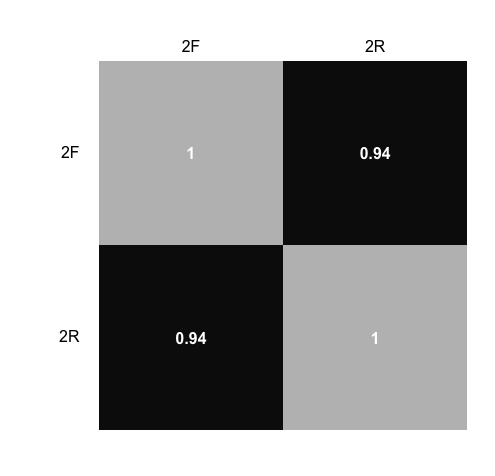
\includegraphics[width=\linewidth]{cor_mkt41}
  \caption{Market 1}
  \label{fig:cor_mkt4}
\end{subfigure}%
\begin{subfigure}{.5\textwidth}
  \centering
  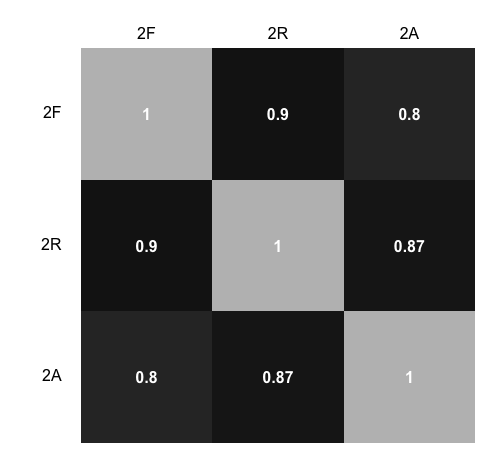
\includegraphics[width=\linewidth]{cor_mkt21}
  \caption{Market 2}
  \label{fig:cor_mkt2}
\end{subfigure}%

\begin{subfigure}{.5\textwidth}
  \centering
  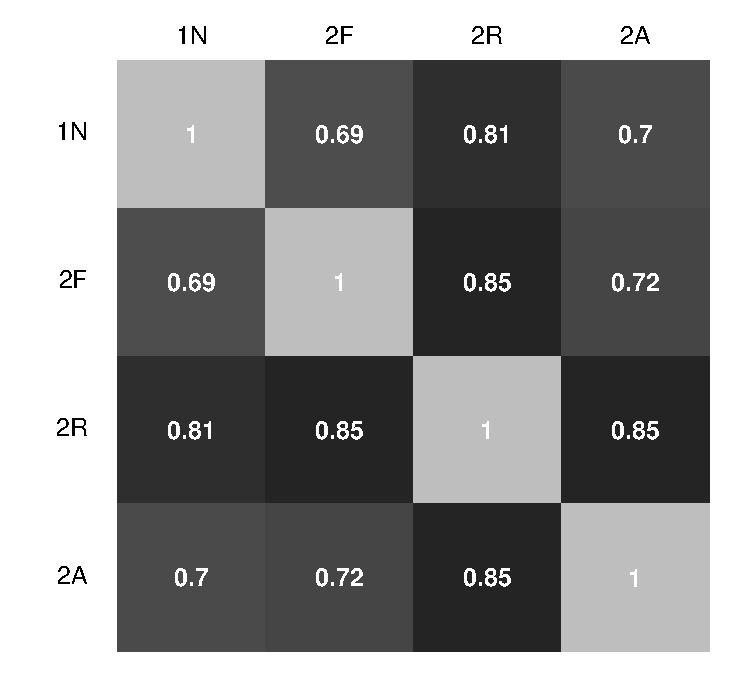
\includegraphics[width=\linewidth]{cor_mkt3_SCOTYORK}
  \caption{Market 3}
  \label{fig:cor_mkt3}
  \end{subfigure}%
\begin{subfigure}{.5\textwidth}
  \centering
  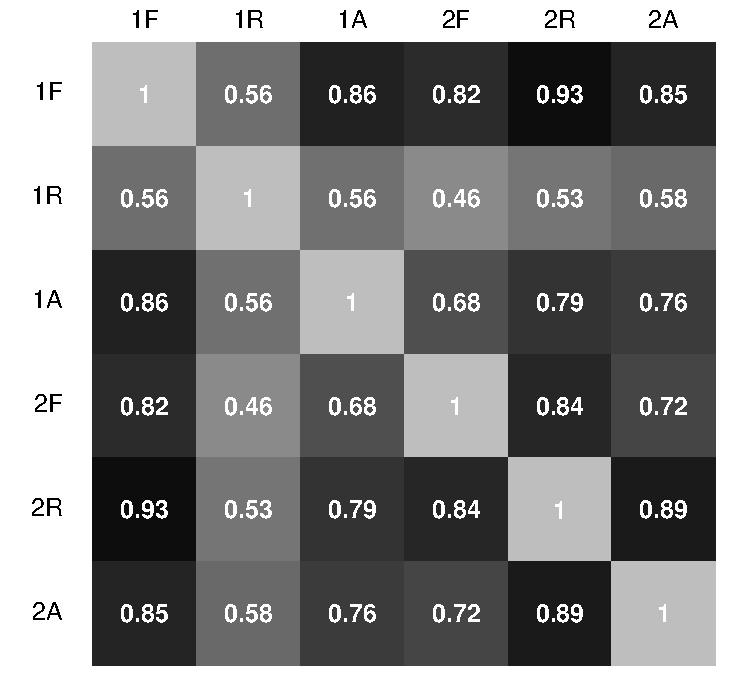
\includegraphics[width=\linewidth]{cor_mkt4_SCOTYORK}
  \caption{Market 4}
  \label{fig:cor_mkt1}
\end{subfigure}%
\caption{Correlation of fares by market}
\label{fig:cor}
\caption*{Source: Own work}
\end{figure}

In Market 1, there is a high correlation between fares, computed as $0.94$. Also for the Market 2 the correlations are still very high, above of $0.80$. For Market 3, correlation assumes lower values, but still for the \textit{reduced} and \textit{advance}, and \textit{reduced} and \textit{full} tickets of the standard class they are very high, deemed as $0.85$ for both. For Market 4, correlations above $0.80$ for two-fifths of the coefficients.

Despite the presence of high correlation among the fares, it should not be an issue in Bayesian regression when strong informative priors are provided, as discussed in Chapter \ref{chp:lit-rev}. 

 % Despite the bayesian approach does not overcomer this issue, it has a different way to deal with it, as discussed previously in Chapter \ref{chp:lit-rev}. It is important, therefore, to idenfity the extension of correlation in the data to be aware of it when stablishing the priors and interpreting the results. 

\section{Model}
% 400 words

Bayesian models are usually wrote formally as shown in Equation \ref{eq:model}. This format is useful to identify the elements that must conceptualised when building a model: the linear model, the likelihood, and the priors. Next subsections will work on these elements.

% In order to conceptualize a model, \cite{mcelreath2012} presents a useful framework especially for bayesian methods, even though it can be expanded for all kind of techniques. This scheme is a sequence of decision that helps to identify the elements of the model. Figure \ref{fig:model_decision_framework} illustrates it.

% \begin{figure}[H]
% \centering
% 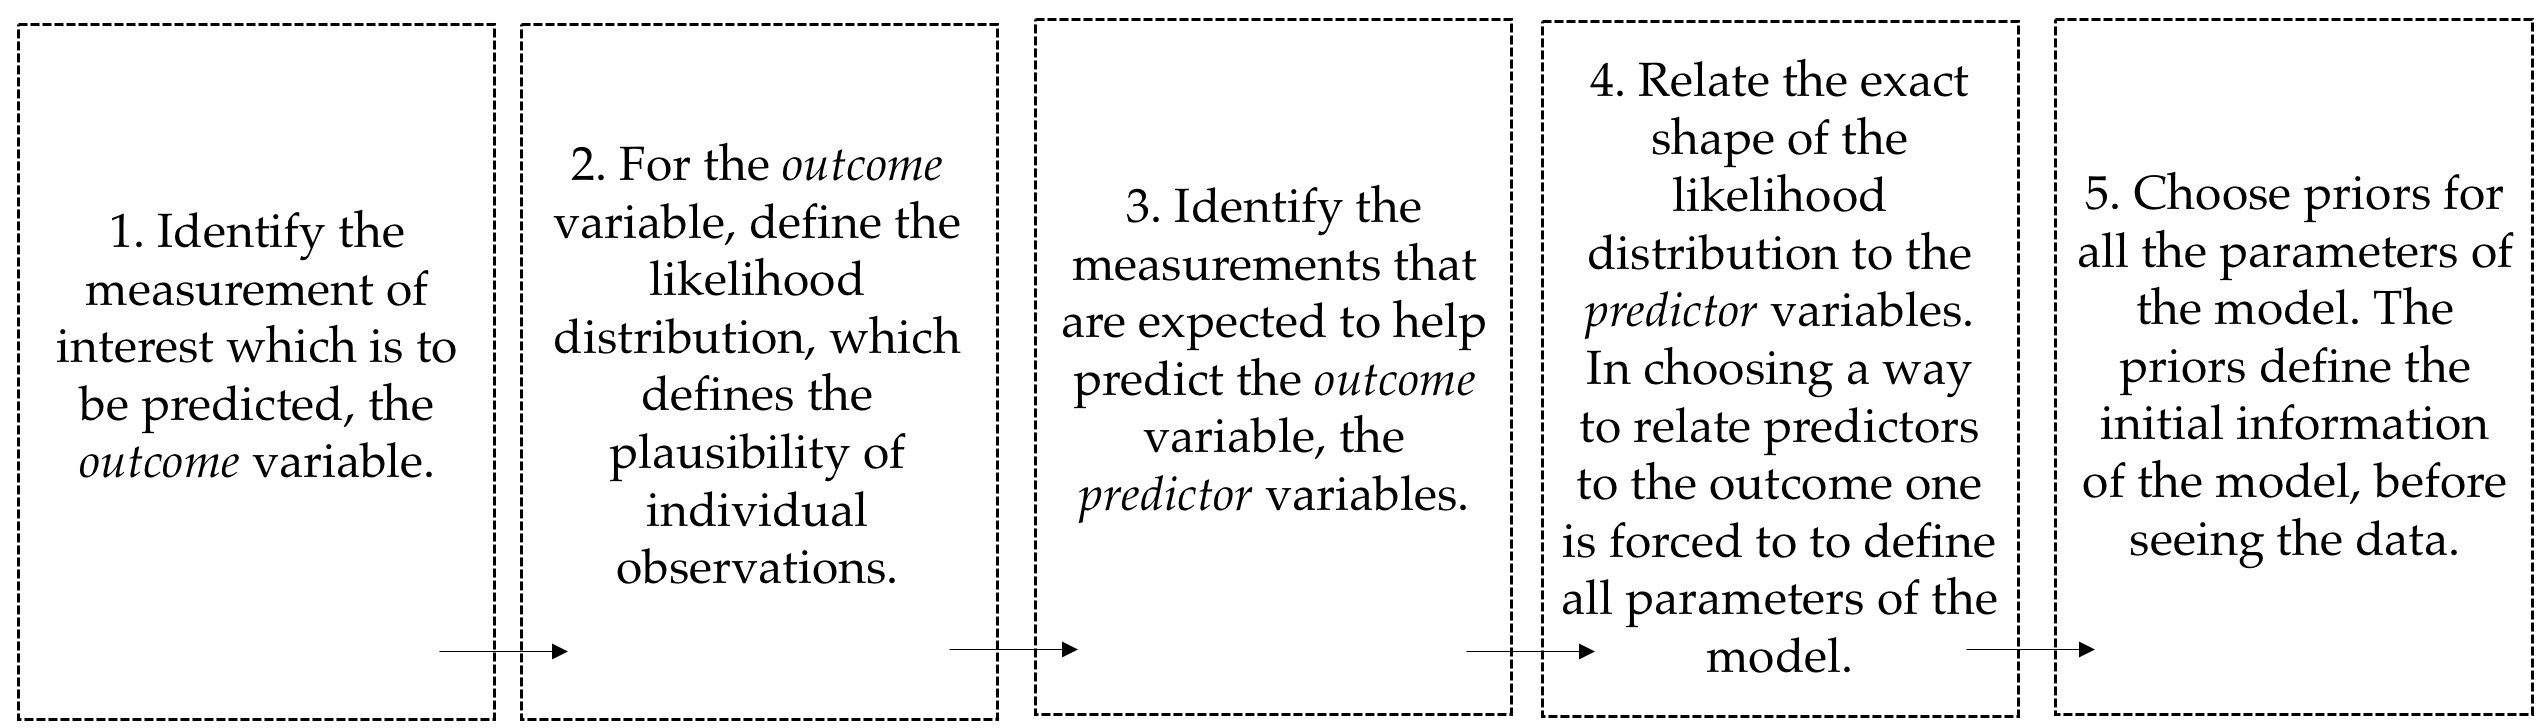
\includegraphics[width=\linewidth]{model_decision_framework}
% \caption{Generic framework to define a model}
% \label{fig:model_decision_framework}
% \caption*{Source: \cite{mcelreath2012}, p.77 [adapted]}
% \end{figure} 

% With these decisions made, the model can be stated, for example, in the format shown in Equation \ref{eq:model}. This format can be retrieved from the example given in Chapter \ref{chp:lit-rev}.

\begin{align}
\label{eq:model}
\text{outcome}_i \sim& Normal(\mu_i, \sigma) && \text{[likelihood]} \\
\mu_i =& \beta \times \text{predictor}_i     && \text{[linear model]}\nonumber\\
\beta \sim& Normal (\mu_\beta, \sigma_\beta) && \text{[prior]}\nonumber\\
\sigma \sim& uniform(a,b) \nonumber          && \text{[prior]}
\end{align}

%  The actual statement for the models are presented in the Appendix \ref{apd:model_statement}.

\subsection{Linear model}

The demand model adopted in this study is the one presented Equation \ref{eq:demand_pdfh}, Chapter \ref{chp:lit-rev}. 

% \begin{equation}
% \label{eq:demand_pdfh}
% V_{i} = a \; \text{GVA}^g_i \; P^f_i \; \text{GJT}^\gamma_i
% \end{equation}
% where

% $V_i$ is volume of journeys, the outcome variable;

% $a$ is a constant;

% $GVA_i$ is the gross added value, one of the predictor variables;

% $P_i$ is the price of the ticket, one of the predictor variables;

% $GJT_i$ is the generalised journey time, one of the predictor variables;

% $g$ is the GVA elasticity of demand;

% $f$ is the price elasticity of demand;

% $\gamma$ is the GJT elasticity of demand.
% \\[3pt]

A stochastic version of this model is given simply by adding the error term into Equation \ref{eq:demand_pdfh}, as shown by Equation \ref{eq:demand_pdfh_stoc}.

\begin{equation}
\label{eq:demand_pdfh_stoc}
V_{i} = a \; {GVA}^g_i \; P^f_i \; GJT^\gamma_i \; e^{u_i}
\end{equation}

A linear alternative to express exponential relationships is the double-log form, as shown by Equation \ref{eq:double_log}. The linear alternative is convenient because it allows estimation by linear regression models and the estimated coefficients can be interpreted as elasticities. %, which allows learning ``about the mean and variance of a measurement using an additive combination of others measures" \citep[p.~71]{mcelreath2012}.

\begin{equation}
\label{eq:double_log}
ln V_{i} = ln \; a + \; g \; ln {GVA}_i + f \; ln P_i + \gamma \; GJT_i + u_i
\end{equation}

Because the interest is to estimate price elasticities of each specific fares, the price component of the model and its elasticity will vary according to the range of available fares in the considered market. Therefore, for Market 1, the price component will be expanded to $f_{2F} ln P_{2F}$ and $f_{2R} ln P_{2R}$, for fares $2F$ and $2R$ respectively. Also, different systems of equations will be estimated for different markets according to the fares available. For instance, in Market 1, there will be two equations: one to estimate the demand of fare 2F and one to estimate the demand of fare 2R. Therefore, the generic form of the equations to be estimated will be, as shown by Equation \ref{eq:generic_model}.

\begin{equation}
\label{eq:generic_model}
ln V_{ki} = ln \; a + \; g \; ln {GVA}_i + \sum{f_{k} \; ln P_{ki}} + \gamma \; GJT_i + u_i
\end{equation}
where

$k$ is the available type of fares in the market.
\\[3pt]

For completeness, the relation of outcomes and predictor variables in each market is shown in the Appendix \ref{apd:linear_models}.

 % It worths highlight that each elasticity regards the demand estimated in its respective equation. Therefore, for market 1, for instance, the first equation will give estimates of fare elasticities $f_{2F}$ and $f_{2R}$ with respect to $V_{2F}$, and the second equation with respect to $V_{2R}$. This was omitted to avoid over subscription in the equations.

% \begin{landscape}
% 
% \begin{table}[!ht] \centering 
%   \caption{Estimated models by market} 
%   \label{tbl:equation_panel} 
% {\renewcommand\arraystretch{1.25}}
% \begin{tabular} {clll}
% \toprule
% Market            & Estimated Equations & Fares Elasticities\\
% \hline
% \multirow{2}{*}{1}&$V_{2Fi} = g{GVA}_i + f_{2F}P_{Fi} + f_{2R}P_{Fi} + \gamma GJT_i $ & $f_{2F}$ and $f_{2R}$, w.r.t. $V_{2F}$\\
%                   &$V_{2Ri} = g{GVA}_i + f_{2F}P_{Fi} + f_{2R}P_{Fi} + \gamma GJT_i $ & $f_{2F}$ and $f_{2R}$, w.r.t. $V_{2R}$\\


% \hline
% \multirow{3}{*}{2}&$V_{2Fi} = g{GVA}_i + f_{2F}P_{2Fi} + f_{2R}P_{Fi} + f_{2A}P_{2Ai} + \gamma GJT_i $ & $f_{2F}$, $f_{2R}$ and $f_{2A}$, w.r.t. $V_{2F}$\\
%                   & $V_{2Ri} = g{GVA}_i + f_{2F}P_{2Fi} + f_{2R}P_{2Ri} + f_{2A}P_{2Ai} + \gamma GJT_i $ & $f_{2F}$, $f_{2R}$ and $f_{2A}$, w.r.t. $V_{2R}$\\
%                   & $V_{2Ai} = g{GVA}_i + f_{2F}P_{2Fi} + f_{2R}P_{2Ri} + f_{2A}P_{2Ai} + \gamma GJT_i $ & $f_{2F}$, $f_{2R}$ and $f_{2A}$, w.r.t. $V_{2A}$\\
 

%  \hline
% \multirow{4}{*}{3}&$V_{1Ni} = g{GVA}_i + f_{1N}P_{1Ni} + f_{2F}P_{2Fi} + f_{2R}P_{2Ri} + f_{2A}P_{2Ai} + \gamma GJT_i $ & $f_{1N}$, $f_{2F}$, $f_{2R}$ and $f_{2A}$, w.r.t. $V_{1N}$\\
%                   &$V_{2Fi} = g{GVA}_i + f_{1N}P_{1Ni} + f_{2F}P_{2Fi} + f_{2R}P_{2Ri} + f_{2A}P_{2Ai} + \gamma GJT_i $ & $f_{1N}$, $f_{2F}$, $f_{2R}$ and $f_{2A}$, w.r.t. $V_{2F}$\\
%                   &$V_{2Ri} = g{GVA}_i + f_{1N}P_{1Ni} + f_{2F}P_{2Fi} + f_{2R}P_{2Ri} + f_{2A}P_{2Ai} + \gamma GJT_i $ & $f_{1N}$, $f_{2F}$, $f_{2R}$ and $f_{2A}$, w.r.t. $V_{2R}$\\
%                   &$V_{2Ai} = g{GVA}_i + f_{1N}P_{1Ni} + f_{2F}P_{2Fi} + f_{2R}P_{2Ri} + f_{2A}P_{2Ai} + \gamma GJT_i $ & $f_{1N}$, $f_{2F}$, $f_{2R}$ and $f_{2A}$, w.r.t. $V_{2A}$\\
 

%  \hline
% \multirow{6}{*}{4}&$V_{1Fi} = g{GVA}_i + f_{1F}P_{1Fi} + f_{1R}P_{1Ri} + f_{1A}P_{1Ai} + f_{2F}P_{2Fi} + f_{2R}P_{2Ri} + f_{2A}P_{2Ai} + \gamma GJT_i $ & $f_{1N}$, $f_{2F}$, $f_{2R}$ and $f_{2A}$, w.r.t. $V_{1F}$\\
%                   &$V_{1Ri} = g{GVA}_i + f_{1F}P_{1Fi} + f_{1R}P_{1Ri} + f_{1A}P_{1Ai} + f_{2F}P_{2Fi} + f_{2R}P_{2Ri} + f_{2A}P_{2Ai} + \gamma GJT_i $ & $f_{1N}$, $f_{2F}$, $f_{2R}$ and $f_{2A}$, w.r.t. $V_{1R}$\\
%                   &$V_{1Ai} = g{GVA}_i + f_{1F}P_{1Fi} + f_{1R}P_{1Ri} + f_{1A}P_{1Ai} + f_{2F}P_{2Fi} + f_{2R}P_{2Ri} + f_{2A}P_{2Ai} + \gamma GJT_i $ & $f_{1N}$, $f_{2F}$, $f_{2R}$ and $f_{2A}$, w.r.t. $V_{1A}$\\
%                   &$V_{2Fi} = g{GVA}_i + f_{1F}P_{1Fi} + f_{1R}P_{1Ri} + f_{1A}P_{1Ai} + f_{2F}P_{2Fi} + f_{2R}P_{2Ri} + f_{2A}P_{2Ai} + \gamma GJT_i $ & $f_{1N}$, $f_{2F}$, $f_{2R}$ and $f_{2A}$, w.r.t. $V_{2F}$\\
%                   &$V_{2Ri} = g{GVA}_i + f_{1F}P_{1Fi} + f_{1R}P_{1Ri} + f_{1A}P_{1Ai} + f_{2F}P_{2Fi} + f_{2R}P_{2Ri} + f_{2A}P_{2Ai} + \gamma GJT_i $ & $f_{1N}$, $f_{2F}$, $f_{2R}$ and $f_{2A}$, w.r.t. $V_{2R}$\\
%                   &$V_{2Ai} = g{GVA}_i + f_{1F}P_{1Fi} + f_{1R}P_{1Ri} + f_{1A}P_{1Ai} + f_{2F}P_{2Fi} + f_{2R}P_{2Ri} + f_{2A}P_{2Ai} + \gamma GJT_i $ & $f_{1N}$, $f_{2F}$, $f_{2R}$ and $f_{2A}$, w.r.t. $V_{2A}$\\
% \bottomrule\end{tabular}%
% \caption*{Source: own elaboration}
% \end{table} 


\begin{table} \centering 
  \caption{Linear models by market} 
  \label{tbl:equation_panel} 
{\renewcommand\arraystretch{1.25}}
\begin{tabular} {cl}
\toprule
Market            & Equations \\
\hline
\multirow{2}{*}{1}&$lnV_{2Fi} = ln \; a + g \; ln{GVA}_i + f_{2F} \; lnP_{2Fi} + f_{2R} \; lnP_{2Ri} + \gamma \; lnGJT_i$ \\
                  &$lnV_{2Ri} = ln \; a + g \; ln{GVA}_i + f_{2F} \; lnP_{2Fi} + f_{2R} \; lnP_{2Ri} + \gamma \; lnGJT_i$ \\


\hline
\multirow{3}{*}{2}&$lnV_{2Fi} = ln \; a + g \; ln{GVA}_i + f_{2F} \; lnP_{2Fi} + f_{2R} \; lnP_{2Ri} + f_{2A} \; lnP_{2Ai} + \gamma \; lnGJT_i$\\
                  &$lnV_{2Ri} = ln \; a + g \; ln{GVA}_i + f_{2F} \; lnP_{2Fi} + f_{2R} \; lnP_{2Ri} + f_{2A} \; lnP_{2Ai} + \gamma \; lnGJT_i$\\
                  &$lnV_{2Ai} = ln \; a + g \; ln{GVA}_i + f_{2F} \; lnP_{2Fi} + f_{2R} \; lnP_{2Ri} + f_{2A} \; lnP_{2Ai} + \gamma \; lnGJT_i$\\
 

 \hline
\multirow{4}{*}{3}&$lnV_{1Ni} = ln \; a + g \; ln{GVA}_i + f_{1N} \; lnP_{1Ni} + f_{2F} \; lnP_{2Fi} + f_{2R} \; lnP_{2Ri} + f_{2A} \; lnP_{2Ai} + \gamma \; lnGJT_i$\\
                  &$lnV_{2Fi} = ln \; a + g \; ln{GVA}_i + f_{1N} \; lnP_{1Ni} + f_{2F} \; lnP_{2Fi} + f_{2R} \; lnP_{2Ri} + f_{2A} \; lnP_{2Ai} + \gamma \; lnGJT_i$\\
                  &$lnV_{2Ri} = ln \; a + g \; ln{GVA}_i + f_{1N} \; lnP_{1Ni} + f_{2F} \; lnP_{2Fi} + f_{2R} \; lnP_{2Ri} + f_{2A} \; lnP_{2Ai} + \gamma \; lnGJT_i$\\
                  &$lnV_{2Ai} = ln \; a + g \; ln{GVA}_i + f_{1N} \; lnP_{1Ni} + f_{2F} \; lnP_{2Fi} + f_{2R} \; lnP_{2Ri} + f_{2A} \; lnP_{2Ai} + \gamma \; lnGJT_i$\\ 
 \hline
\multirow{6}{*}{4}&$lnV_{1Fi} = ln \; a + g \; ln{GVA}_i + f_{1F} \; lnP_{1Fi} + f_{1R} \; lnP_{1Ri} + f_{1A} \; lnP_{1Ai} + f_{2F} \; lnP_{2Fi} + f_{2R} \; lnP_{2Ri} + f_{2A} \; lnP_{2Ai} + \gamma \; lnGJT_i$\\
				  &$lnV_{1Ri} = ln \; a + g \; ln{GVA}_i + f_{1F} \; lnP_{1Fi} + f_{1R} \; lnP_{1Ri} + f_{1A} \; lnP_{1Ai} + f_{2F} \; lnP_{2Fi} + f_{2R} \; lnP_{2Ri} + f_{2A} \; lnP_{2Ai} + \gamma \; lnGJT_i$\\
				  &$lnV_{1Ai} = ln \; a + g \; ln{GVA}_i + f_{1F} \; lnP_{1Fi} + f_{1R} \; lnP_{1Ri} + f_{1A} \; lnP_{1Ai} + f_{2F} \; lnP_{2Fi} + f_{2R} \; lnP_{2Ri} + f_{2A} \; lnP_{2Ai} + \gamma \; lnGJT_i$\\
				  &$lnV_{2Fi} = ln \; a + g \; ln{GVA}_i + f_{1F} \; lnP_{1Fi} + f_{1R} \; lnP_{1Ri} + f_{1A} \; lnP_{1Ai} + f_{2F} \; lnP_{2Fi} + f_{2R} \; lnP_{2Ri} + f_{2A} \; lnP_{2Ai} + \gamma \; lnGJT_i$\\
				  &$lnV_{2Ri} = ln \; a + g \; ln{GVA}_i + f_{1F} \; lnP_{1Fi} + f_{1R} \; lnP_{1Ri} + f_{1A} \; lnP_{1Ai} + f_{2F} \; lnP_{2Fi} + f_{2R} \; lnP_{2Ri} + f_{2A} \; lnP_{2Ai} + \gamma \; lnGJT_i$\\
				  &$lnV_{2Ai} = ln \; a + g \; ln{GVA}_i + f_{1F} \; lnP_{1Fi} + f_{1R} \; lnP_{1Ri} + f_{1A} \; lnP_{1Ai} + f_{2F} \; lnP_{2Fi} + f_{2R} \; lnP_{2Ri} + f_{2A} \; lnP_{2Ai} + \gamma \; lnGJT_i$\\

\bottomrule\end{tabular}%
\caption*{Source: Own work}
\end{table} 

% \end{landscape}

\subsection{Likelihood}
% 300 words

The first thing to consider to define the likelihood is the scale type of the outcome variable - whether metric, ordinal, nominal or count. Because things can be measured in different scales, different probability measure may apply and ``the likelihood function must specify a probability distribution on the appropriate scale" \citep[p.~423]{kruschke2014}.

For this study, the outcome variable - \textit{journeys} - can be considered as metric scale, since its value actually provides a quantity of what is being measured - even though it is transformed to logarithmic form. 

For this kind of scale, the most usual probability distribution is the normal. \cite{mcelreath2012} discuss two main reasons that can justify it.

The first one regards the fact the normal distribution has the property to represent phenomenons that are sum of fluctuations of other phenomenons, irrespective of their original distribution. ``Repeatedly adding finite fluctuations results in a distribution of sums that shed all information about the underlying process, aside from mean and spread" \citep[p.~75]{mcelreath2012}. In this sense, it might be plausible to interpret the number of rail journeys as a resultant phenomenon of fluctuations of the subprocess. People often make travel decision based on a general range of factors, and the way they usually vary in time and region may represent the fluctuations mentioned.

The second reason regards the fact that the normal distribution ``represents a particular state of ignorance" \citep[p.~75]{mcelreath2012}. This represents the most convenient form to express the lack of knowledge about a variable because its shape can comprise several different assumptions.

This also seems to be applicable to our variable. Putting in another way, one may not have evidence that this should not assume a normal distribution and this ignorance may suggest normal it is appropriate.

Therefore, the likelihood which will be applied for all models will be such as $ln V_i \sim Normal(\mu_i, \sigma)$.

\subsection{Priors} 

When defining a prior distribution, one must be aware of two aspects of it: first it regards the definition of an interval for credible values that the parameter can assume; second, regards the shape of the probability density in this interval. To consider these elements for the current case, one may first recover the parameters presented in Equation \ref{eq:demand_pdfh}, summarised by Table \ref{tbl:param_priors}.


\begin{table}[!ht] \centering 
  \caption{Model's parameters that demand prior distributions} 
  \label{tbl:param_priors} 
{\renewcommand\arraystretch{1.25}}
\begin{tabular} {clc}
\toprule
\multirow{2}{*}{Parameter}  & \multirow{2}{*}{Measure}  & Expected \\
                            &                           & Sign \\
\hline
\multirow{2}{*}{$f$}        & price elasticity of demand.& own: negative \\
		   & It can regard the own or cross elasticity.  & cross: positive\\
$g$        & GVA elasticity of demand. & positive \\ 
$\gamma$   & GJT elasticity of demand. & negative\\
$\sigma$   & standard deviation of the outcome variable.& N.A.\\
\bottomrule
\end{tabular}%
\caption*{Source: Own work}
\end{table} 



Starting for the price elasticity, it will be convenient divide it in two discussions: the own elasticity prior and the cross elasticity prior. This is relevant because of the assumption adopted from the PDFH that the differently available fares are competitors, thus the cross elasticity should expect to be positive, and the own elasticity should expect to be negative. 

Recovering that the price elasticity measures how much the demand responds to a change in price, in percentage terms, one may consider plausible that credible values for the own price elasticities of demand in this study should be somewhere between zero and -1. This interval covers circumstances which go from a complete inelastic demand, which does not vary irrespective of a change in price, to an elastic demand, in which case a change in price causes a proportional change in the demand in the opposite direction. It eventually could be lower than -1, for a very price-sensitive demand, but it would not be reasonable considering that there is no lower boundary, even though setting one may be arbitrary.

For the cross elasticity, the rationale is analogous but the values are symmetric, so a credible interval would be between zero and 1. Again, it would eventually be greater than 1, even though it may be arbitrary setting an upper boundary. 

% IS IT POSSIBLE TO DISCUSS THAT THE CROSS ELASTICITIES ARE SMALLER THAN THE OWN ELASTICITIES?
% To complement this analysis, it should be also considered that cross-elasticities should be expected to be smaller that the own elasticities of demand. Cross-elasticity, opposed to the own-elasticity, regards a marginal effect of a change in the price of a secondary good. For instance, when a price of good B increases, its own demand may be reduced because consumers stop to consume it or because they migrate to competitive  it may reflect the demand of 

In what regards the shape of the probability density across the credible values for price elasticities, economic theory provides no evidence abaout it, which may lead to the adoption of a uniform probability. However, the guidances from the statistical package used in this work - Stan \citep{stan}, suggests as a general principle that uniform priors should not be applied ``unless the boundaries represent true constraints" \citep{stan_prior}. Despite one of the boundaries actually represent a constraint - the upper boundary is zero for own elasticity and the lower boundary is also to zero for the cross elasticity - the others boundaries would be defined arbitrarily. Therefore, adopting uniform distribution would be not a goodd practice. 

The suggested solution is to stablish a normal distribution centred in the credible interval. Indeed, there are specific guidances for elasticities estimates in double-log regressions that recommends that normal distribution with mean $0.5$ and standard deviation of $0.5$ is a good default prior.

To ensure that the theoretical constraints will be respected, a one-sided restriction will be applied, as pertinent. As introduced in Chapter \ref{chp:lit-rev}, the possibility of applying constraints is one of the advantages of Bayesian inference. 

For own price elasticities, the prior will be defined as $f \sim Normal(-0.5, 0.5)$, truncated at zero at the upper boundary ($T[ \quad , 0]$); and for cross price elasticities, $f_x \sim Normal(0.5, 0.5)$, trucated at zero at the lower bound ($T[0, \quad]$).

For the GVA elasticity of demand, the prior knowledge suggests a positive polarity between the rail demand and the GVA, as already discussed in the exploratory analysis of the data in this Chapter. Even though the GVA elasticity is expected to be positive, this single piece of information is not enough to define the interval for credible values and the shape of probability density function. It will be convenient, thus, follow the guidances from the statistical package - Stan. A suggested generic prior is recommended to be Normal(0,1). The guidance highlights that this prior may limit extreme values because the normal distribution has shorter tails than other bell-shaped distributions. 

The GJT elasticity of demand is analogous to the GVA but in the opposite direction. As discussed in the exploratory analysis, an increase in GJT tends to cause decrease in the demand, so a negative coefficient should be expected. For the same reasons presented for the GVA elasticity, it will also be adopted the generic prior Normal(0,1) to the GJT parameter.

Lastly, as done for the price elasticity priors, to ensure right algebraic signs, the prior distribution for GVA and GJT elasticities will be constrained by a lower and upper boundary at zero, respectively. 

% Lastly, despite being possible to restrict the values to be positive or negative for both GVA and GJT parameters, as was done in the price elasticity priors, it would not be done to avoid unnecessary constraints in the model. Unless it became necessary to correct the algebraic sign of the estimate, they will not be restricted.

Therefore, for the GVA and the GJT's elasticities the prior applied will be $g \sim Normal(0,1)$, truncated at zero at the lower boundary ($T[0, \quad ]$) and $\gamma \sim Normal(0,1)$, truncated at zero at the upper boundary ($T[ \quad , 0]$), respectively. 

For the $\sigma$ prior there is no evident definition for a range of credible values, despite the fact that it is by nature a positive value. It was adopted the default distribution from Stan - uniform prior on ($-\infty$, $\infty$) \citep{stan-manual} - constrained by the positive domain. Therefore, the resulting $\sigma$'s prior was $\sigma \sim uniform(0,\infty)$.

% The whole model is presented in the Appendix \ref{apd:model_statement}. 

% \textit{Prior Sensitivness}

\section{Calibration and target measures}

As mentioned, the Bayesian models were estimated with the aid of the \textit{Stan}, a software package. In this package the posterior distributions are approximated using a Markov Chain of Monte Carlo called \textit{Hamiltonia Monte Carlo}, a variation of the Metropolis algorithm.

Some elements of the estimation process that are important to interpret the results regard the calibration of the process in terms of number of iterations, warm-up period, thinness, number of chains, initial values, effective sample and autocorrelation measures, and convergence. A brief definition and the default adopted in this work are presented in the following.

The quantity of iterations regards the length of the Markov Chain that will be run to build the posterior distribution. The longer it is, the more defined the posterior gets. However, it does not mean that one needs to exhaust computation resources to get a reasonable draw of posterior distributions. For this work, the standard number of iterations adopted was $2,000$. It is supposed to be enough to achieve convergence without autocorrelated samples, for non-complex models. Eventually, more iterations may be demanded.

Still regarding the number of iterations, is the warm-up period, which is ``the practice of discarding early iterations in Markov Chain (...) to diminish the influence of starting values" \citep{gelman2014}. The discarded ratio may vary according to the circumstances, but for a conservative approach, it will be adopted to discard the first half of the iterations. Therefore, running $2,000$ iterations, the first $1,000$ will be discarded.

Another aspect of the Markov Chain regards thinness of steps, which is the rule of which steps are kept as a draw for the posterior. It is usually defined as 1, so each iteration is kept. Nevertheless, it may be increased to reduce autocorrelation \citep{kruschke2011} - instead of keeping each iteration, one keeps only every $n^{th}$ step. An implication of increasing the thinness of an estimation is that it reduces the iterations kept, which might demand as a counterpart the increase of the number of iterations proportionally. In this study it will be adopted thin = 1. If it eventually demands to be increased to $n$, the interactions will be $2,000 \cdot n$.

Despite defining the number of iterations and its related attributes, it is also necessary to define the number of chains. After the warm-up period the variance within the chain is supposed to be stable, so one may consider that it has achieved convergence. However, for a reliable inference, it is also important to check whether different independent sequences will converge to the same distribution. In this study, it will be adopted the default of 3 chains. When discussing the results a measure for convergence will be the $\hat{R}$, the potential scale reduction factor. When convergence is achieved, $\hat{R}=1$.

Another element that needs to be calibrated in the estimation procedure is the initial values from which the Markov Chains will start. For this study the default will not be explicitly defined. Instead, they will be randomly generated by the software \citep{stan-manual}.

Lastly, there is the the effective sample size ($n_{\text{eff}}$), which is not an element to be calibrated in the process but an output used to judge the quality of the resulting posterior distribution in combination with the $\hat{R}$. As long it will be used in Chapter \ref{chp:results}, it worths introducing its concept. 

When samples are autocorrelated in the chain the estimation might become inefficient because it does not fully explore the probability space of the parameters, instead it may get stuck. The $n_{\text{eff}}$ is a measure that discount autocorrelated samples, providing a sense of the number of independent samples drawn to estimate the posterior distribution. As a default rule, \cite{gelman2014} suggests running the simulation until $n_{eff}$ is at least ten times the number of chains. Therefore, since the estimation will run with 3 chains, the $n_{\text{eff}}$ must be higher than 30.
\chapter{Results}
\label{chp:results}

\section{General guidances on interpretation of the results}

To interpret the results one must keep in mind that the estimated coefficients are elasticities. The practical implication of this is that the coefficient values represent the percentual change in the demand for a one percent change in the variable (untransformed to log). Therefore, a coefficient of value $1$ will mean a one percent change in the demand for a one percent change in the predictor variable - fares, GVA or GJT. 

% Another way of stating that is that a coefficient whose value is 1 means that the demand changes proportionally to the change in the predictor variables. When the coefficient is higher than 1 the impact in the demand is more than proportional and, conversely, when it is less, the impact is lower than proportional. Additionally, the proportion of variation above or below the proportional change can, in turn, be stated as a percentage. Thus, for instance, a coefficient whose values is $1.2$ means that the impact in the demand is 20\% more than proportional, and for a coefficient $0.8$, this impact would be 20\% less than proportional.

% Comment on elastic and inelastic

Beyond the point estimates, the Bayesian regression provides a probability density function (pdf) of credible values that the coefficients may assume. In fact, the point estimate is the mean of the posterior distribution. 

An advantage of a pdf output over a point estimate is that it is possible to directly interpret the probabilities of values in a given interval. For instance, one can take two values and compute the probability of the coefficient being in the interval. This is fundamentally different from the frequentist confidence interval, which only regards the probability of a sampling procedure resulting in an interval which contains the true value of the estimated parameter.

The posterior distributions are convenient to discuss the uncertainty of estimates. The usual procedure is taking the high-density interval (HDI) to consider the boundaries of credible values for the coefficients. The HDI is the smallest interval to achieve a given probability, which may differs from the symmetrical density interval, as illustrated by Figure \ref{fig:hdi}, when the distribution is not symmetrical. 

In this work, a HDI of 95\% will be adopted in the analysis. Full information on the estimated HDI is presented on Appendix \ref{apd:bayes_hdi} .

The analysis of the results will be presented with the aid of marginal posterior distribution's plots. This format is useful since it is a bi-dimensional figure, but it worths recovering that the actual posterior distribution, as discussed in Chapter \ref{chp:lit-rev} is a multi-dimensional space, where the dimensions depend on the number of predictor variables.

\begin{figure}
\centering
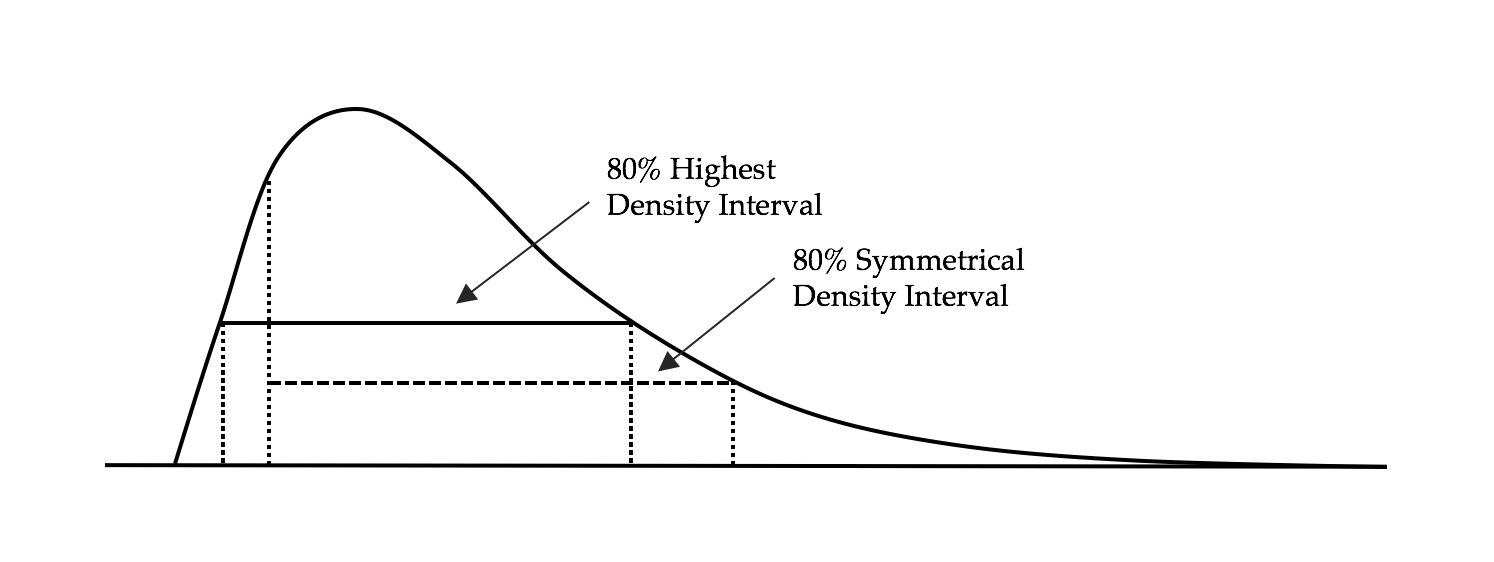
\includegraphics[scale=0.4]{hdi}
\caption{High Density Interval \textit{versus} Symmetrical Density Interval}
\label{fig:hdi}
\caption*{Source: \cite{hdinterval} [adapted]}
\end{figure}

% The advantage of the posterior distribution is that they can be directly interpreted as probabilities in a given interval, which will be useful to discuss the uncertainty around the point estimate. For instance, one can discuss the amplitude of an interval regarding the difference between the lowest and highest values within an HDI. The practical application of analysing the amplitude is measuring how much uncertainty there is between these extreme probable values. Consider, for instance, an elasticity density function whose HDI 95\% is between 1.2 and 1.3. This would mean that the lower probable value of elasticity would be 1.2, which in turn means that demand would vary 20\% for a given percentage change in the predictor, say fare. The highest probable value would be 1.3, which in turn means that demand would vary 30\% for a given percentage change in the same predictor. The conclusion is that there is a small range of values that makes the uncertainty around the elasticity's coefficient varies only 10\%.

An additional consideration when interpreting the posterior distribution plots is that the y axis would eventually be greater than one. This is apparently counter-intuitive since probabilities are defined in the [0,1] domain. However, because it is a continuous function, the actual probability of the estimate assuming a point value is zero. So the y axis should be not be used to directly read the probabilities from values in the x axis. Instead, a probability can only be computed integrating a given an interval. Integrating the full density function it would be approximately 1 \citep{kruschke2014}.

\section{Comparative Estimates: SURE/OLS Models}

For a comparison purpose, frequentist estimates will be provided along the Bayesian estimates. The most plausible approach would be the seemingly unrelated regression estimation (SURE), nevertheless, despite it seems natural to think about the demand estimation for each market as a system of demand equations (one for each type of fare), as taught by \cite{kennedy2003}, SURE estimation becomes identical to OLS when all the predictive variables are the same, which happens to be the case in this study.

The models were estimated based on the linear models presented in Table \ref{tbl:equation_panel}. As it should be expected, the estimation of SURE/OLS models reinforces previous studies showing that ``freely estimating models will not yield robust elasticities" \citep[p.~37]{its-systra-report}. Despite statistically significant - with some exceptions - several estimated elasticities presented unexpected signs, according to the assumptions of the PDFH. Table \ref{tbl:summary_ols} summarises the occurrences. 


\begin{table}[H] \centering 
  \caption{Summary of SURE/OLS outputs with respect to algebraic sign of coefficients} 
  \label{tbl:summary_ols} 
{\renewcommand\arraystretch{1.25}}
\begin{tabular} {cccccc}
\toprule
\multirow{2}{*}{Market} & Dependent & \multicolumn{4}{c}{Elasticities Estimates} \\
\cline{3-6} 
                        & Variable  & \multicolumn{2}{c}{Expected Sign} & \multicolumn{2}{c}{Unexpected Sign} \\
\hline
\multirow{2}{*}{1}      &$ln V_{2F}$& 4 & $f_{2F}$, $f_{2R}$, $g$, $\gamma$                                           & - & - \\
\cdashline{2-6} 
						&$ln V_{2R}$& 3 & $f_{2F}$, $f_{2R}$, $\gamma$                                                & 1 & $g$ \\
\hline
\multirow{3}{*}{2}      &$ln V_{2F}$& 4 & $f_{2F}$, $f_{2A}$, $g$, $\gamma$                                           & 1 & $f_{2R}$ \\
\cdashline{2-6} 
						&$ln V_{2R}$& 4 & $f_{2F}$, $f_{2R}$, $g$, $\gamma$                                           & 1 & $f_{2A}$  \\
\cdashline{2-6} 
						&$ln V_{2A}$& 3 & $f_{2R}$, $f_{2A}$, $g$                                                     & 2 & $f_{2F}$, $\gamma$ \\
\hline
\multirow{4}{*}{3}      &$ln V_{1N}$& 6 & $f_{1N}$, $f_{2F}$, $f_{2R}$, $f_{2A}$, $g$, $\gamma$                       & - & - \\
\cdashline{2-6} 
						&$ln V_{2F}$& 4 & $f_{2F}$, $f_{2A}$, $g$, $\gamma$                                           & 2 & $f_{1N}$, $f_{2R}$ \\
\cdashline{2-6} 
						&$ln V_{2R}$& 4 & $f_{2F}$, $f_{2A}$, $g$, $\gamma$                                           & 2 & $f_{1N}$, $f_{2R}$ \\
\cdashline{2-6} 
						&$ln V_{2A}$& 5 & $f_{2F}$, $f_{2R}$, $f_{2A}$, $g$, $\gamma$                                 & 1 & $f_{1N}$ \\
\hline
\multirow{6}{*}{4}      &$ln V_{1F}$& 8 & $f_{1F}$, $f_{1R}$, $f_{1A}$, $f_{2F}$, $f_{2R}$, $f_{2A}$, $g$, $\gamma$   & - & - \\
\cdashline{2-6} 
						&$ln V_{1R}$& 6 & $f_{1R}$, $f_{2F}$, $f_{2R}$, $f_{2A}$, $g$, $\gamma$                       & 2 & $f_{1F}$, $f_{1A}$ \\
\cdashline{2-6} 
						&$ln V_{1A}$& 6 & $f_{1F}$, $f_{2F}$, $f_{2R}$, $f_{2A}$, $g$, $\gamma$                       & 2 & $f_{1R}$, $f_{1A}$ \\
\cdashline{2-6} 
						&$ln V_{2F}$& 3 & $f_{2A}$, $g$, $\gamma$                                                     & 5 & $f_{1F}$, $f_{1R}$, $f_{1A}$, $f_{2F}$, $f_{2R}$    \\
\cdashline{2-6} 
						&$ln V_{2R}$& 8 & $f_{1F}$, $f_{1R}$, $f_{1A}$, $f_{2F}$, $f_{2R}$, $f_{2A}$, $g$, $\gamma$   & - & - \\
\cdashline{2-6} 
						&$ln V_{2A}$& 7 & $f_{1F}$, $f_{1A}$, $f_{2F}$, $f_{2R}$, $f_{2A}$, $g$, $\gamma$             & 1 & $f_{1R}$ \\
\bottomrule
\end{tabular}%
\caption*{Source: Own work}
\end{table} 

% \textit{GVA}      &\multicolumn{2}{m{6cm}}{\raggedright regional GVA, at NUTS 3 level, in millions of pounds, 2014 values.} 

\section{Bayesian models with weakly informative priors}

Because it is safer to estimate Bayesian models gradually building in complexity, Bayesian models with weakly informative priors were estimated before the constrained models. The priors established for these models have followed the same guidances from Chapter \ref{chp:methods}, but without the truncation.

The models were run without any issues. However, this estimation was of little help in generating estimates with correct algebraic signs resulting in estimates very similar to the OLS. This may be explained due to the high volume of data that makes the likelihood prevails over the prior distribution \citep{kruschke2014}. Therefore, the valuable prior information added to the models was the restriction applied in the domain of the elasticities' probability densities, as discussed in the next section.

For completeness, the Appendix \ref{apd:bayes_weakpriors} presents the results of estimated models with weakly informative priors. 

\section{Bayesian constrained models}

\subsection{Market 1}

\textit{i. Autocorrelation and convergence}

The first market, with only two fares competing, is the simpler one. The model converged with low autocorrelation in the posterior samples, as shown by the statistics in Table \ref{mkt1_T_autocorr_convergence}.

% latex table generated in R 3.3.2 by xtable 1.8-2 package
% Sat Aug  5 10:10:51 2017
\begin{table}[ht]
\caption{Autocorrelation and convergence measures - Market 1}
\label{mkt1_T_autocorr_convergence}
\centering
\begin{tabular}{lrrrrr}
\toprule 
 & \multicolumn{5}{c}{\textit{Dependent variable:}} \\ 
\cline{2-6} 
\\[-1.8ex] & \multicolumn{2}{c}{$ln \; V_{2F}$} & & \multicolumn{2}{c}{ $ln \; V_{2R}$}\\ 
\cline{2-3} \cline{5-6}
 & $\hat{R}$ & $n_{\text{eff}}$ & &$\hat{R}$ & $n_{\text{eff}}$ \\ 
  \midrule

  $f_{2F}$ & 1.0 & 1650 & & 1.0 & 402 \\ 
  $f_{2R}$ & 1.0 & 1692 & & 1.0 & 821 \\ 
  $g$      & 1.0 & 1561 & & 1.0 & 719 \\ 
  $\gamma$ & 1.0 & 1778 & & 1.0 & 432 \\ 
  Constant & 1.0 & 1477 & & 1.0 & 702 \\ 
   \hline
   Iter    & \multicolumn{2}{c}{2,000} && \multicolumn{2}{c}{2,000} \\
   Thin    & \multicolumn{2}{c}{1} && \multicolumn{2}{c}{1} \\
   \bottomrule
\end{tabular}
\caption*{Source: Own work}
\end{table}

It is relevant, however, to consider that a warning of divergent transitions after the warm-up was reported for both regressions. The issue around it is that these warnings signalise that the estimates might be biased \citep{stan_warnings}, even though they have converged to stable and equivalent variances across the chains.

The divergent transitions are likely to be related to the imposition of constraints in the domain of the probability density. This might have prevented the MCMC to explores the parameter space with plausible values according to the likelihood, but constrained by the prior. Therefore, it appears that the divergent transitions are part of the adopted solution of applying restrictions to prevent unfeasible estimates.

It will be assumed, therefore, that biased estimates are the best information at hand and should not be discarded. As taught by \cite{gelman_blog}, in the context of Bayesian data analysis, one should recognise that ``unbiasedness" is a very idealistic concept, and because it may hardly be achieved, one should not refrain oneself to make usage of the available information.
\\[3pt]

\textit{ii. OLS comparison}

A comparison between the Bayes and OLS estimates is presented in Table \ref{tbl:mkt1_T}. As expected, the all Bayesian coefficients have coherent signs. It has clearly improved the estimation of $g$ with respect to the $V_{2R}$ demand, for which the OLS estimation has failed.

% In general terms, it is possible to say that no big discrepancies were observed from the two estimates and their respective standard deviations, excepted for the $g$ parameter. This is easier to see with the aid of the Figures ahead.

% latex table generated in R 3.3.2 by xtable 1.8-2 package
% Mon Jul 31 09:29:49 2017
\begin{table} [H]
\caption{Comparison of bayesian and SURE/OLS estimates - Martket 1}
\label{tbl:mkt1_T}
\centering
\begin{tabular}{rrrrrrrrrrr}
  \toprule 
 & \multicolumn{2}{c}{\textit{Bayes}} & & \multicolumn{2}{c}{\textit{SURE/OLS}} \\ 
\cline{2-3} \cline{5-6}
\\[-1.8ex] & $ln \; V_{2F}$ & $ln \; V_{2R}$ & & $ln \; V_{2F}$ & $ln \; V_{2R}$ \\ 
\hline \\[-1.8ex] 

  $f_{2F}$ & -1.32 & 0.70 & &-1.28 & 0.81\\
  		   & (0.05)  & (0.05) & & (0.05) & (0.05)\\ [0.2cm]
  $f_{2R}$ & 0.17 & -0.89  & & 0.17 & -0.89 \\
  			& (0.05) &  (0.05) & & (0.05) & (0.05)\\ [0.2cm]
  $g$ & 0.77 & 0.06 & & 0.49 & \cellcolor{gray!25}-0.52 \\
  		& (0.05) & (0.04) & & (0.7) & (0.7)\\ [0.2cm]
  $\gamma$ & -0.89 & -0.88 & & -0.98 & -1.06\\
  			& (0.04) & (0.05) & & (0.04) & (0.05)\\ [0.2cm]
  Constant & 6.10 & 11.27 & & 9.14 & 17.6\\
  			& (0.57) & (0.47) & & (0.71) & (0.73)\\ [0.2cm]
  % \hline
  % $\sigma$ & 1.43 & 1.48 & & -& -\\
  % 		 & (0.01) & (0.01) & & -& -\\
\bottomrule
\end{tabular}
\caption*{Source: Own work}
\end{table}


\textit{iii. Uncertainty}

% 1.
Figures \ref{fig:mkt1_v2f_post} and \ref{fig:mkt1_v2r_post} present the marginal posterior distribution of the estimated elasticities coefficients. The continuous lines represent the Bayesian mean, the red line represents the OLS mean and the dotted lines represent the boundaries of the 95\% HDI.

% 2.
As one may notice, the small standard deviations are reflected in a posterior distribution with a decimal scale for all estimates, except the constant - which usually will not be covered in the analysis. These small ranges of credible values for the coefficients are useful since these are elasticities measures. It is important that they do not allow the distribution to spread much, becoming low-quality information. 

This is also reflected in the HDI boundaries, which are very close to the mean value demonstrating that there is a small range of credible values. As a general rule, it will be considered that an HDI up 0.30 is satisfactorily small. Above this value, the uncertainty would be unfavourable to any practical application since this decimal variation in the coefficient, in fact, is a percent impact on the demand. Detailed information of the HDI is presented in the Appendix \ref{apd:bayes_hdi}. 

% 3ab.
With respect to the $V_{2f}$ demand, Figure \ref{fig:mkt1_v2f_post}, all elasticities distributions are smooth bell-shaped curves, demonstrating that they have not faced any strong constraint. Indeed, the OLS estimate already had the correct signs, so there was no conflict in the estimation.

% 3c.
Even though the OLS estimates had correct signs, some of them were not considered credible values according to the Bayesian estimation: the $g$ elasticity lied out of the HDI and the $\gamma$ was at the edge. 

\begin{figure}[H]
\centering
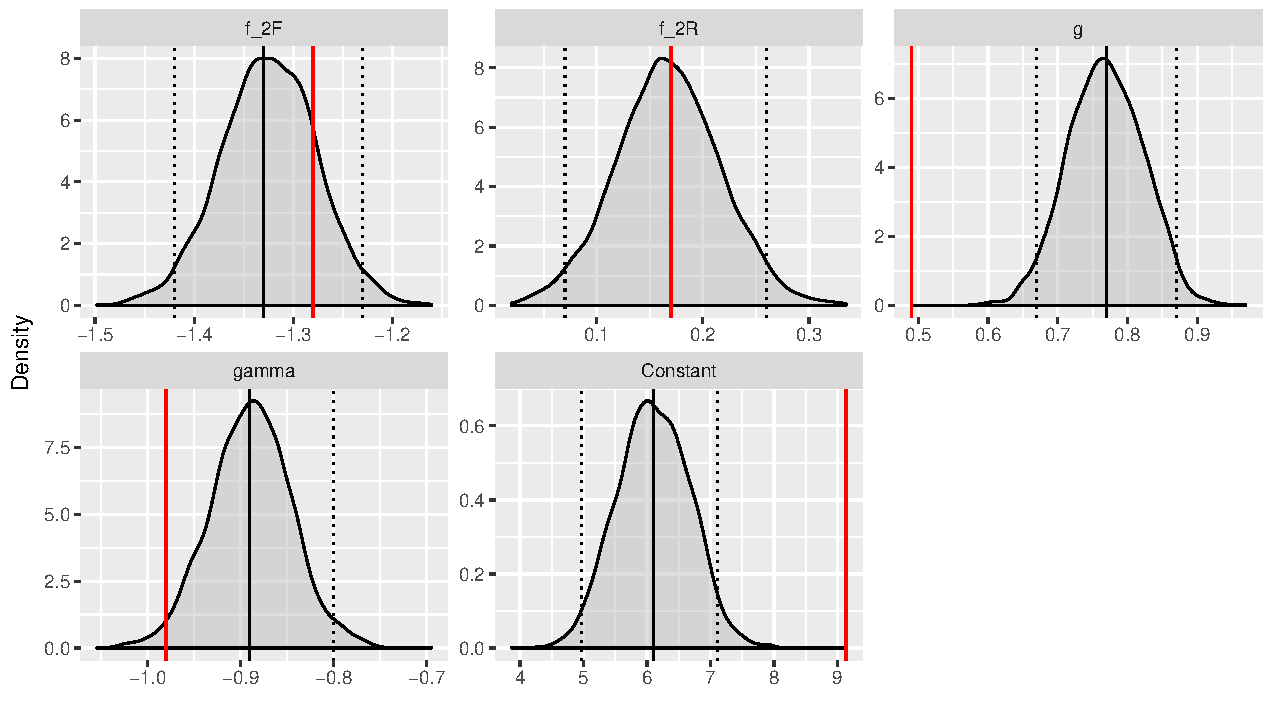
\includegraphics[width=\linewidth]{mkt1_v2f_post.pdf}
\caption{Posterior density function of elasticities w.r.t $V_{2F}$ - Market 1}
\label{fig:mkt1_v2f_post}
\caption*{Source: Own work}
\end{figure} 

% 3a.
With respect to the $V_{2R}$ demand, Figure \ref{fig:mkt1_v2r_post}, the curves are bell-shaped, except for the $g$ which is skewed towards the left. It is noticeable that this is the sign-reverted elasticity. It appears that the constraint at zero, which blocked the distribution to assume negative values, was an actual barrier. Indeed this may explain the warnings of divergent transitions.

% 3b.
All HDI were satisfactorily small, from 0.14 to 0.20. 

% 3c.
The OLS estimates of $f_{2F}$, $g$ and $\gamma$ are out of the HDI, demonstrating that these are not credible values according to the Bayesian estimation. Opposedly, the OLS estimate for $f_{2R}$ was coincident. 

\begin{figure}[H]
\centering
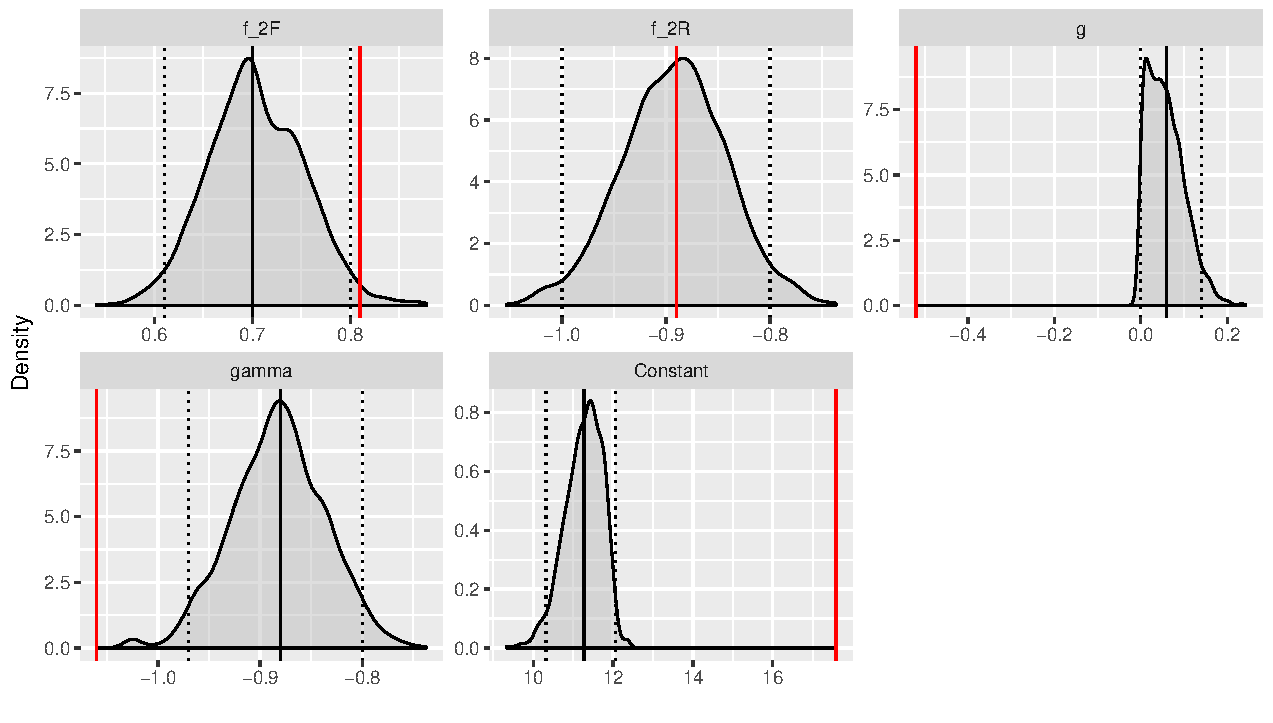
\includegraphics[width=\linewidth]{mkt1_v2r_post.pdf}
\caption{Posterior density function of elasticities w.r.t  $V_{2R}$ - Market 1}
\label{fig:mkt1_v2r_post}
\caption*{Source: Own work}
\end{figure} 

\textit{iv. Magnitude of estimates}

Analysing the magnitude and distributions of coefficients one can notice that the \textit{Full} fare is more sensitive to its own price, with mean -1.3, then the \textit{Reduced} fare, with mean -0.9. This difference may be reasonable if one considers the \textit{Reduced} fare as a basic service, accessible for everyone without time restrictions, whilst the \textit{Full} fare would offer a plus of convenient schedules in the peak hours. The price differentiation of \textit{Reduced} and \textit{Full} and its different sensitiveness to price would, therefore, be in accordance with economic theory which says that superfluous goods are more elastic than essential goods.

The magnitude of cross elasticities can be also interpreted by this rationale of basic and more convenient services. Therefore, the demand of \textit{Reduced} fare is more affected by variations in the price of the \textit{Full} fare than the contrary, which means that everything constant, when the \textit{Full} fare increases more passenger change for the \textit{Reduced} fare than vice-versa.

In which regards the GVA elasticity it is unexpectedly below 1 for the demand of \textit{Full}, with mean 0.7, and even more unexpected for the demand of \textit{Reduced}, being very close to zero. According to the PDFH, the GDP elasticities - for which GVA is assumed as an equivalent measure of income/wealth \citep[p.~ 4, Chapter B1]{pdfhv5}, are expected to be around $1.1$ \citep[p.~9, Chapter B1]{pdfhv5}. 

Irrespective of their magnitude, the fact that $g_{2F} > g_{2R}$ should be expected because there is a higher proportion of business trips in the \textit{Full} fare than in the \textit{Reduced}, for non-London long distance journeys \citep{pdfhv5}.

Lastly, the quality elasticity was very similar in both \textit{Full} and \textit{Reduced} demands, with mean -0.9 and similar standard deviation. These values are within the expected interval of -0.7 to -1.1, according to the PDFH \citep{pdfhv5}. However, business travellers are more sensitive to quality rather than price because ``it is undertaken at the time and at the expense of the employer" \citep[p.~1, Chapter A1]{pdfhv5}. Because of that, $\gamma_{2F} > \gamma_{2R}$ should be expected, which was not observed. 

% ====================================
% ====================================
% ====================================

\subsection{Market 2}

\textit{i. Autocorrelation and convergence}

In Market 2, the estimation was more complex. Both the $V_{2R}$ and $V_{2A}$ regressions demanded longer iterations (10,000 instead of 2,000) to converge with an acceptable amount of effective samples. Nevertheless, the estimation was successful, as demonstrated by the statistics in Table \ref{mkt2_T_autocorr_convergence}.

As in Market 1, there also were divergent transitions reported in all three regressions of Market 2. The previous interpretation applies.
% \\[3pt]

% latex table generated in R 3.3.2 by xtable 1.8-2 package
% Sat Aug  5 10:10:51 2017
\begin{table}[H]
\caption{Autocorrelation and Convergence Measures - Market 2}
\label{mkt2_T_autocorr_convergence}
\centering
\begin{tabular}{lrrrrrrrr}
\toprule 
 & \multicolumn{8}{c}{\textit{Dependent variable:}} \\ 
\cline{2-9} 
\\[-1.8ex] & \multicolumn{2}{c}{$ln \; V_{2F}$} & & \multicolumn{2}{c}{ $ln \; V_{2R}$} & &  \multicolumn{2}{c}{ $ln \; V_{2A}$}\\ 
\cline{2-3} \cline{5-6} \cline{8-9}
 & $\hat{R}$ & $n_{\text{eff}}$ & & $\hat{R}$ & $n_{\text{eff}}$  & & $\hat{R}$ & $n_{\text{eff}}$ \\ 
\hline \\[-1.8ex] 
  $f_{2F}$ & 1.0 & 405 & & 1.0 & 464 & & 1.0 & 529 \\ 
  $f_{2R}$ & 1.0 & 251 & & 1.0 & 414 & & 1.0 & 493 \\ 
  $f_{2A}$ & 1.0 & 614 & & 1.0 & 702 & & 1.0 & 634 \\ 
  $g$      & 1.0 & 315 & & 1.0 & 561 & & 1.0 & 555 \\ 
  $\gamma$ & 1.0 & 400 & & 1.0 & 525 & & 1.0 & 912 \\ 
  Constant & 1.0 & 310 & & 1.0 & 548 & & 1.0 & 500 \\
   \hline
   Iter    & \multicolumn{2}{c}{2,000} && \multicolumn{2}{c}{10,000} && \multicolumn{2}{c}{10,000} \\
   Thin    & \multicolumn{2}{c}{1} && \multicolumn{2}{c}{1} && \multicolumn{2}{c}{1} \\
   \bottomrule
\end{tabular}
\caption*{Source: Own work}
\end{table}


\textit{ii. OLS comparison}

A comparison between the Bayes and OLS estimates is presented in Table \ref{tbl:mkt2_T}. As expected, the all Bayesian coefficients have coherent signs. It has clearly improved the estimates since the OLS present four wrong sign elasticities.
% \\[3pt]

% latex table generated in R 3.3.2 by xtable 1.8-2 package
% Mon Jul 31 09:29:49 2017
\begin{table} [H]
\caption{Comparison of bayesian and SURE/OLS estimates - Martket 2}
\label{tbl:mkt2_T}
\centering
\begin{tabular}{rrrrrrrrrrr}
  \toprule 
 & \multicolumn{3}{c}{\textit{Bayes}} && \multicolumn{3}{c}{\textit{SURE/OLS}} \\ 
\cline{2-4} \cline{6-8} 
\\[-1.8ex] & $ln \; V_{2F}$ & $ln \; V_{2R}$ & $ln \; V_{2A}$ & & $ln \; V_{2F}$ & $ln \; V_{2R}$ & $ln \; V_{2A}$ \\ 
\hline \\[-1.8ex] 

  $f_{2F}$ & -1.29  & 0.04   & 0.05 & & -1.24 & 0.03$^{\dagger}$ & \cellcolor{gray!25}-0.18\\
  		     & (0.05) & (0.03) & (0.04) & & (0.06) & (0.06) & 0.10)\\ [0.2cm]
  $f_{2R}$ & 0.05   & -0.80  & 1.01 & &\cellcolor{gray!25}-0.06 & -0.60 & 1.03\\
  			   & (0.04) & (0.05) & (0.08) & & (0.08) & (0.08) & (0.13)\\ [0.2cm]
  $f_{2A}$ & 0.14   & 0.01   & -0.46 & &0.15 & \cellcolor{gray!25}-0.10 & -0.47 \\
           & (0.04) & (0.01) & (0.06) & &(0.04) & (0.04) & (0.06)\\ [0.2cm]
  $g$      & 1.68   & 0.96   & 0.29  & &1.75 & 0.39 & 0.66\\
  		     & (0.07) & (0.07) & (0.08) & &(0.11) & (0.10) & (0.17)\\ [0.2cm]
  $\gamma$ & -1.28  & -1.07  & -0.03 & &-1.23 & -1.21 & \cellcolor{gray!25}0.33\\
  			   & 0.06   & (0.06) & (0.03) & &(0.07) & (0.06) & (0.10)\\ [0.2cm]
  Constant & -0.28  & 5.46   & -0.61 & &-1.09$^{\dagger}$ & 11.72 & -5.53\\
  			   & (0.76) & (0.71) & (0.82) & &(1.15) & (1.09) & (1.77)\\ [0.2cm]
  % \hline
  % $\sigma$ & 1.36  & 1.29   & 2.10 &&&&\\
  % 		     & (0.01)& (0.01) & (0.02)&&&&\\
\bottomrule
Note: $^{\dagger}$ $p>0.1$
\end{tabular}
\caption*{Source: Own work}
\end{table}





% Additionally, it is possible to notice that the estimates, when not corrected, were very close to the OLS values, except for the GVA elasticities in the $ln V_{2R}$ and $ln V_{2A}$ regressions. The same is valid for the standard deviations. That may indicate that the constraints in the probability density functions' domains are being effective to estimate a coherent elasticity coefficient. To the other coefficients, the likelihood, which has similar results to the SURE/OLS estimates, prevails given the high number of observations.

\textit{iii. Uncertainty}

% 1.
Figures \ref{fig:mkt2_v2f_post}, \ref{fig:mkt2_v2r_post} and \ref{fig:mkt2_v2a_post} illustrate the probability densities of the estimated elasticities coefficients. The elements in the graphs remain as explained for Market 1.

% 2.
Again, the small standard deviations were very important in constraining the range of credible values for the estimates in the decimal, even centesimal, scale. The HDI was generally satisfactorily small with the exception of two elasticities, with respect the demand $V_{2A}$. Nevertheless, they were very close to 0.30.

% 3a.
With respect to the $V_{2F}$ demand, Figure \ref{fig:mkt2_v2f_post}, all HDI were in generally satisfactorily small, from 0.14 to 0.28, demonstrating low uncertainty since the credible values are concentrated in small intervals. It is observed that the fare elasticities had the smaller HDI - 0.17, 0.14 and 0.15 for \textit{Full}, \textit{Reduced} and \textit{Advance}, respectively, in opposition to the $g$ and $\gamma$ which were above 0.20. Detailed information of the HDI is presented in the Appendix \ref{apd:bayes_hdi}. 

% 3b.
The OLS estimates lied inside the HDI interval, which indicates that the OLS estimates can be deemed credible values according to the Bayesian estimation. An exception is made for the $f_{2R}$, for which it should already be expected since its OLS estimate was on an unfeasible domain. 

% 3c.
All elasticities distributions are bell-shaped curves, although with some deformity, except for the $f_{2R}$, skewed towards the left with an abrupt cut at zero. It is noticeable that this is the sign-reverted elasticity, which may indicate that the constraint to a positive domain was an actual barrier. What apparently happens is that, because the likelihood considers feasible values on the negative side but the prior does not allow this domain, they tend to agree until zero, so samples are extracted until the limit of the constraint. Beyond that point, they clash, and since the prior assumes zero probability for those values, it is reflected in the posterior distribution. Indeed this may explain the warnings of divergent transitions. 

\begin{figure}[H]
\centering
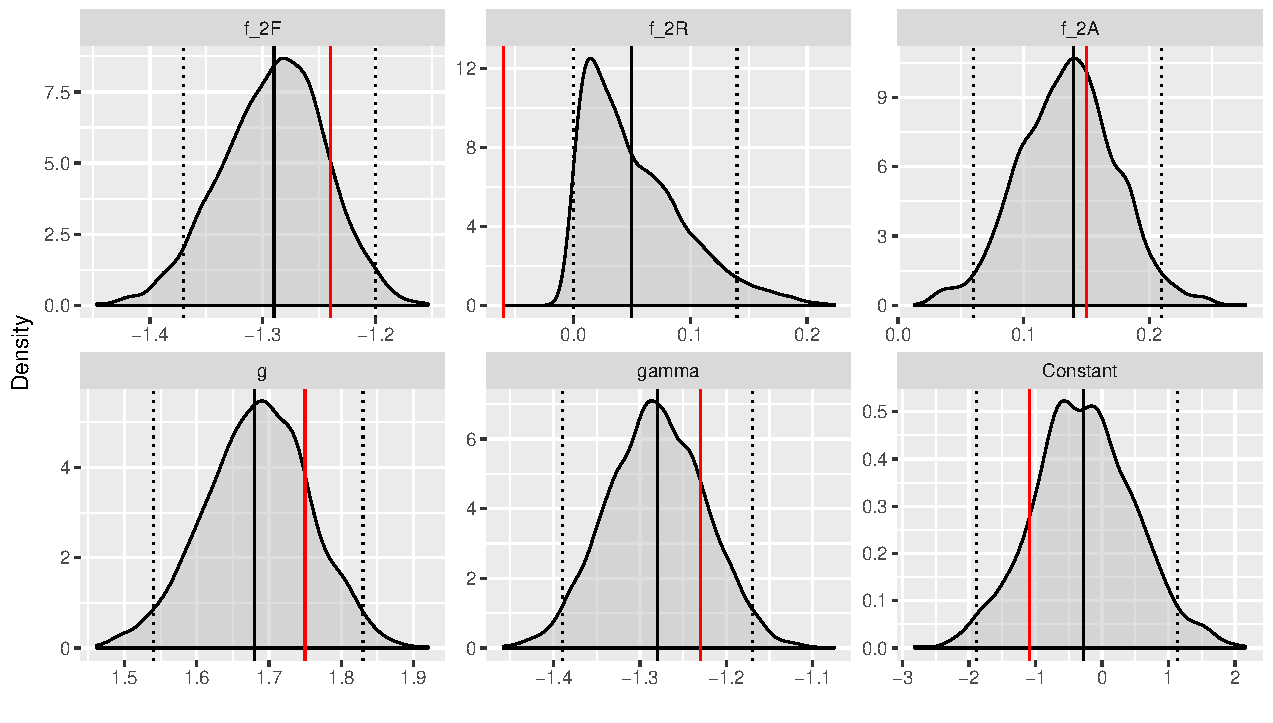
\includegraphics[width=\linewidth]{mkt2_v2f_post.pdf}
\caption{Posterior density function of elasticities w.r.t $V_{2F}$ - Market 2}
\label{fig:mkt2_v2f_post}
\caption*{Source: Own work}
\end{figure} 

% 3a.
With respect to the demand $V_{2R}$, Figure \ref{fig:mkt2_v2r_post}, there were very short HDI intervals, as for $f_{2F}$ and $f_{2A}$, 0.09 and 0.03 respectively, indicating a very precise estimation. The other fare elasticity can also be considered with low HDI, ranging 20\%. Again the $g$ and $\gamma$ had higher intervals. Detailed information of the HDI is presented in the Appendix \ref{apd:bayes_hdi}. 

% 3b.
The OLS estimation lied inside the HDI interval only for the $f_{2F}$ elasticity, which indicates big discrepancies between the Bayesian and frequentist's outputs.

% 3c.
Again, the sign-reversed coefficient, $f_{2A}$, had its distribution finishing abruptly at the zero bound. The cut at zero also appears for the $f_{2F}$ elasticity. Here it is also applied the interpretation of the sharp edge made for the $f_{2R}$, with respect to the demand $V_{2F}$.

\begin{figure}[H]
\centering
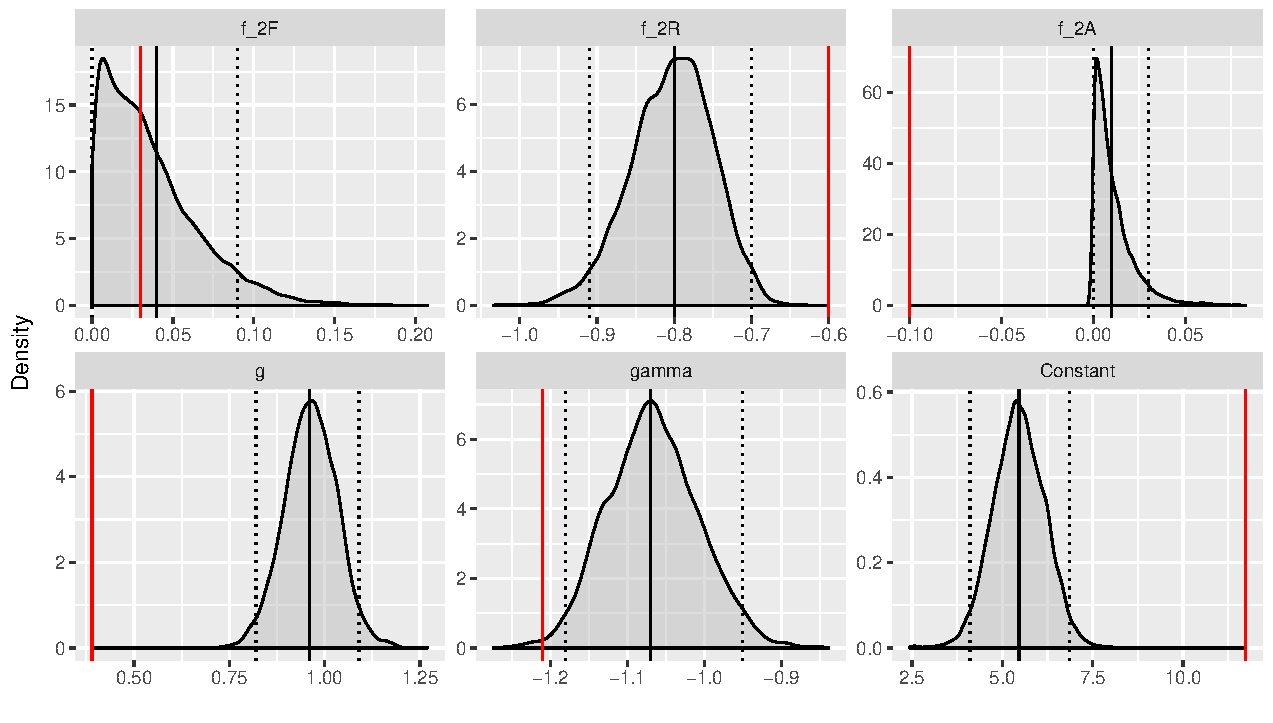
\includegraphics[width=\linewidth]{mkt2_v2r_post.pdf}
\caption{Posterior density function of elasticities w.r.t $V_{2R}$ - Market 2}
\label{fig:mkt2_v2r_post}
\caption*{Source: Own work}
\end{figure} 

% 3a.
With respect to the demand $V_{2A}$, Figure \ref{fig:mkt2_v2a_post}, the HDI's range was satisfactorily small for $f_{2F}$, $f_{2A}$ and $\gamma$, with a surprisingly precise estimate ranging only 0.08. For the other elasticities, however, they were above 0.30, even though they are close to it. It must be highlighted that one can always trade-off certainty for precision, which means that reducing the target probability of HDI will also provide more precise intervals. Detailed information of the HDI is presented in the Appendix \ref{apd:bayes_hdi}. 

% 3b
The analysis of the position of OLS estimates relatively to the HDI shows divergences between the two estimation methods. Only for $f_{2R}$ and $f_{2A}$ the OLS mean lies inside the HDI.

% 3c
Again, the sign-reversed coefficients, $f_{2F}$ and $g$ presented a sharp edge at the zero value. The previous interpretation applies.

\begin{figure}[H]
\centering
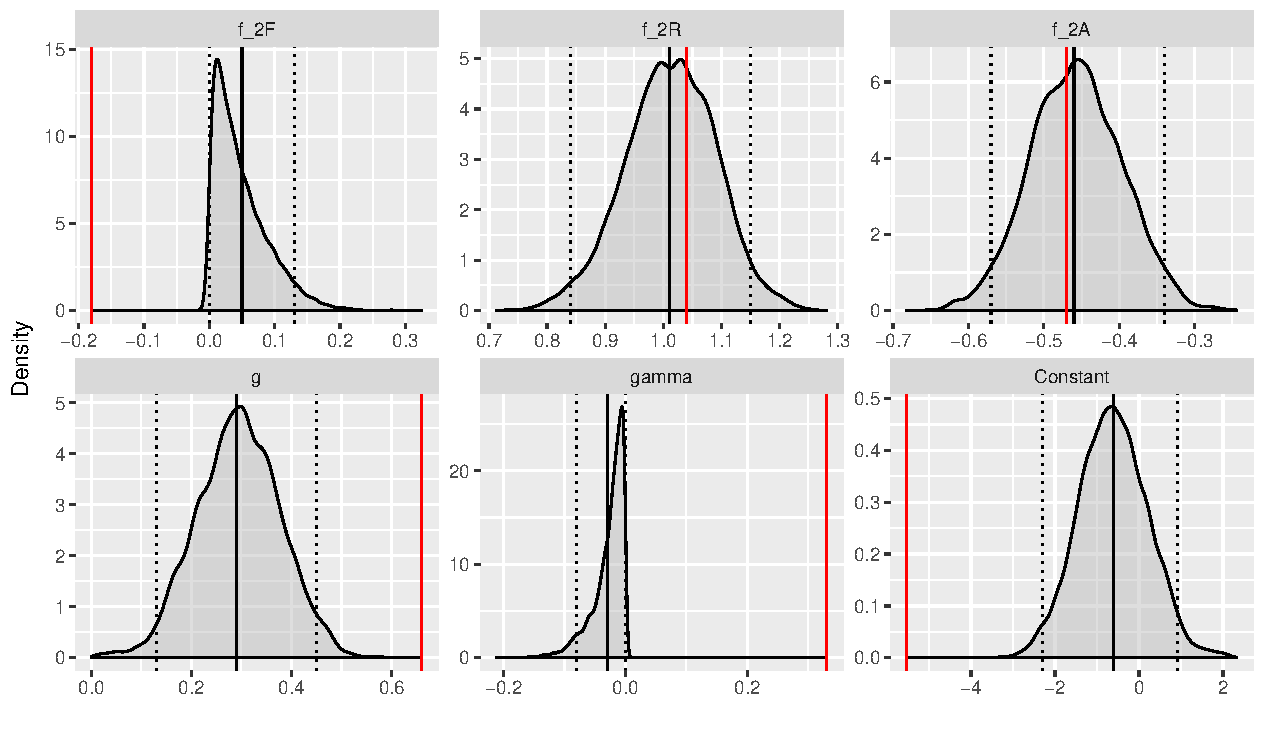
\includegraphics[width=\linewidth]{mkt2_v2a_post.pdf}
\caption{Posterior density function of elasticities w.r.t $V_{2A}$ - Market 2}
\label{fig:mkt2_v2a_post}
\caption*{Source: Own work}
\end{figure} 

% \\[3pt]

\textit{iv. Magnitude of estimates}

% 1.
Analysing of the magnitude of coefficients, the most sensitive fare with regard its own price is \textit{Full}, with mean -1.29, followed by the \textit{Reduced}, with mean -0.80. These values are close to the estimates in Market 1, which is interesting since both do not have \textit{First Class} tickets. The \textit{Advance} fare presented a lower own elasticity, -0.46.

% 2.
Regarding the cross elasticities, for the \textit{Full} fare they were very small - 0.04 and 0.05, indicating a very low impact in the other ticket demands. 

Conversely, for the \textit{Reduced}, a notably high cross elasticity of 1.01 - higher than the own elasticity, was computed with respect to the \textit{Advance} demand. The other cross elasticity was a very small effect - -0.05.

Lastly, for the \textit{Advance} fare, both cross elasticities were considerably small effects - 0.014 and 0.01.

% % these high cross elasticities of $f_{2R}$ with respect the demand of 2A tickets may be justified because reduced demand is more related to leisure passengers [CITE SOMETHING], they are more willing to adapt behaviour if necessary. Therefore, facing an increase in prices, a passenger will plan their trips in advance - which causes the migration to the 2A  demand. Conversely, if prices go down, there is no value in committing themselves with anticipated plans of a trip. 

% % If the volume of \textit{Reduced} tickets were equivalent to the volume of \textit{Advance} one should expect the $f_{2A}$ coefficient in the $ln V_{2R}$ regression to be equivalent, however, as long as the \textit{Advance} tickets are quota controlled... (see also market share of tickets). [IS IT TRUE? SEE SLUTISKY SIMMETRY].

% 3.
The GVA elasticity in this market are significantly higher than in the Market 1, which is difficult to interpret. However, a sign of consistency is noticed since there still is the pattern of the GVA affecting more the \textit{Full} demand, whose mean is 1.68, then the \textit{Reduced}, whose mean is 0.96. For the \textit{Advance} demand the elasticity was of 0.29, but because the advance fares are a mix of promotional fares from both \textit{Full} and \textit{Reduced} it is difficult to interpret it as well.

% 4.
Lastly, the GJT elasticities were also higher than in Market 1, which is difficult to reasonably interpret. Additionally, they did not follow the same pattern from the previous market, in which they coefficients had very similar means. Instead, for the \textit{Full} demand the mean was deemed as -1.28, and for the \textit{Reduced} it was -1.07.

It is interesting, however, that the GJT elasticity of the \textit{Advance} ticket has a very tight distribution close to zero, being far from the expected interval of -0.7 and -1.1 \citep{pdfhv5} without an explicit reason.

% can be interpreted due to the nature of that fare. Because it is a mix of promotional fares from both \textit{Full} and \textit{Reduced} passengers are not sensitive to the quality of the service, since buying an advanced ticket is only a matter of discount for experiencing either one or other service. 
% ==================================
% ==================================
% ==================================

\subsection{Market 3}

\textit{i. Autocorrelation and convergence}

In the third market, the estimation was more complex than in previous markets. The estimation of $V_{2F}$, $V_{2R}$ and $V_{2A}$ demanded longer iterations (10,000 instead of 2,000) to converge with an acceptable amount of effective samples. Additionally, to reduce autocorrelation, the thinness was increased to 5. The resultant estimation was successful, with low autocorrelation, as shown in Table \ref{mkt3_T_autocorr_convergence_SCOTYORK}.

As in Market 1 and 2, there also were divergent transitions reported in all four regressions of Market 3. The previous interpretation applies.

% latex table generated in R 3.3.2 by xtable 1.8-2 package
% Sat Aug  5 10:10:51 2017
\begin{table}[ht]
\caption{Autocorrelation and Convergence Measures - Market 3}
\label{mkt3_T_autocorr_convergence_SCOTYORK}
\centering
\begin{tabular}{lrrrrrrrrrrr}
\toprule 
 & \multicolumn{11}{c}{\textit{Dependent variable:}} \\ 
\cline{2-12} 
\\[-1.8ex] & \multicolumn{2}{c}{$ln \; V_{1N}$} & &\multicolumn{2}{c}{$ln \; V_{2F}$} & & \multicolumn{2}{c}{ $ln \; V_{2R}$} & &  \multicolumn{2}{c}{ $ln \; V_{2A}$}\\ 
\cline{2-3} \cline{5-6} \cline{8-9} \cline{11-12}
 & $\hat{R}$ & $n_{\text{eff}}$ & & $\hat{R}$ & $n_{\text{eff}}$  & & $\hat{R}$ & $n_{\text{eff}}$ & & $\hat{R}$ & $n_{\text{eff}}$ \\  
\hline \\[-1.8ex] 
  $f_{1N}$ & 1.0 & 2712 & & 1.0 & 492 & & 1.0 & 826 & & 1.0 & 939 \\
  $f_{2F}$ & 1.0 & 2350 & & 1.0 & 278 & & 1.0 & 637 & & 1.0 & 1031\\
  $f_{2R}$ & 1.0 & 2203 & & 1.0 & 205 & & 1.0 & 561 & & 1.0 & 948 \\
  $f_{2A}$ & 1.0 & 3000 & & 1.0 & 294 & & 1.0 & 678 & & 1.0 & 1187\\
  $g$      & 1.0 & 2128 & & 1.0 & 147 & & 1.0 & 376 & & 1.0 & 668 \\
  $\gamma$ & 1.0 & 2708 & & 1.0 & 367 & & 1.0 & 559 & & 1.0 & 945 \\
  Constant & 1.0 & 2130 & & 1.0 & 140 & & 1.0 & 409 & & 1.0 & 756 \\
   \hline
   Iter   & \multicolumn{2}{c}{2,000} && \multicolumn{2}{c}{10,000} && \multicolumn{2}{c}{10,000} && \multicolumn{2}{c}{10,000} \\
   Thin   & \multicolumn{2}{c}{1} && \multicolumn{2}{c}{5} && \multicolumn{2}{c}{1} && \multicolumn{2}{c}{5} \\
   \bottomrule
\end{tabular}
\caption*{Source: Own work}
\end{table}
% \\[3pt]

\textit{ii. OLS comparison}

A comparison between the Bayes and OLS estimates is presented in Table \ref{tbl:mkt3_T_SCOTYORK}. As expected, the all Bayesian coefficients have coherent signs. It has clearly improved the estimates since the OLS present four wrong sign elasticities.

% latex table generated in R 3.3.2 by xtable 1.8-2 package
% Mon Jul 31 09:29:49 2017
\begin{table}
\caption{Comparison of elasticities estimates - Martket 3}
\label{tbl:mkt3_weak_SCOTYORK}
\centering
\begin{tabular}{lrrrrrrrrrr}
  \toprule 
 & \multicolumn{4}{c}{\textit{Bayes}} && \multicolumn{4}{c}{\textit{SURE/OLS}} \\ 
\cline{2-5} \cline{7-10} 
\\[-1.8ex] & $ln \; V_{1N}$ & $ln \; V_{2F}$ & $ln \; V_{2R}$ & $ln \; V_{2A}$ & & $ln \; V_{1N}$ & $ln \; V_{2F}$ & $ln \; V_{2R}$ & $ln \; V_{2A}$ \\ 
\hline \\[-1.8ex] 

$f_{1N}$ & -0.82  & \cellcolor{gray!25}-0.42  & \cellcolor{gray!25}-0.41  & \cellcolor{gray!25}-0.47   && -0.84 & \cellcolor{gray!25}-0.43 & \cellcolor{gray!25}-0.44 & \cellcolor{gray!25}-0.50 \\
         & (0.06) & (0.05) & (0.05) & (0.07)  && (0.06) & (0.05) & (0.05) & (0.07) \\ [0.2cm]
$f_{2F}$ & 1.03   & -1.13  & 0.20   & 1.13    && 1.03 & -1.12 & 0.23 & 1.07 \\
         & (0.08) & (0.07) & (0.07) & (0.10)  && (0.09) & (0.07) & (0.07) & (0.10) \\ [0.2cm]
$f_{2R}$ & 1.73   & \cellcolor{gray!25}-0.06  & \cellcolor{gray!25}0.23   & 2.23    && 1.80 & \cellcolor{gray!25}-0.04 & \cellcolor{gray!25}0.34 & 2.28 \\ 
         & (0.10) & (0.09) & (0.08) & (0.13)  && (0.11) & (0.09) & (0.09) & (0.13) \\ [0.2cm]
$f_{2A}$ & 0.44   & 0.33   & 0.19   & -0.42   && 0.43 & 0.33 & 0.15 & -0.39 \\
         & (0.06) & (0.05) & (0.05) & (0.07)  && (0.06) & (0.05) & (0.05) & (0.07) \\ [0.2cm]
$g$      & 1.52   & 1.78   & 1.29   & 1.11    && 1.50 & 1.66 & 0.80 & 1.54 \\ 
         & (0.08) & (0.07) & (0.07) & (0.08)  && (0.11) & (0.09) & (0.09) & (0.13) \\ [0.2cm]
$\gamma$ & -3.25  & -1.57  & -2.17  & -2.06   && -3.30 & -1.60 & -2.31 & -2.01 \\ 
         & (0.08) & (0.06) & (0.06) & (0.09)  && (0.082) & (0.07) & (0.07) & (0.10) \\ [0.2cm]
Constant & 0.23   & 1.51   & 6.15   &  -2.21  && 0.62$^{\dagger}$ & 2.85 & 11.66 & -6.72 \\ 
         & (0.78) & (0.73) & (0.70) & (0.82)  && (1.23) & (1.00) & (0.95) & (1.45) \\ [0.2cm]
\bottomrule
\multicolumn{3}{l}{Note: $^{\dagger}$ $p>0.1$}
\end{tabular}
\caption*{Source: Own work}
\end{table}



\textit{iii. Uncertainty}

% 1.
Figures \ref{fig:mkt3_v1n_SCOTYORK_post}, \ref{fig:mkt3_v2f_SCOTYORK_post}, \ref{fig:mkt3_v2r_SCOTYORK_post} and \ref{fig:mkt3_v2a_SCOTYORK_post} illustrate the probability densities of the estimated elasticities coefficients. The elements in the graphs remain as previously explained. 

% 2.
In this estimation, the standard deviations were not satisfactorily small as in the previous markets. Neither was the amplitude of HDI intervals: for 7 out of 24 elasticities it was above 0.30. As discussed before, is always possible to trade-off certainty for precision. Nevertheless, in general, the estimation clearly lost in quality in this market. 

% It emerges, therefore, a trade-off between the precision of the HDI interval and probability of the interval values, since one may reduce the HDI' probability coverage, reducing the HDI for 80\%, for instance, in order to reduce the range between the smallest and the higher credible values.

\begin{figure}[H]
\centering
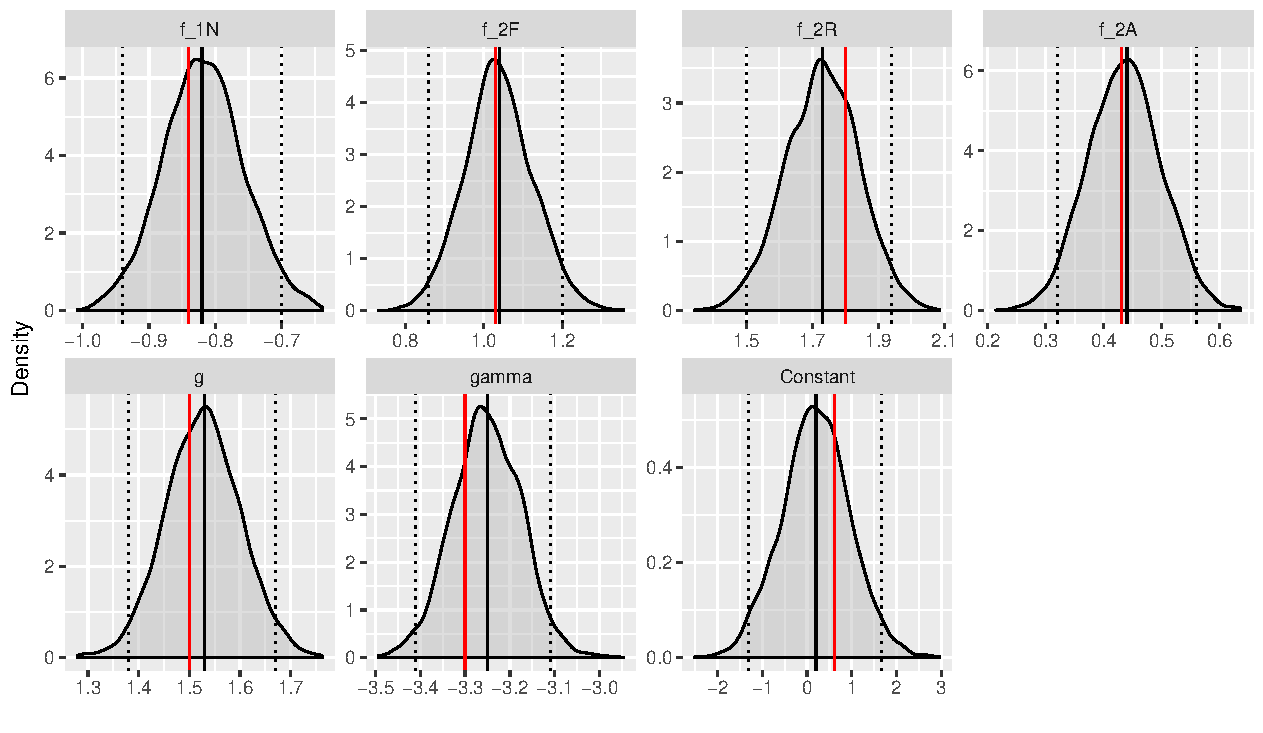
\includegraphics[width=\linewidth]{mkt3_v1n_SCOTYORK_post.pdf}
\caption{Posterior density function of elasticities w.r.t $V_{1N}$ - Market 3}
\label{fig:mkt3_v1n_SCOTYORK_post}
\caption*{Source: Own work}
\end{figure} 

% 3a.
With respect to the $V_{1N}$ demand, Figure \ref{fig:mkt3_v1n_SCOTYORK_post}, half of the coefficients had HDI's amplitude below 0.30 - $f_{1N}$, $g$ and $\gamma$, and half were above this value - $f_{2F}$, $f_{2R}$ and $\gamma$, achieving up to 0.43. Detailed information of the HDI is presented in the Appendix \ref{apd:bayes_hdi}. 

% 3bc
As one may notice, for this estimation, there were no discrepancies between the OLS mean estimates and the Bayesian ones - all were very close. This may have occurred because the OLS estimates have already had correct algebraic signs. Therefore, the constraints applied to the prior did not represent actually barriers to help to shape the posterior distributions. Indeed, there were no sharp edges in any distribution. 

Since the constraint was not effective, the priors become simply non-informative priors, and because of the large number of observations, the likelihood prevails, causing the estimation to be similar to the OLS. Indeed, all OLS estimates are lying inside the HDI interval.

The inefficiency of the prior may also explain the large standard deviations. As one may recover from Chapter \ref{chp:lit-rev}, in the presence of high correlation of variables, strong priors are important because defining the boundaries of one covariant automatically shapes the correlated one. Thus, the mixed and blurred joint effect of two correlated variables takes a cut-off point.

\begin{figure}[H]
\centering
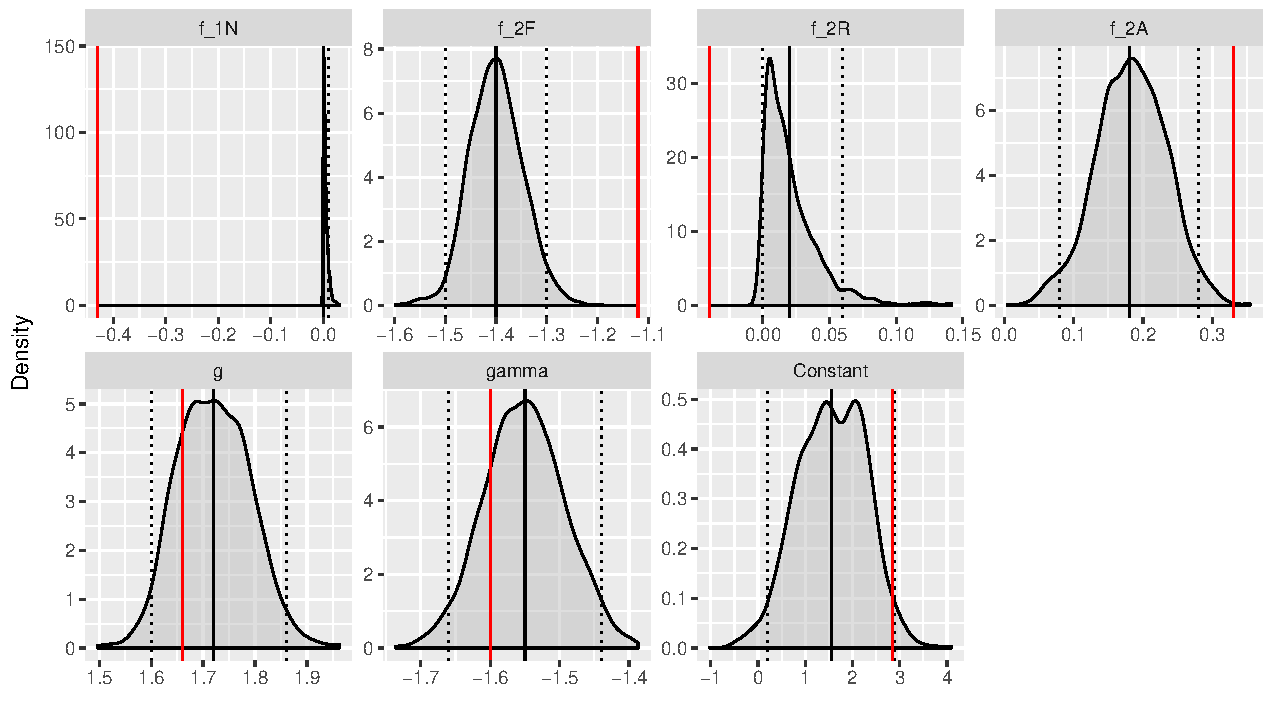
\includegraphics[width=\linewidth]{mkt3_v2f_SCOTYORK_post.pdf}
\caption{Posterior density function of elasticities w.r.t $V_{2F}$ - Market 3}
\label{fig:mkt3_v2f_SCOTYORK_post}
\caption*{Source: Own work}
\end{figure} 

% 3a
With respect to the $V_{2F}$ demand, Figure \ref{fig:mkt3_v2f_SCOTYORK_post}, the elasticities' HDI were satisfactorily small. The sign-reversed coefficients $f_{1N}$ and $f_{2N}$notably presented HDI with very small amplitude, 0.01 and 0.06, respectively. Detailed information of the HDI is presented in the Appendix \ref{apd:bayes_hdi}. 

% 3b
With these short HDI intervals, the OLS estimates lied out of the range of credible values for all estimates, but $g$. This shows that the precision of bayesian estimates was enough to distinguish even OLS estimates that already have correct algebraic signs from being credible values.

% 3c
It is noticeable that, once again, for the sign-reversed coefficients, the shape of the posterior distribution is skewed towards the zero value, showing that the imposition of constraint was fundamental to avoid the wrong sign estimates indicated by the likelihood.

% 3a
With respect to the $V_{2R}$ demand, Figure \ref{fig:mkt3_v2r_SCOTYORK_post}, the elasticities' HDI were again satisfactorily small. It is noticeable that, as in the previous model, the $f_{1N}$ elasticity was very close to zero HDI's range of 0.02. Detailed information of the HDI is presented in the Appendix \ref{apd:bayes_hdi}. 

% 3b
The OLS estimates lied out of the credible values of for $g$ and $\gamma$, besides the sign-reversed coefficients, for which it should already be expected. 

% 3c
Also, similarly to the last model, the sign-reversed coefficients had skewed distributions towards the zero constraints. A similar interpretation is applicable in this regard.

\begin{figure}[H]
\centering
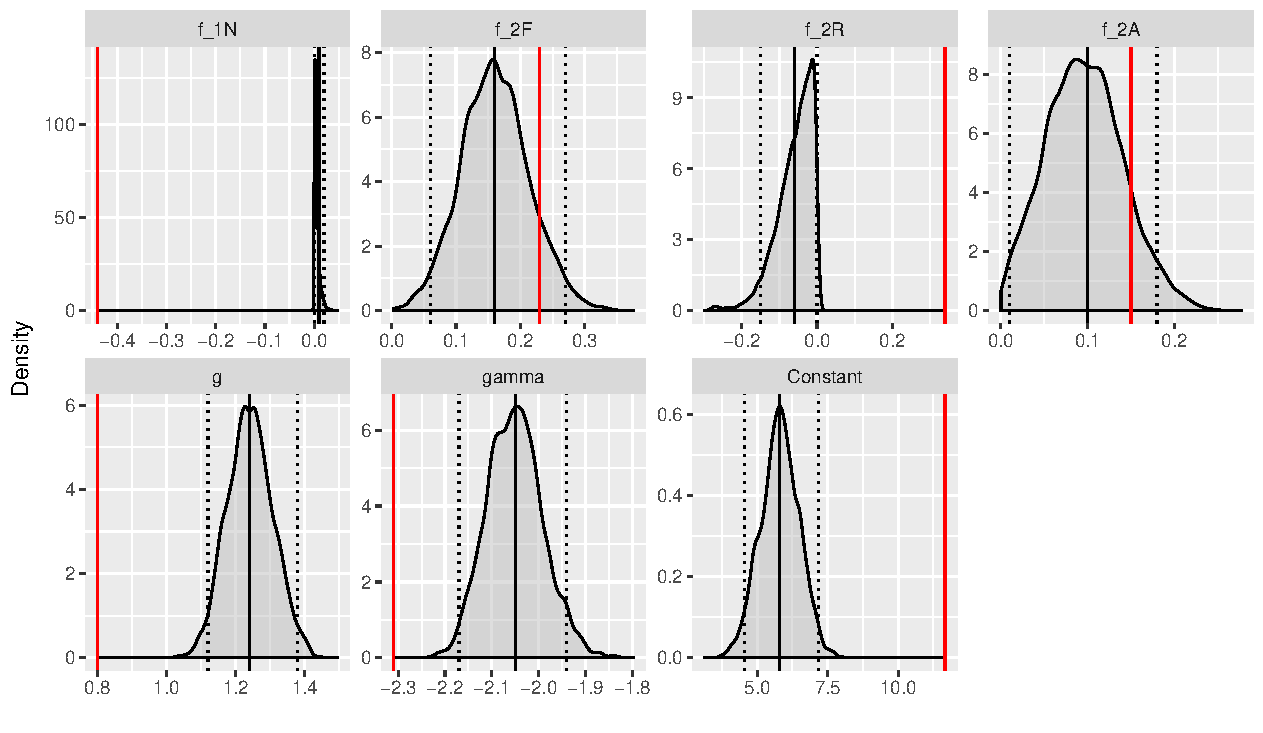
\includegraphics[width=\linewidth]{mkt3_v2r_SCOTYORK_post.pdf}
\caption{Posterior density function of elasticities w.r.t $V_{2R}$ - Market 3}
\label{fig:mkt3_v2r_SCOTYORK_post}
\caption*{Source: Own work}
\end{figure} 

\begin{figure}[H]
\centering
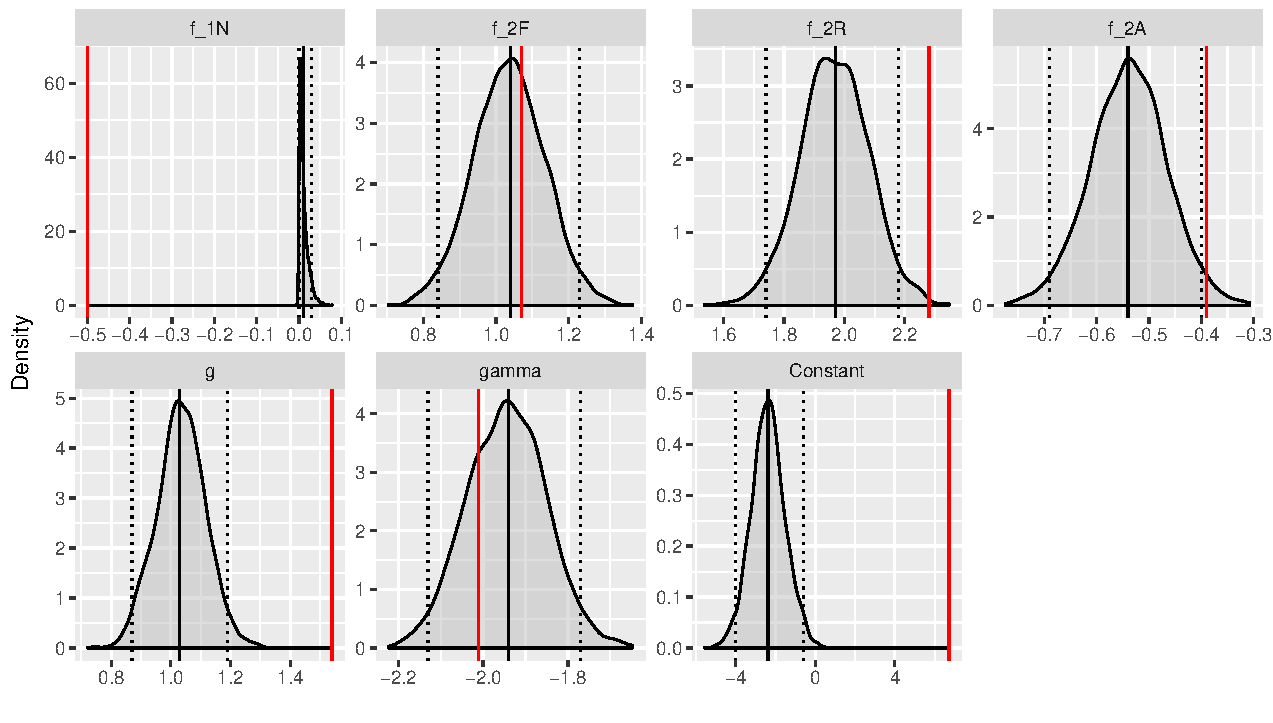
\includegraphics[width=\linewidth]{mkt3_v2a_SCOTYORK_post.pdf}
\caption{Posterior density function of elasticities w.r.t $V_{2A}$ - Market 3}
\label{fig:mkt3_v2a_SCOTYORK_post}
\caption*{Source: Own work}
\end{figure} 

% 3a
With respect to the $V_{2A}$ demand, Figure \ref{fig:mkt3_v2a_SCOTYORK_post}, the HDI are again presenting ranges above 0.30 up to 0.44 ($f_{2R}$). excepted for $f_{1N}$ and $f_{2A}$. The $f_{2A}$ was at the edge, with 029. Conversely, it is noticeable that the $f_{1N}$, as in the last model, it presented a very short HDI of 0.03. Detailed information of the HDI is presented in the Appendix \ref{apd:bayes_hdi}. 

% 3b
Even though the large HDI intervals, the OLS estimates lied out of the credible values for the $f_{1N}$, which was already expected since the OLS estimates were in the wrong domain, $f_{2R}$, $f_{2A}$ and $g$. 

% 3c
Once again, the sign-reversed coefficient had skewed distributions towards the zero constraints. A similar interpretation is applicable in this regard.
\\[3pt]

\textit{iv. Magnitude of estimates}

% 1.
Analysing the magnitude of coefficients, the most sensitive fare with regard its own price is the \textit{Full}, with mean -1.4, followed by the \textit{First Class}, with mean -0.82, \textit{Advance}, with mean -0.46 and \textit{Reduced}, with a very low mean of -0.06. Notably, the \textit{Full} fare remains very elastic in this market.

% 2.
Regarding the cross elasticities, there were very extreme values - small effects very close to zero and high cross elasticities, bigger than 1. 

Some notable observations deserves to be highlighed: the virtually null cross elasticities for the \textit{First Class} for all demands; the high cross elasticities of the \textit{Full} fare with respect to \textit{First Class} and \textit{Advance}, 1.04 for both and the also high effects of the \textit{Reduced} fare with respect to the \textit{First Class} and \textit{Advanced} demands - 1.73 and 1.97, respectively. That may deserve further investigation. Eventually other constraints may be applied to test the propability of these elasticities being smaller.

% 3.
The GVA elasticity was above unit for all type of demands, which may be deemed reasonable since PDFH states a general expected value of 1.1 \citep[p.~9, Chapter B1]{pdfhv5} and also considers that ``the elasticities to GDP (...) can be expected to vary by ticket type" \citep[p.~7, Chapter B2]{pdfh}. It worths noticing that $g_{2F} > g_{2R}$, which is consistent with the fact that the percentage of business journeys is higher in \textit{Full} tickets. However, it is intriguing that $g_{1N} < g_{2F}$ because \textit{First class} is usually associated with business journeys. Nevertheless, it should be highlighted that the 1N fare aggregates \textit{Full}, \textit{Reduced} and \textit{Advance} tickets from the first class. In other words, 1N mixes the types of fares for which PDFH have stated the shares of trip purposes - there is only differentiation of trip purpose between \textit{Full} and \textit{Reduced}, making it unclear to judge the elasticity magnitude by this terms.

% 4.
For the GJT effects, the elasticities were considerably high:  from -1.55, for the \textit{Full} demand, to -3.25, for the \textit{First Class}. Even though there is the same GVA's reservation that states that elasticities can be expected to vary by ticket type \citep{pdfh}, it is markedly above general interval expected by PDFH - -0.7 to -1.1 \citep{pdfhv5}. 

It is remarkable that the most quality sensitive fare is the \textit{First Class}, which is reasonable since the first class is a quality differentiation, but the relative magnitude of the others are difficult to interpret.

% ==================================
% ==================================
% ==================================

\subsection{Market 4}

\textit{i. Autocorrelation and convergence}

The estimation was complex again, as it was in the third. Except for the $V_{2R}$, the models demanded longer iterations (10,000 instead of 2,000) to converge with an acceptable amount of effective samples. Additionally, to reduce autocorrelation, the thinness was increased to 5 for $V_{1A}$ and $V_{2F}$. Nevertheless, the estimation was successful, as demonstrated by the statistics in Table \ref{mkt4_T_autocorr_convergence_SCOTYORK}.

As in all previous markets, there also were divergent transitions reported in all regressions of Market 4. The previous interpretation applies.

% latex table generated in R 3.3.2 by xtable 1.8-2 package
% Sat Aug  5 10:10:51 2017
\begin{table}[H]
\caption{Autocorrelation and Convergence Measures - Market 4}
\label{mkt4_T_autocorr_convergence_SCOTYORK}
\centering
\begin{tabular}{lrrrrrrrrrrrrrrrrrrrr}
\toprule 
 & \multicolumn{17}{c}{\textit{Dependent variable:}} \\ 
\cline{2-21} 
\\[-1.8ex] & \multicolumn{2}{c}{$ln \; V_{1F}$} & & \multicolumn{2}{c}{$ln \; V_{1R}$} & & \multicolumn{2}{c}{$ln \; V_{1A}$} & & \multicolumn{2}{c}{$ln \; V_{2F}$} & & \multicolumn{2}{c}{ $ln \; V_{2R}$} & &  \multicolumn{2}{c}{ $ln \; V_{2A}$}\\ 
\cline{2-3} \cline{5-6} \cline{8-9} \cline{11-12} \cline{14-15} \cline{17-18}
 & $\hat{R}$ & $n_{\text{eff}}$ & & $\hat{R}$ & $n_{\text{eff}}$  & & $\hat{R}$ & $n_{\text{eff}}$ & & $\hat{R}$ & $n_{\text{eff}}$ & & $\hat{R}$ & $n_{\text{eff}}$ & & $\hat{R}$ & $n_{\text{eff}}$\\  
\hline \\[-1.8ex] 
  $f_{1F}$ & 1.0 & 707 & & 1.0 & 373 & & 1.0 & 622 & & 1.0 & 173 & & 1.0 & 98 & & 1.0 & 408 \\
  $f_{1R}$ & 1.0 & 534 & & 1.0 & 273 & & 1.0 & 548 & & 1.0 & 186 & & 1.0 & 339 & & 1.0 & 473 \\
  $f_{1A}$ & 1.0 & 663 & & 1.0 & 409 & & 1.0 & 632 & & 1.0 & 139 & & 1.0 & 225 & & 1.0 & 435 \\
  $f_{2F}$ & 1.0 & 826 & & 1.0 & 260 & & 1.0 & 739 & & 1.0 & 147 & & 1.0 & 278 & & 1.0 & 515 \\
  $f_{2R}$ & 1.0 & 668 & & 1.0 & 308 & & 1.0 & 527 & & 1.0 & 133 & & 1.0 & 206 & & 1.0 & 284 \\
  $f_{2A}$ & 1.0 & 251 & & 1.0 & 354 & & 1.0 & 799 & & 1.0 & 121 & & 1.0 & 213 & & 1.0 & 410 \\
  $g$      & 1.0 & 442 & & 1.0 & 311 & & 1.0 & 507 & & 1.0 & 95  & & 1.0 & 211 & & 1.0 & 221 \\
  $\gamma$ & 1.0 & 596 & & 1.0 & 292 & & 1.0 & 533 & & 1.0 & 149 & & 1.0 & 268 & & 1.0 & 320 \\
  Const. & 1.0 & 485 & & 1.0 & 280 & & 1.0 & 469 & & 1.0 & 103  & & 1.0 & 197 & & 1.0 & 404 \\
  \hline
  Iter     & \multicolumn{2}{c}{10,000} && \multicolumn{2}{c}{10,000} && \multicolumn{2}{c}{10,000} && \multicolumn{2}{c}{10,000} && \multicolumn{2}{c}{2,000} && \multicolumn{2}{c}{10,000}\\
  Thin     & \multicolumn{2}{c}{1} && \multicolumn{2}{c}{1} && \multicolumn{2}{c}{5} && \multicolumn{2}{c}{5} && \multicolumn{2}{c}{1} && \multicolumn{2}{c}{1}\\
   \bottomrule
\end{tabular}
\caption*{Source: Own work}
\end{table}

\vspace{-2em}
\textit{ii. OLS comparison}

A comparison between the Bayes and OLS estimates is presented in Table \ref{tbl:mkt4_T_SCOTYORK}. As expected, all Bayesian coefficients have coherent signs. It clearly improved the estimates, reverting the ten wrong sign elasticities from the OLS estimates.
% \\[3pt]

\begin{landscape}
% latex table generated in R 3.3.2 by xtable 1.8-2 package
% Mon Jul 31 09:29:49 2017
\begin{table} [H]
\caption{Comparison of bayesian and SURE/OLS estimates - Martket 4}
\label{tbl:mkt4_T_SCOTYORK}
\centering
\begin{tabular}{lrrrrrrrrrrrrr}
  \toprule 
 & \multicolumn{6}{c}{\textit{Bayes}} && \multicolumn{6}{c}{\textit{SURE/OLS}} \\ 
\cline{2-7} \cline{9-14} 
\\[-1.8ex] & $ln \; V_{1F}$ & $ln \; V_{1R}$ & $ln \; V_{1A}$ & $ln \; V_{2F}$ & $ln \; V_{2R}$ & $ln \; V_{2A}$ & & $ln \; V_{1F}$ & $ln \; V_{1R}$ & $ln \; V_{1A}$ & $ln \; V_{2F}$ & $ln \; V_{2R}$ & $ln \; V_{2A}$ \\ 
\hline \\[-1.8ex] 

$f_{1F}$ & -1.02  & 0.04   & 1.10   & 0.02   & 0.16   & 0.46   && -0.94   & \cellcolor{gray!25}-0.09$^{\dagger}$   & 1.20    & \cellcolor{gray!25}-0.50   & 0.01$^{\dagger}$    & 0.54 \\ 
         & (0.19) & (0.04) & (0.19) & (0.02) & (0.12) & (0.20) && (0.22)  & (0.27)  & (0.27)  & (0.20)  & (0.19)  & (0.26) \\ [0.08cm]
$f_{1R}$ & 0.05   & -0.49  & 0.02   & 0.01   & 0.21   & 0.03   && 0.06$^{\dagger}$    & -0.43   & \cellcolor{gray!25}-0.25   & \cellcolor{gray!25}-0.14   & 0.22    & \cellcolor{gray!25}-0.11 \\ 
         & (0.04) & (0.07) & (0.02) & (0.01) & (0.05) & (0.03) && (0.06)  & (0.08)  & (0.08)  & (0.06)  & (0.05)  & (0.07) \\ [0.08cm]
$f_{1A}$ & 0.24   & 0.02   & -0.09  & 0.04   & 0.39   & 0.80   && 0.28    & \cellcolor{gray!25}-0.99   & \cellcolor{gray!25}0.09$^{\dagger}$    & \cellcolor{gray!25}0.33    & 0.44    & 0.88 \\ 
         & (0.11) & (0.02) & (0.07) & (0.03) & (0.09) & (0.13) && (0.125) & (0.151) & (0.154) & (0.114) & (0.108) & (0.147) \\ [0.08cm]
$f_{2F}$ & 0.91   & 0.46   & 0.72   & -1.04  & 0.45   & 0.83   && 0.85    & 0.71    & 0.74    & \cellcolor{gray!25}-0.59   & 0.51    & 0.82 \\ 
         & (0.13) & (0.13) & (0.16) & (0.09) & (0.12) & (0.16) && (0.15)  & (0.18)  & (0.18)  & (0.14)  & (0.13)  & (0.17) \\ [0.08cm]
$f_{2R}$ & 0.87   & 0.13  & 0.43   & 0.05   & -1.32  & 0.64   && 0.67    & 0.00$^{\dagger}$    & 0.10$^{\dagger}$    & \cellcolor{gray!25}-0.32$^{\dagger}$   & -1.32   & 0.46$^{\dagger}$ \\ 
         & (0.22) & (0.10) & (0.23) & (0.04) & (0.19) & (0.26) && (0.27)  & (0.33)  & (0.34)  & (0.25)  & (0.23)  & (0.32) \\ [0.07cm]
$f_{2A}$ & 0.16   & 1.28   & 0.82   & 0.04   & 0.31   & -1.08  && 0.18$^{\dagger}$    & 2.37    & 1.04    & 0.03$^{\dagger}$    & 0.35    & -0.99 \\ 
         & (0.12) & (0.17) & (0.19) & (0.03) & (0.14) & (0.20) && (0.18)  & (0.22)  & (0.22)  & (0.16)  & (0.16)  & (0.21) \\ [0.07cm]
$g$      & 1.91   & 1.21   & 0.69   & 2.37   & 1.87   & 1.30   && 2.74    & 1.17    & 1.12    & 2.86    & 1.91    & 1.86 \\ 
         & (0.09) & (0.17) & (0.10) & (0.08) & (0.08) & (0.09) && (0.18)  & (0.22)  & (0.22)  & (0.17)  & (0.16)  & (0.22) \\ [0.07cm]
$\gamma$ & -2.66  & -1.48  & -2.18  & -2.14  & -2.07  & -2.05  && -2.39   & -1.79   & -2.03   & -1.71   & -2.07   & -1.90 \\ 
         & (0.13) & (0.15) & (0.16) & (0.10) & (0.12) & (0.16) && (0.15)  & (0.18)  & (0.18)  & (0.14)  & (0.13)  & (0.18) \\[0.07cm]
Constant & -2.40  & -0.71  & -0.84  & -2.27  & -0.01  & -1.17  && -11.98  & -3.34$^{\dagger}$   & -5.89   & -8.38   & -0.38$^{\dagger}$   & -7.47 \\ 
         & (0.89) & (0.92) & (0.94) & (0.79) & 0.81   & (0.04) && (2.09)  & (2.53)  & (2.57)  & (1.91)  & (1.80)  & (2.46) \\ 
\bottomrule
\multicolumn{3}{l}{Note: $^{\dagger}$ $p>0.1$}
\end{tabular}
\caption*{Source: Own work}
\end{table}

\cellcolor{gray!25}
\end{landscape}

\textit{iii. Uncertainty}

% 1.
Figures \ref{fig:mkt4_v1f_SCOTYORK_post}, \ref{fig:mkt4_v1r_SCOTYORK_post}, \ref{fig:mkt4_v1a_SCOTYORK_post}, \ref{fig:mkt4_v2f_SCOTYORK_post}, \ref{fig:mkt4_v2r_SCOTYORK_post} and \ref{fig:mkt4_v2a_SCOTYORK_post} illustrate the probability densities of the estimated elasticities coefficients. The elements in the graphs remain as previously explained. 

% 2.
As for Market 3, the estimation in Market 4 has not reported small standard deviations. Neither was the amplitude of HDI intervals: for 35 out of 48 elasticities coefficients it was above 0.30. Once again, it worths highlight that there is always a trade-off between the precision of the HDI interval and the probability mass covered, which may be useful for practical applications.

\begin{figure}[H]
\centering
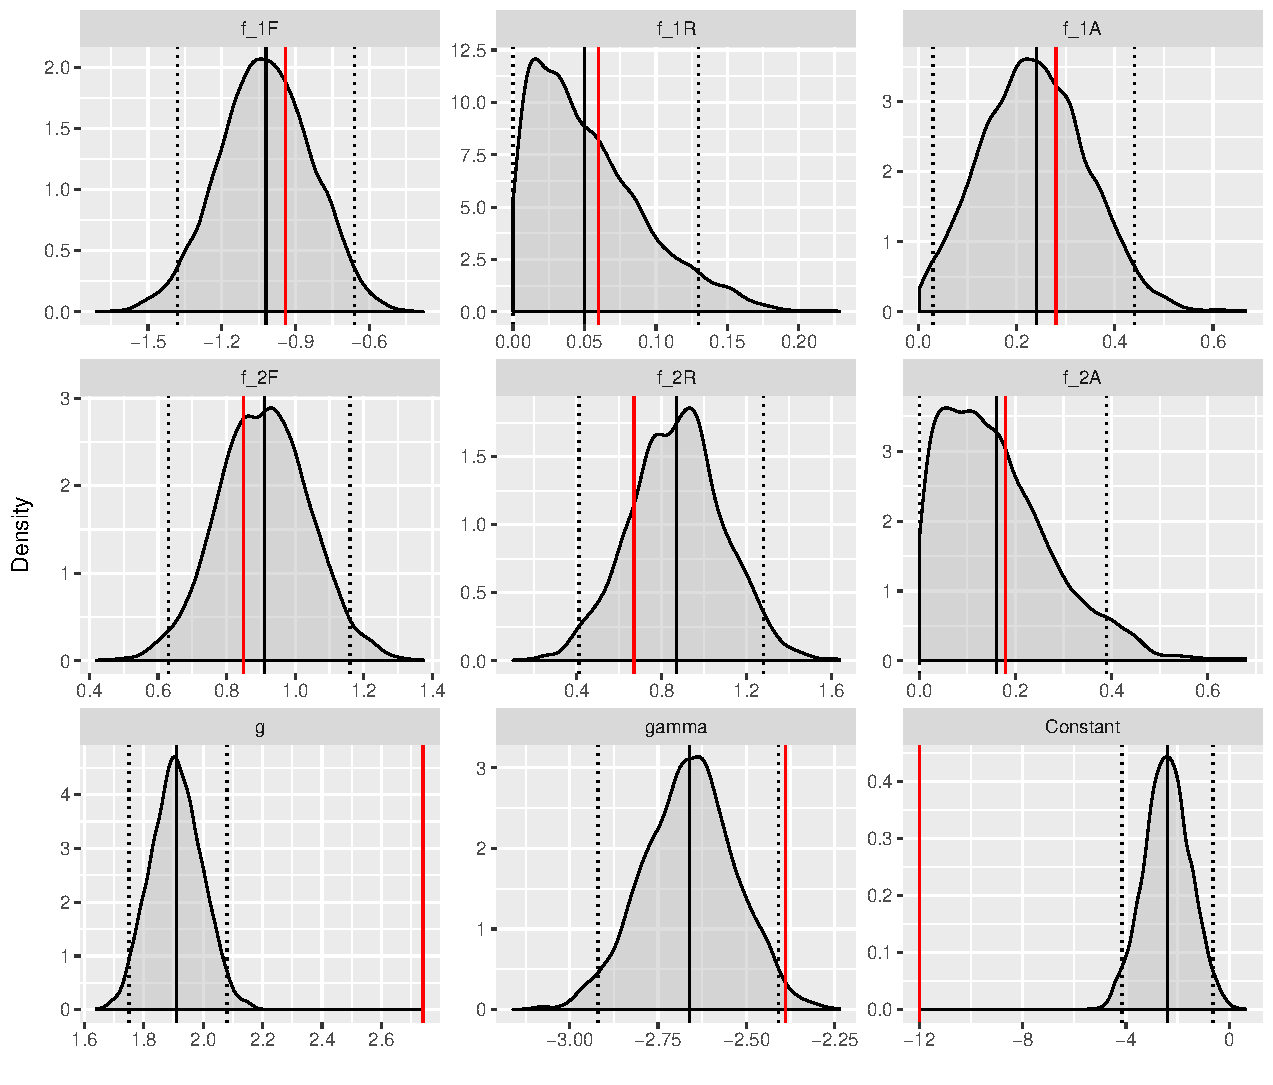
\includegraphics[width=\linewidth]{mkt4_v1f_SCOTYORK_post.pdf}
\caption{Posterior density function of elasticities w.r.t $V_{1F}$ - Market 4}
\label{fig:mkt4_v1f_SCOTYORK_post}
\caption*{Source: Own work}
\end{figure} 

% 3a
With respect to $V_{1F}$ demand, Figure \ref{fig:mkt4_v1f_SCOTYORK_post}, the only elasticity with short HDI was the $f_{1R}$, which amplitude is 0.13. For all others coefficients, the HDI range was significantly high. Detailed information of the HDI is presented in the Appendix \ref{apd:bayes_hdi}. 

% 3c
What happened in this estimation was similar to the $V_{1N}$ demand, in Market 3. The prior constraints had no effect on the likelihood and became non-informative priors since the OLS estimates already had correct signs. 

Nevertheless, two exceptions can be commented on that. It is noticeable that both $f_{1R}$ and $f_{2A}$ have an abrupt cut-off at zero, which may show that even though the mean value of OLS estimates already have correct signs, they were spreading to unfeasible values, which was cut by the prior constraint. Therefore, even though, the prior has not directly affected the mean value, it had a soft pressure in the distribution as a whole. 

% 3b
That, however, appears to be a weak pressure given the large standard deviations resulting and estimates to similar to the OLS, as explained in Market 3. Except by the $g$ and $\gamma$, all OLS estimates are lying inside the HDI interval.

\begin{figure}[H]
\centering
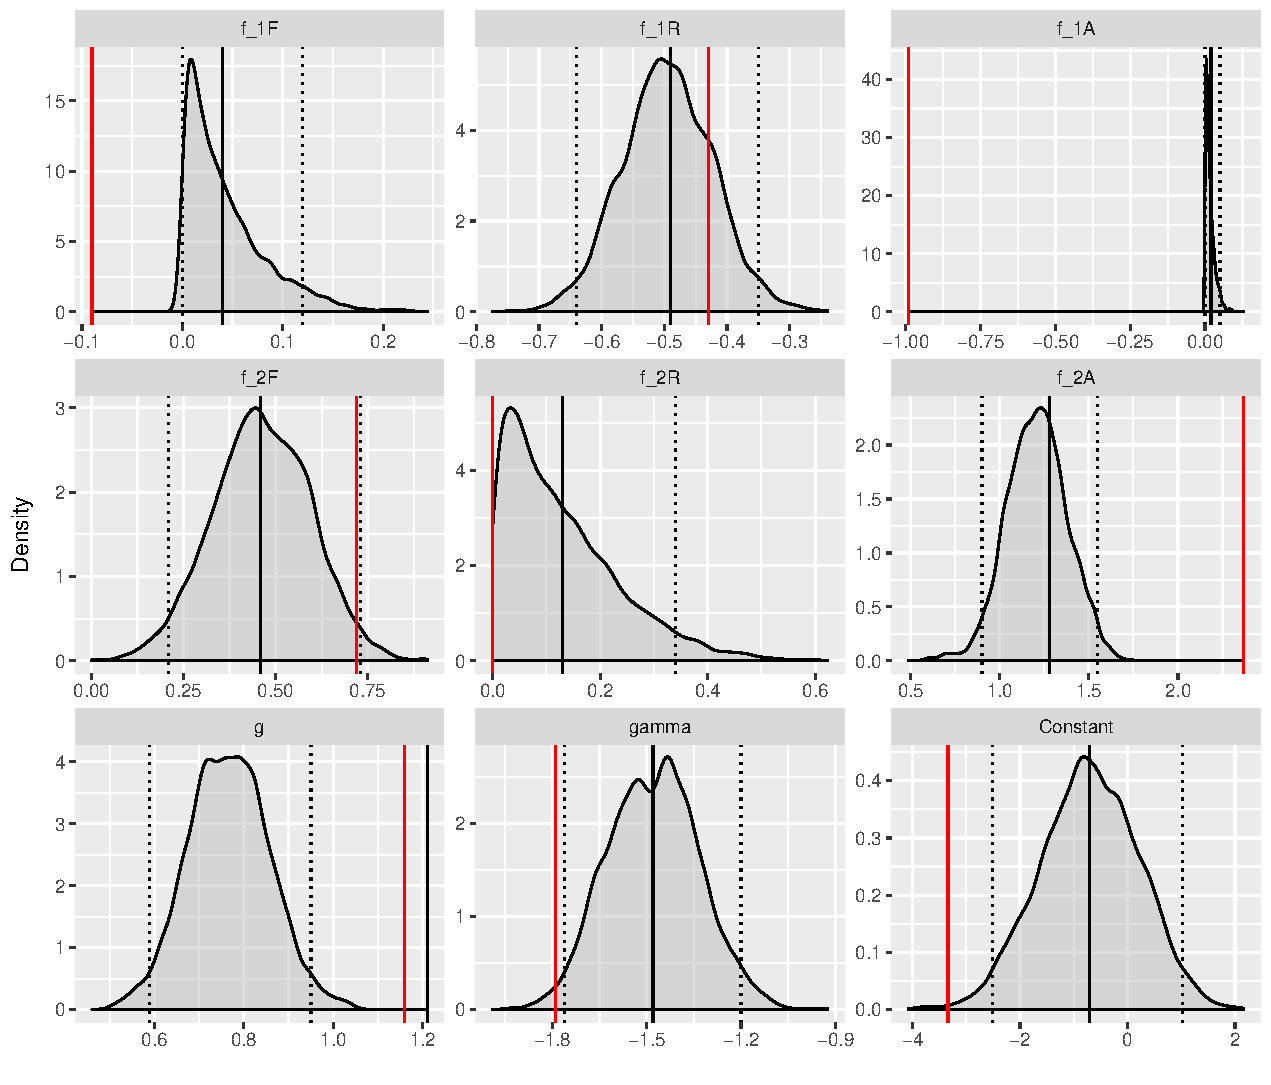
\includegraphics[width=\linewidth]{mkt4_v1r_SCOTYORK_post.pdf}
\caption{Posterior density function of elasticities w.r.t $V_{1R}$ - Market 4}
\label{fig:mkt4_v1r_SCOTYORK_post}
\caption*{Source: Own work}
\end{figure} 

% 3a
With respect to $V_{1R}$ demand, Figure \ref{fig:mkt4_v1r_SCOTYORK_post}, three elasticities presented satisfactorily small HDI: $f_{1F}$, $f_{1R}$ and $f_{1A}$, with 0.12, 0.29 and 0.05, respectively. It's noticeable that the shortest interval was the one from the sign-reversed elaticities, $f_{1F}$ and $f_{1A}$. For all others, it was above 0.30, up to 0.65 for the $f_{2R}$ elasticity. Detailed information of the HDI is presented in the Appendix \ref{apd:bayes_hdi}. 

% 3b
Even though the large HDIs, it was possible to distinguish the bayesian from OLS estimates: in addition to the sign-reversed coefficient, which should already be expected, the OLS lied out of the HDI for $f_2A$, $g$ and $\gamma$.

% 3c
Similarly to previous estimations, some distributions are skewed towards the zero constraints with sharp edges. Analogous interpretation is applicable in this regard.

\begin{figure}[H]
\centering
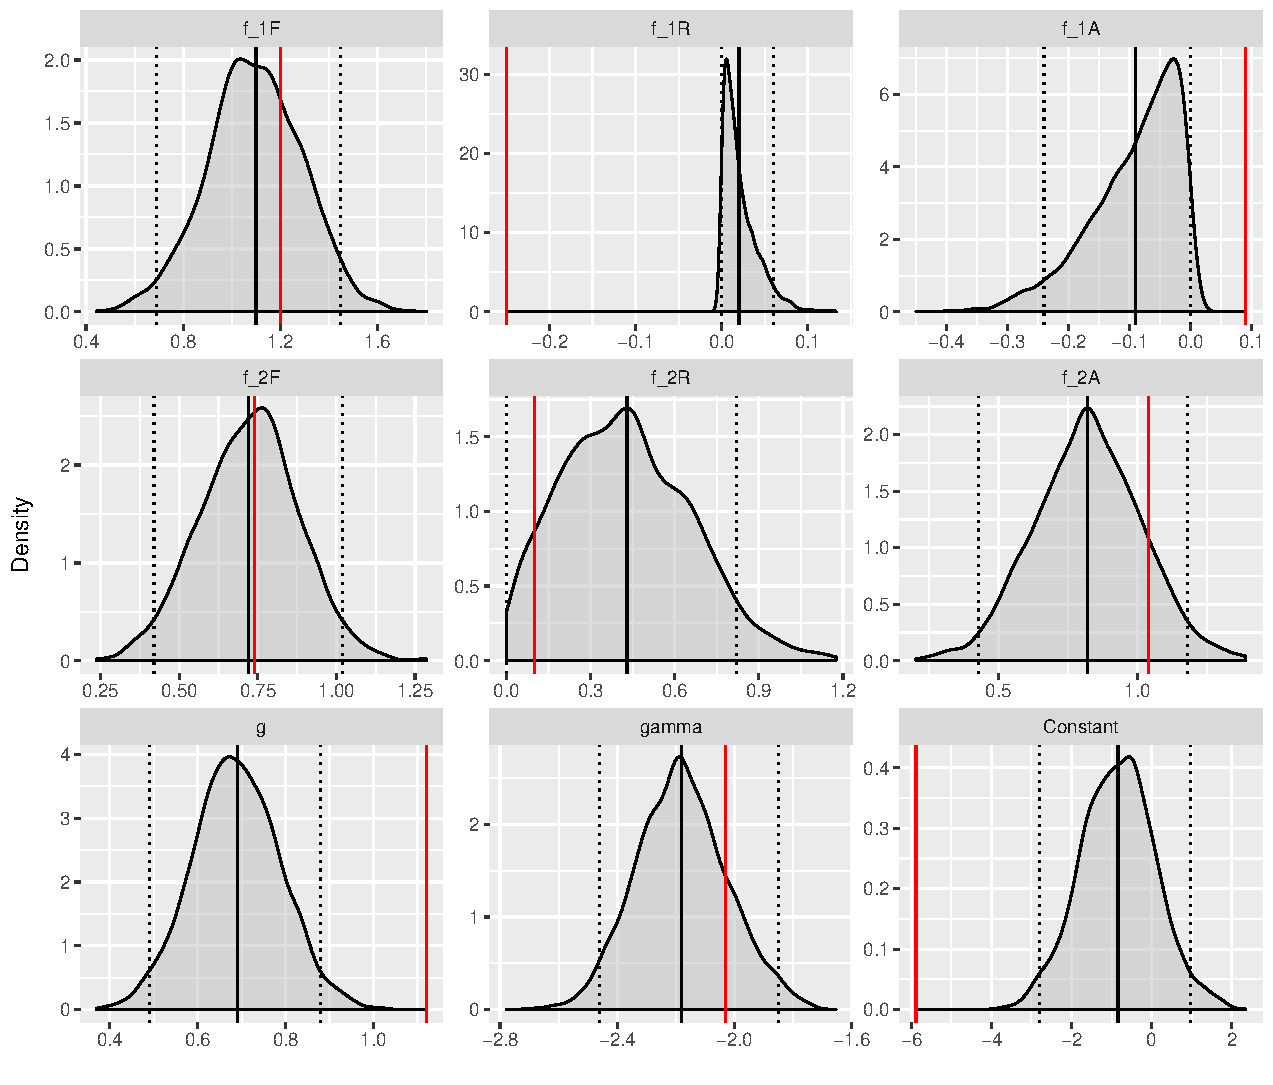
\includegraphics[width=\linewidth]{mkt4_v1a_SCOTYORK_post.pdf}
\caption{Posterior density function of elasticities w.r.t $V_{1A}$ - Market 4}
\label{fig:mkt4_v1a_SCOTYORK_post}
\caption*{Source: Own work}
\end{figure} 

% 3ac
With respect to $V_{1A}$ demand, Figure \ref{fig:mkt4_v1a_SCOTYORK_post}, only two elasticities presented short HDI's amplitude  - 0.06 for $f_{1R}$ and 0.24 for $f_{1A}$, which turn to be the constrained sign-reversed elasticities. Once again, skewness is observed and the sharp edge at zero has a similar interpretation from previous models. For all others coefficients, it was above 0.30, up to 0.82 for the $f_{2F}$. Detailed information of the HDI is presented in the Appendix \ref{apd:bayes_hdi}. 

% 3b
As it should be expected the OLS estimate lied out of the HDI for the sign-reversed elasticities. For all other elasticities, but $g$, the HDI was very large and the OLS estimates lied inside the range of 95\% probable values.

\begin{figure}[H]
\centering
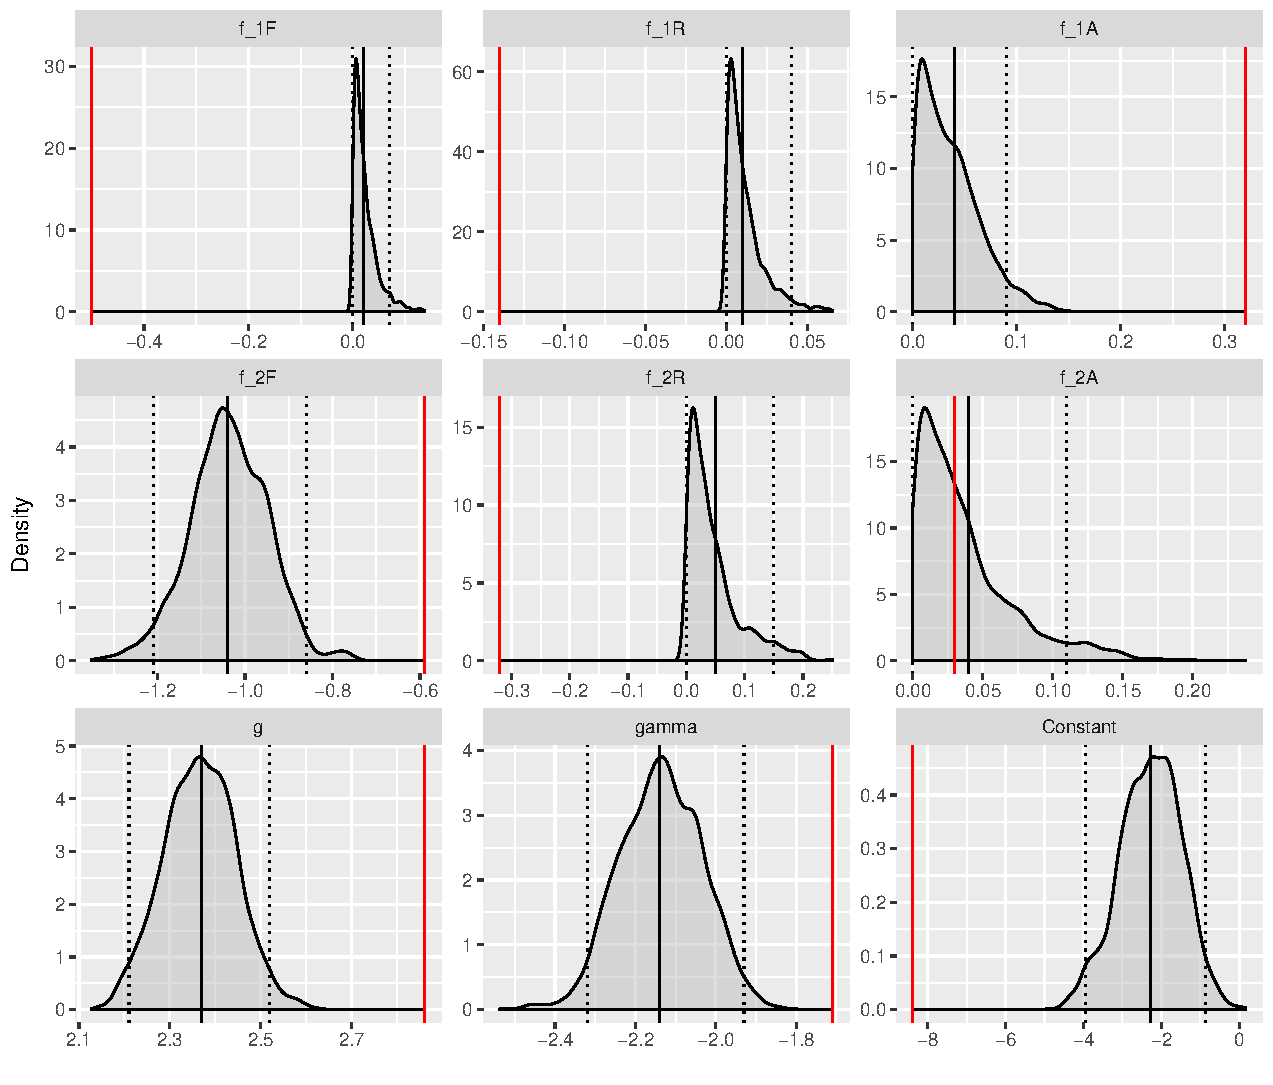
\includegraphics[width=\linewidth]{mkt4_v2f_SCOTYORK_post.pdf}
\caption{Posterior density function of elasticities w.r.t $V_{2F}$ - Market 4}
\label{fig:mkt4_v2f_SCOTYORK_post}
\caption*{Source: Own work}
\end{figure} 

% 3ac
The $V_{2F}$ model, Figure \ref{fig:mkt4_v2f_SCOTYORK_post}, was the estimation with the highest number of actual constraints. It is noticeable that the zero boundary was an actual barrier to the $f_{1F}$, $f_{1R}$, $f_{1A}$, $f_{2R}$ and $f_{2A}$ elasticities and these were the five OLS estimates wrong sign coefficients that were reverted in the Bayesian estimation.  With strong restrictions on the priors, the HDI was significantly shorter than in other estimations in this market, with five HDI ranging below 0.30. Even the ones higher 0.30 were around it, up to 0.38. Detailed information of the HDI is presented in the Appendix \ref{apd:bayes_hdi}. 

% 3b
Only the OLS elasticity of $f_{2A}$ lied inside the HDI interval, which demonstrates that squeezing the credible interval brought relevant information to the analysis.

\begin{figure}[H]
\centering
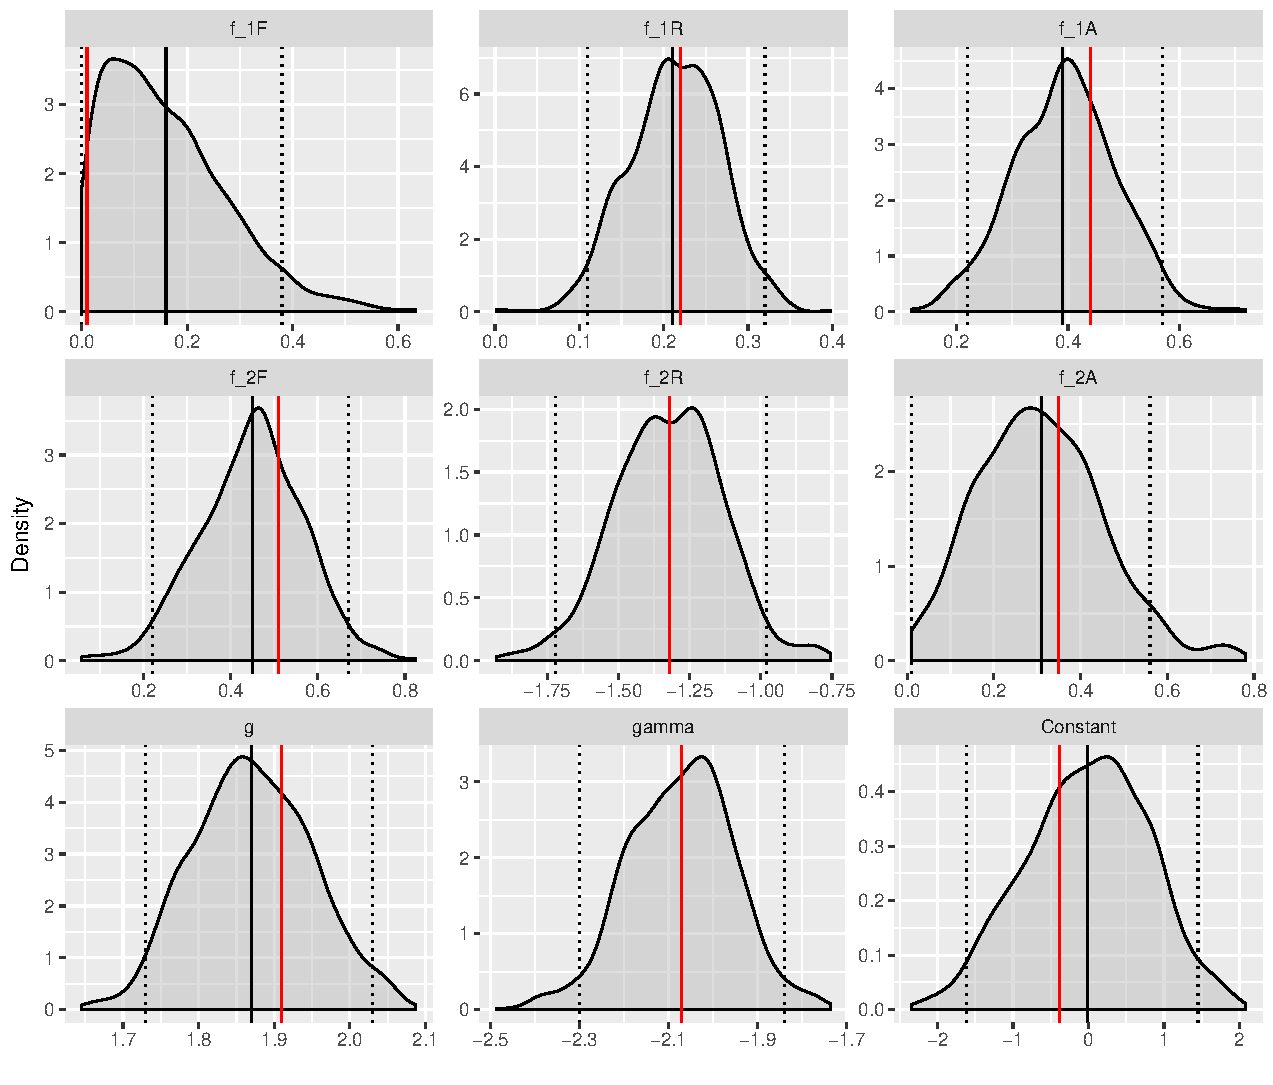
\includegraphics[width=\linewidth]{mkt4_v2r_SCOTYORK_post.pdf}
\caption{Posterior density function of elasticities w.r.t $V_{2R}$ - Market 4}
\label{fig:mkt4_v2r_SCOTYORK_post}
\caption*{Source: Own work}
\end{figure} 

% 3a
The estimation of $V_2R$ demand, Figure \ref{fig:mkt4_v2r_SCOTYORK_post}, was very similar to the $V_{1F}$ since any OLS estimates have wrong-sign. As explained before, without strong constraints, the likelihood prevailed and so the difficulty to address the correlation problems. Analogous interpretation is applied in this regard. 

The result was, once more, very large HDI, which means high uncertainty in the estimated elasticities. Only the $f_{1R}$ coefficient had HDI lower than 0.30. 

% 3b
Given that, the resultant estimates were very similar to the OLS estimates - all of them were inside the HDI. Even the $f_{2R}$ had a coincident mean.

\begin{figure}[H]
\centering
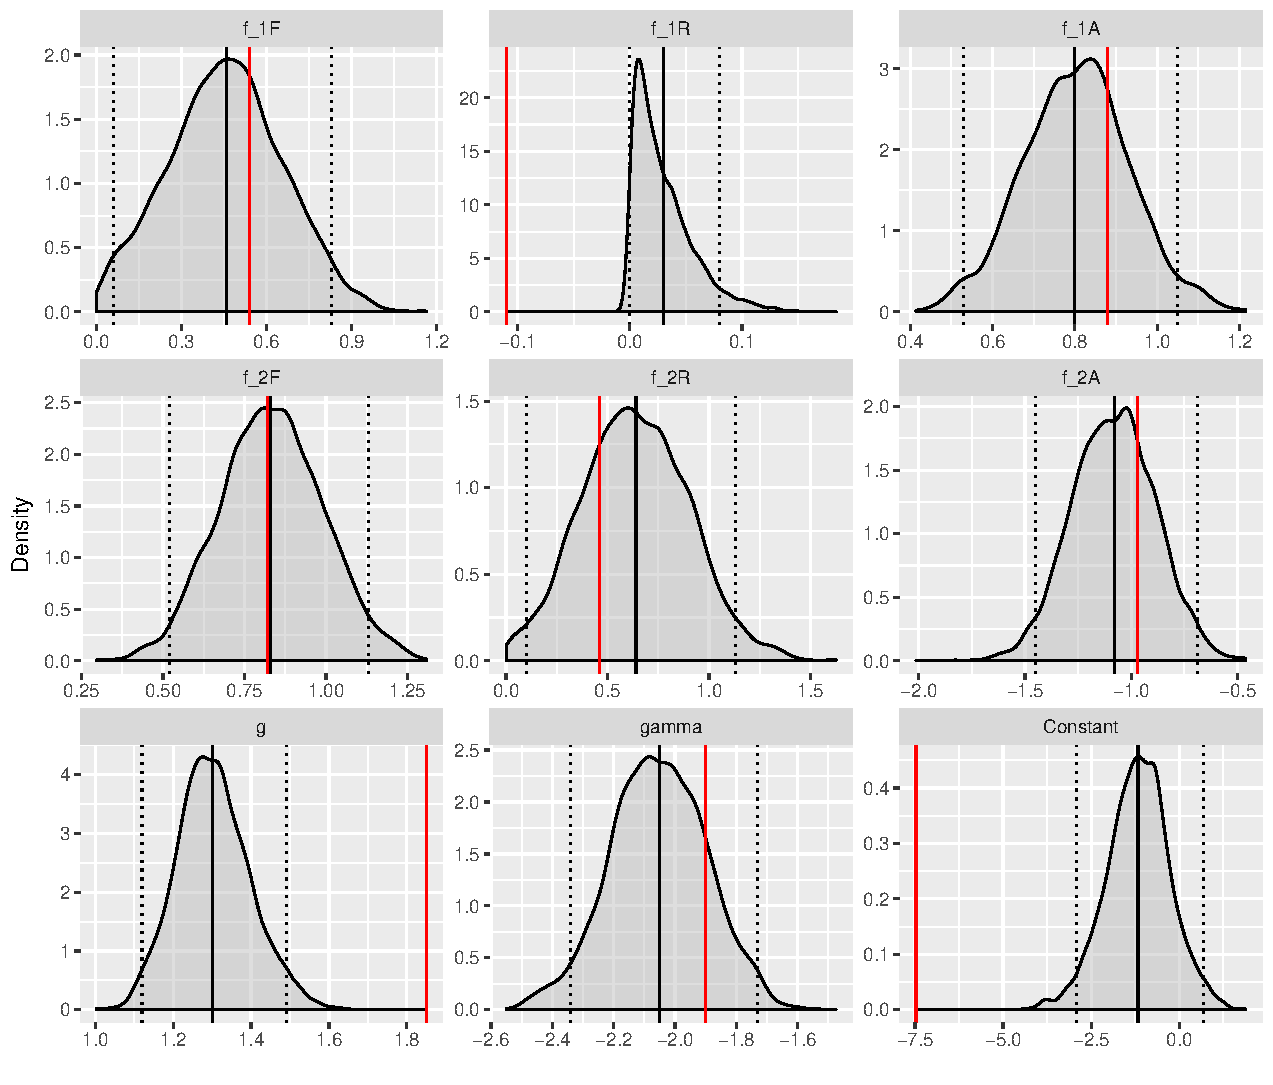
\includegraphics[width=\linewidth]{mkt4_v2a_SCOTYORK_post.pdf}
\caption{Posterior density function of elasticities w.r.t $V_{2A}$ - Market 4}
\label{fig:mkt4_v2a_SCOTYORK_post}
\caption*{Source: Own work}
\end{figure} 

% 3a
With respect to $V_2A$ demand, Figure \ref{fig:mkt4_v2a_SCOTYORK_post}, only the $f_{1R}$ elasticity suffered an actual constraint by the prior. As one may notice, it was, as usual, a wrong-sign OLS estimate reversed in the Bayesian estimation, resulting in a skewed distribution towards its boundaries. 

It appears, however, that because it is a very complex model, this was not enough to shape the other variables since all of HDI remained very large, up to 1.02. Once again, OLS lied inside the HDI, which makes one consider them as credible values, except for the $f_{1R}$, which should already be expected since it is the reversed coefficient, and the $g$ elasticities.
\\[3pt]

\textit{iv. Magnitude of estimates}

% % 0.
% Recognising that the interpretation of the estimates magnitude demands a deeper investigation of the rail market, demands support of  For that reason, the following considerations are mostly general aspects.

% 1.
Analysing the magnitude of coefficients, the most sensitive fare with regard its own price is the \textit{Standard Reduced}, with mean -1.32, followed by the \textit{Standard Advance}, \textit{Standard Full} and \textit{First Class Full}, with almost proportional effects - -1.08, -1.04 and -1.02, respectively. Smaller own elasticities were observed for the other \textit{First Class}, -0.51 and -0.09, which suggests less elastic demands. These values are considerably different from Market 3.

% 2.
Regarding to the cross elasticities, the \textit{First Class Full} fare has very small - almost null - price effects in the demand of the \textit{First Class Reduced} and \textit{Standard Full}, 0.02 and 0.05, respectively. Higher impacts, but still less than proportional occur in the demand of \textit{Standard Reduced} and \textit{Standard Advance}, 0.16 and 0.46, respectively. The \textit{First Class Advance} is surprisingly high, with 1.10, suggesting that, for first class passengers, the \textit{Advance} demand is very sensitive to changes in the \textit{Full} fare. This may sign there is a cost for passengers to plan their trips in advance.

For the \textit{First Class Reduced}, the most significant cross elasticities regarded the impact in the $V_{2R}$ demand, 0.21, all the other were very close to zero.

For the \textit{First Class Advance}, the impact in the $V_{1R}$ and $V_{2F}$ demand was also very close to zero. Higher effects were observed impacting the \textit{First Class Full} and \textit{Standard Reduced}, being of 0.24 and 0.39, respectively. The highest impact regards the \textit{Standard Advance} demand, deemed as 0.80.

Conversely, the \textit{Standard Full} have not presented such small cross elasticities. The smallest one regarding the impact in the \textit{Standard Reduced} demand, comparable to the effect in the \textit{First Class Reduced}, deemed as 0.46. The highest impact was 0.91 with regard to the \textit{First Class Full} demand.

For the \textit{Standard Reduced}, the cross elasticities with respect to the \textit{First Class Reduced} and \textit{Standard Full} demand were the smallest, 0.13 and 0.05, respectively. The biggest effect is the impact in the \textit{First Class Full}, deemes as 0.87.

The \textit{Standard Advance} had a small cross effect with respect to the \textit{First Class Full} and \textit{Standar Full}, 0.16 and 0.04, respectively. A very high impact was observed for the \textit{First Class Reduced} 1.28 - even higher than the own elasticity.

Generally, cross elasticities have ranged for very small values, close to zero, to very high ones, above 1. It was not possible to understand the interaction pattern neither even why some cross elasticities are higher than the own-elasticity.

% 3.
The GVA elasticity it worths noticing that the $g_{F} > g_{R}$ for both \textit{First} and \textit{Standard Class}, which is consistent with the fact that the percentage of business journeys is higher in \textit{Full} tickets. Additionally, the \textit{Standard Class} elasticities are higher relative to the \textit{First Class}, which may suggest that increase in productivity impacts more the mass of medium level professionals relatively to the white collar professional, that demand first class services. 

% 4.
For the GJT effects, the elasticities were considerably high: from -1.42, for the \textit{First Class Reduced} demand, to -2.66, for the \textit{First Class}. Even though there is the same GVA's reservation that states that elasticities can be expected to vary by ticket type \citep{pdfh}, it is markedly above general interval expected by PDFH - -0.7 to -1.1 \citep{pdfhv5}.
\chapter{Discussion}

\section{Conclusion}

Overall, the application of Bayesian econometrics in the estimation of rail fare elasticities have presented itself as a potential alternative to the current methods. As a proof of concept, this work has successfully worked Bayesian regressions estimating fare elasticities with coherent signs differentiating up to six fares in a market.

The primary advantage is its efficiency to estimate correct algebraic sign elasticities. All elasticities estimates were in accordance to the what is expected from the PDFH. Even for the complex Market 4, in which the \textit{First Class} tickets were broken into \textit{Full}, \textit{Reduced} and \textit{Advance}, the Bayes estimation was able to revert ten wrong signs from the SURE/OLS estimates.

The secondary advantage was the correlation being reverted to a useful feature that has helped to address the effects among correlated predictors due to the anti-correlation property of the estimates. When strong priors were defined the result was, generally, smaller standard deviations, which in turn means shorter ranges of credible values and more precise estimates.

Another advantage of Bayesian statistics regards its inherent way of interpreting probabilities, since the interpretation of posterior distribution as actual probabilities interval is much more intuitive than interpreting confidence intervals, from the sampling theory approach.

Even though the benefits, there were some issues that must be mentioned. Firstly, the occurrence of diverted transitions, which is an indicator of biased estimates. This kind of warning is supposed to raise a flag on the quality of the resulting posterior distributions. However, their occurrence may be directly related to the constraints applied in the domain of the prior distributions, which have prevented the MCMC to fully explore some regions of the parameter space. In this sense, this issue may be regarded a necessary evil to the easy application of constrained Bayes estimation in the data set.

Additionally, it was clear that the estimation has lost in quality as the models increased in complexity. This can be noticed from the difference of precision between the Markets 1 and 2, with short HDI, against Markets 3 and 4, with wider ones. Nevertheless, the later estimates can still be considered useful if one is willing to trade-off uncertainty for precision. In this study the HDI adopted regarding a range of values that represented 95\% of the probability. If the degree of certainty is reduced, for instance for an HDI of 80\%, so it will be reduced the range of credible values.

Also, in which regard the adequacy of the magnitude os estimates, even though it is recognised that it demands further development given the complexity of interactions affecting the fare elasticities, it must be pointed that some occurrences were notably out of expectations. Extremely high cross elasticities and cross elasticities bigger than the own elasticities, for instance, may deserve attention. These issues must be further investigated.

Nevertheless, acknowledging the weaknesses, the overall result was positive and with a potential practical application.

\section{Next frontiers}

As an introductory work on Bayesian econometrics applied to rail fare elasticities estimation there is plenty of further considerations that can improve the method.

In general aspects, issues that have already considered in previous studies as dynamic elasticities and the quota control for \textit{Advance} tickets were out of scope. These elements are, however, of undeniable relevance. The first one regards the differentiation between short and long-run elasticities which helps understanding how the price effects across time, which part of the price sensitiveness is immediately and which is reflected in the long-run. Some studies have reported also a cumulative effect (immediate + future) - for instance, the impact of promotions (Kopalle et al (1999) in \cite{liu2009}). The second one regards the fact that \textit{Advance} tickets are not available for all passenger, since they may sell out quickly. This supply restriction must be taken into account.

Specifically, regarding Bayesian econometrics, another possibility of should to be explored is the adoption of hierarchical models. As discussed in Chapter \ref{chp:lit-rev}, hierarchical models are being successfully applied in the retail market to estimate cross elasticities of competitors products. The rail fares have an inherent meaningful hierarchical nature that can be explored. Analogously to the retail market, in which national elasticities are decomposed to store-to-store elasticities, being able to keep regional market features, so can the broad fare elasticities be decomposed, even to route-specific elasticities. This could be a promising method to increase the ability of train operating companies in managing fares.


%-------------------------------------------------------
% POST-TEXT CONTENT

% \renewcommand{\abstractname}{Acknowledgements}
% \begin{abstract}
% \renewcommand{\thepage}{\arabic{page}}% Arabic page numbers

% This MSc was sponsored by Chevening Scholarships, the UK government’s global scholarship programme, funded by the Foreign and Commonwealth Office (FCO), in partnership with University of Leeds.

% \end{abstract}


% \section{References}
\bibliographystyle{agsm}
{\footnotesize
\bibliography{references.bib}}

\appendix

% \renewcommand\chaptername{Appendix}
\chapter{Model's Statement}
\label{apd:model_statement}



\begin{table}[!ht] \centering 
  \caption{Estimated models - Market 1} 
  \label{tbl:models_statement_mkt1} 
{\renewcommand\arraystretch{1.25}}
\begin{tabular} {ll}
\toprule
\multirow{7}{*}{$V_{2F}$} &$lnV_{2Fi} \sim Normal(\mu_i, \sigma) $ \\
                          &$\mu_i = ln a + g \cdot ln \text{GVA}_i + f_{2F} \cdot lnP_{2Fi} + f_{2R} \cdot lnP_{2Ri} + \gamma \cdot ln\text{GJT}_i$ \\
                          &$ln a \sim Normal (0,1) $\\
                          &$g \sim Normal (0,1) \quad T[0,\quad]$\\
                          &$f_{2F} \sim Normal (-0.5,0.5) \quad T[\quad,0] $\\
                          &$f_{2R} \sim Normal (0.5,0.5) \quad T[0,\quad] $\\
                          &$\gamma \sim Normal (0,1) \quad T[\quad,0] $\\
                          &$\sigma \sim uniform(0,\infty) $\\ 
\hline
\multirow{7}{*}{$V_{2R}$} &$lnV_{2Ri} \sim Normal(\mu_i, \sigma) $ \\
                          &$\mu_i = g \cdot ln \text{GVA}_i + f_{2F} \cdot lnP_{2Fi} + f_{2R} \cdot lnP_{2Ri} + \gamma \cdot ln\text{GJT}_i$ \\
                          &$ln a \sim Normal (0,1) $\\
                          &$g \sim Normal (0,1) \quad T[0,\quad]$\\
                          &$f_{2F} \sim Normal (0.5,0.5) \quad T[0,\quad] $\\
                          &$f_{2R} \sim Normal (-0.5,0.5) \quad T[\quad,0] $\\
                          &$\gamma \sim Normal (0,1) \quad T[\quad,0] $\\
                          &$\sigma \sim uniform(0,\infty) $\\ 
\bottomrule
\end{tabular}%
\caption*{Source: Own work}
\end{table} 




\begin{table}[!ht] \centering 
  \caption{Estimated models - Market 2} 
  \label{tbl:models_statement_mkt2} 
{\renewcommand\arraystretch{1.25}}
\begin{tabular} {ll}
\toprule
\multirow{7}{*}{$V_{2F}$} &$lnV_{2Fi} \sim Normal(\mu_i, \sigma) $ \\
                          &$\mu_i = g \cdot ln \text{GVA}_i + f_{2F} \cdot lnP_{2Fi} + f_{2R} \cdot lnP_{2Ri} + f_{2A} \cdot lnP_{2Ai} + \gamma \cdot ln\text{GJT}_i$ \\
                          &$g \sim Normal (0,1) \quad T[0,\quad]$\\
                          &$f_{2F} \sim Normal (-0.5,0.5) \quad T[\quad,0]$\\
                          &$f_{2R} \sim Normal (0.5,0.5) \quad T[0,\quad]$\\
                          &$f_{2A} \sim Normal (0.5,0.5) \quad T[0,\quad]$\\
                          &$\gamma \sim Normal (0,1)  \quad T[\quad,0]$\\
                          &$\sigma \sim uniform(0,\infty) $\\ 
\hline
\multirow{7}{*}{$V_{2R}$} &$lnV_{2Ri} \sim Normal(\mu_i, \sigma) $ \\
                          &$\mu_i = g \cdot ln \text{GVA}_i + f_{2F} \cdot lnP_{2Fi} + f_{2R} \cdot lnP_{2Ri} + f_{2A} \cdot lnP_{2Ai} + \gamma \cdot ln\text{GJT}_i$ \\
                          &$g \sim Normal (0,1) \quad T[0,\quad]$\\
                          &$f_{2F} \sim Normal (0.5,0.5) \quad T[0,\quad]$\\
                          &$f_{2R} \sim Normal (-0.5,0.5) \quad T[\quad,0]$\\
                          &$f_{2A} \sim Normal (0.5,0.5) \quad T[0,\quad]$\\
                          &$\gamma \sim Normal (0,1)  \quad T[\quad,0]$\\
                          &$\sigma \sim uniform(0,\infty) $\\ 
\hline
\multirow{7}{*}{$V_{2A}$} &$lnV_{2Ai} \sim Normal(\mu_i, \sigma) $ \\
                          &$\mu_i = g \cdot ln \text{GVA}_i + f_{2F} \cdot lnP_{2Fi} + f_{2R} \cdot lnP_{2Ri} + f_{2A} \cdot lnP_{2Ai} + \gamma \cdot ln\text{GJT}_i$ \\
                          &$g \sim Normal (0,1) \quad T[0,\quad]$\\
                          &$f_{2F} \sim Normal (0.5,0.5) \quad T[0,\quad]$\\
                          &$f_{2R} \sim Normal (0.5,0.5) \quad T[0,\quad]$\\
                          &$f_{2A} \sim Normal (-0.5,0.5) \quad T[\quad,0]$\\
                          &$\gamma \sim Normal (0,1)  \quad T[\quad,0]$\\
                          &$\sigma \sim uniform(0,\infty) $\\ 
\bottomrule
\end{tabular}%
\caption*{Source: Own work}
\end{table} 



\begin{table}[!ht] \centering 
  \caption{Estimated models - Market 3} 
  \label{tbl:models_statement_mkt3} 
{\renewcommand\arraystretch{1.25}}
\begin{tabular} {ll}
\toprule
\multirow{8}{*}{$V_{1N}$} &$lnV_{1Ni} \sim Normal(\mu_i, \sigma) $ \\
                          &$\mu_i = g \cdot ln \text{GVA}_i + f_{1N} \cdot lnP_{1Ni} + f_{2F} \cdot lnP_{2Fi} + f_{2R} \cdot lnP_{2Ri} + $\\
                          &$\quad \quad f_{2A} \cdot lnP_{2Ai} + \gamma \cdot ln\text{GJT}_i$ \\
                          &$g \sim Normal (0,1) \quad T[0,\quad]$\\
                          &$f_{1N} \sim Normal (-0.5,0.5) \quad T[\quad,0]$\\
                          &$f_{2F} \sim Normal (0.5,0.5) \quad T[0,\quad]$\\
                          &$f_{2R} \sim Normal (0.5,0.5) \quad T[0,\quad]$\\
                          &$f_{2A} \sim Normal (0.5,0.5) \quad T[0,\quad]$\\
                          &$\gamma \sim Normal (0,1)  \quad T[\quad,0]$\\
                          &$\sigma \sim uniform(0,\infty) $\\ 
\hline
\multirow{8}{*}{$V_{2F}$} &$lnV_{2Fi} \sim Normal(\mu_i, \sigma) $ \\
                          &$\mu_i = g \cdot ln \text{GVA}_i + f_{1N} \cdot lnP_{1Ni} + f_{2F} \cdot lnP_{2Fi} + f_{2R} \cdot lnP_{2Ri} + $\\
                          &$\quad \quad f_{2A} \cdot lnP_{2Ai} + \gamma \cdot ln\text{GJT}_i$ \\
                          &$g \sim Normal (0,1) \quad T[0,\quad]$\\
                          &$f_{1N} \sim Normal (0.5,0.5) \quad T[0,\quad]$\\
                          &$f_{2F} \sim Normal (-0.5,0.5) \quad T[\quad,0]$\\
                          &$f_{2R} \sim Normal (0.5,0.5) \quad T[0,\quad]$\\
                          &$f_{2A} \sim Normal (0.5,0.5) \quad T[0,\quad]$\\
                          &$\gamma \sim Normal (0,1)  \quad T[\quad,0]$\\
                          &$\sigma \sim uniform(0,\infty) $\\ 
\hline
\multirow{8}{*}{$V_{2R}$} &$lnV_{2Ri} \sim Normal(\mu_i, \sigma) $ \\
                          &$\mu_i = g \cdot ln \text{GVA}_i + f_{1N} \cdot lnP_{1Ni} + f_{2F} \cdot lnP_{2Fi} + f_{2R} \cdot lnP_{2Ri} + $\\
                          &$\quad \quad f_{2A} \cdot lnP_{2Ai} + \gamma \cdot ln\text{GJT}_i$ \\
                          &$g \sim Normal (0,1) \quad T[0,\quad]$\\
                          &$f_{1N} \sim Normal (0.5,0.5) \quad T[0,\quad]$\\
                          &$f_{2F} \sim Normal (0.5,0.5) \quad T[0,\quad]$\\
                          &$f_{2R} \sim Normal (-0.5,0.5) \quad T[\quad,0]$\\
                          &$f_{2A} \sim Normal (0.5,0.5) \quad T[0,\quad]$\\
                          &$\gamma \sim Normal (0,1)  \quad T[\quad,0]$\\
                          &$\sigma \sim uniform(0,\infty) $\\ 
\hline
\multirow{8}{*}{$V_{2A}$} &$lnV_{2Ai} \sim Normal(\mu_i, \sigma) $ \\
                          &$\mu_i = g \cdot ln \text{GVA}_i + f_{1N} \cdot lnP_{1Ni} + f_{2F} \cdot lnP_{2Fi} + f_{2R} \cdot lnP_{2Ri} + $\\
                          &$\quad \quad f_{2A} \cdot lnP_{2Ai} + \gamma \cdot ln\text{GJT}_i$ \\
                          &$g \sim Normal (0,1) \quad T[0,\quad]$\\
                          &$f_{1N} \sim Normal (0.5,0.5) \quad T[0,\quad]$\\
                          &$f_{2F} \sim Normal (0.5,0.5) \quad T[0,\quad]$\\
                          &$f_{2R} \sim Normal (0.5,0.5) \quad T[0,\quad]$\\
                          &$f_{2A} \sim Normal (-0.5,0.5) \quad T[\quad,0]$\\
                          &$\gamma \sim Normal (0,1)  \quad T[\quad,0]$\\
                          &$\sigma \sim uniform(0,\infty) $\\ 
\bottomrule
\end{tabular}%
\caption*{Source: Own work}
\end{table} 



\begin{table}[!ht] \centering 
  \caption{Estimated models - Market 4 [Part 1/2]} 
  \label{tbl:models_statement_mkt4_1} 
{\renewcommand\arraystretch{1.25}}
\begin{tabular} {ll}
\toprule
\multirow{12}{*}{$V_{1F}$}&$lnV_{1Fi} \sim Normal(\mu_i, \sigma) $ \\
                          &$\mu_i = g \cdot ln \text{GVA}_i + f_{1F} \cdot lnP_{1Fi} + f_{1R} \cdot lnP_{1Ri} + f_{1A} \cdot lnP_{1Ai} +$\\
                          &$\quad \quad f_{2F} \cdot lnP_{2Fi} + f_{2R} \cdot lnP_{2Ri} + f_{2A} \cdot lnP_{2Ai} + \gamma \cdot ln\text{GJT}_i$ \\
                          &$g \sim Normal (0,1) \quad T[0,\quad]$\\
                          &$f_{1F} \sim Normal (-0.5,0.5) \quad T[\quad,0]$\\
                          &$f_{1R} \sim Normal (0.5,0.5) \quad T[0,\quad]$\\
                          &$f_{1A} \sim Normal (0.5,0.5) \quad T[0,\quad]$\\
                          &$f_{2F} \sim Normal (0.5,0.5) \quad T[0,\quad]$\\
                          &$f_{2R} \sim Normal (0.5,0.5) \quad T[0,\quad]$\\
                          &$f_{2A} \sim Normal (0.5,0.5) \quad T[0,\quad]$\\
                          &$\gamma \sim Normal (0,1)  \quad T[\quad,0]$\\
                          &$\sigma \sim uniform(0,\infty) $\\ 
\hline
\multirow{12}{*}{$V_{1R}$}&$lnV_{1Ri} \sim Normal(\mu_i, \sigma) $ \\
                          &$\mu_i = g \cdot ln \text{GVA}_i + f_{1F} \cdot lnP_{1Fi} + f_{1R} \cdot lnP_{1Ri} + f_{1A} \cdot lnP_{1Ai} +$\\
                          &$\quad \quad f_{2F} \cdot lnP_{2Fi} + f_{2R} \cdot lnP_{2Ri} + f_{2A} \cdot lnP_{2Ai} + \gamma \cdot ln\text{GJT}_i$ \\
                          &$g \sim Normal (0,1) \quad T[0,\quad]$\\
                          &$f_{1F} \sim Normal (0.5,0.5) \quad T[0,\quad]$\\
                          &$f_{1R} \sim Normal (-0.5,0.5) \quad T[\quad,0]$\\
                          &$f_{1A} \sim Normal (0.5,0.5) \quad T[0,\quad]$\\
                          &$f_{2F} \sim Normal (0.5,0.5) \quad T[0,\quad]$\\
                          &$f_{2R} \sim Normal (0.5,0.5) \quad T[0,\quad]$\\
                          &$f_{2A} \sim Normal (0.5,0.5) \quad T[0,\quad]$\\
                          &$\gamma \sim Normal (0,1)  \quad T[\quad,0]$\\
                          &$\sigma \sim uniform(0,\infty) $\\ 
\hline
\multirow{12}{*}{$V_{1A}$}&$lnV_{1Ai} \sim Normal(\mu_i, \sigma) $ \\
                          &$\mu_i = g \cdot ln \text{GVA}_i + f_{1F} \cdot lnP_{1Fi} + f_{1R} \cdot lnP_{1Ri} + f_{1A} \cdot lnP_{1Ai} +$\\
                          &$\quad \quad f_{2F} \cdot lnP_{2Fi} + f_{2R} \cdot lnP_{2Ri} + f_{2A} \cdot lnP_{2Ai} + \gamma \cdot ln\text{GJT}_i$ \\
                          &$g \sim Normal (0,1) \quad T[0,\quad]$\\
                          &$f_{1F} \sim Normal (0.5,0.5) \quad T[0,\quad]$\\
                          &$f_{1R} \sim Normal (0.5,0.5) \quad T[0,\quad]$\\
                          &$f_{1A} \sim Normal (-0.5,0.5) \quad T[\quad,0]$\\
                          &$f_{2F} \sim Normal (0.5,0.5) \quad T[0,\quad]$\\
                          &$f_{2R} \sim Normal (0.5,0.5) \quad T[0,\quad]$\\
                          &$f_{2A} \sim Normal (0.5,0.5) \quad T[0,\quad]$\\
                          &$\gamma \sim Normal (0,1)  \quad T[\quad,0]$\\
                          &$\sigma \sim uniform(0,\infty) $\\ 
\bottomrule
\end{tabular}%
\caption*{Source: Own work}
\end{table} 



\begin{table}[!ht] \centering 
  \caption{Estimated models - Market 4 [Part 2/2]} 
  \label{tbl:models_statement_mkt4_2} 
{\renewcommand\arraystretch{1.25}}
\begin{tabular} {ll}
\toprule
\multirow{12}{*}{$V_{2F}$} &$lnV_{2Fi} \sim Normal(\mu_i, \sigma) $ \\
                          &$\mu_i = g \cdot ln \text{GVA}_i + f_{1F} \cdot lnP_{1Fi} + f_{1R} \cdot lnP_{1Ri} + f_{1A} \cdot lnP_{1Ai} +$\\
                          &$\quad \quad f_{2F} \cdot lnP_{2Fi} + f_{2R} \cdot lnP_{2Ri} + f_{2A} \cdot lnP_{2Ai} + \gamma \cdot ln\text{GJT}_i$ \\
                          &$g \sim Normal (0,1) \quad T[0,\quad]$\\
                          &$f_{1F} \sim Normal (0.5,0.5) \quad T[0,\quad]$\\
                          &$f_{1R} \sim Normal (0.5,0.5) \quad T[0,\quad]$\\
                          &$f_{1A} \sim Normal (0.5,0.5) \quad T[0,\quad]$\\
                          &$f_{2F} \sim Normal (-0.5,0.5) \quad T[\quad,0]$\\
                          &$f_{2R} \sim Normal (0.5,0.5) \quad T[0,\quad]$\\
                          &$f_{2A} \sim Normal (0.5,0.5) \quad T[0,\quad]$\\
                          &$\gamma \sim Normal (0,1)  \quad T[\quad,0]$\\
                          &$\sigma \sim uniform(0,\infty) $\\ 
\hline
\multirow{12}{*}{$V_{2R}$} &$lnV_{2Ri} \sim Normal(\mu_i, \sigma) $ \\
                          &$\mu_i = g \cdot ln \text{GVA}_i + f_{1F} \cdot lnP_{1Fi} + f_{1R} \cdot lnP_{1Ri} + f_{1A} \cdot lnP_{1Ai} +$\\
                          &$\quad \quad f_{2F} \cdot lnP_{2Fi} + f_{2R} \cdot lnP_{2Ri} + f_{2A} \cdot lnP_{2Ai} + \gamma \cdot ln\text{GJT}_i$ \\
                          &$g \sim Normal (0,1) \quad T[0,\quad]$\\
                          &$f_{1F} \sim Normal (0.5,0.5) \quad T[0,\quad]$\\
                          &$f_{1R} \sim Normal (0.5,0.5) \quad T[0,\quad]$\\
                          &$f_{1A} \sim Normal (0.5,0.5) \quad T[0,\quad]$\\
                          &$f_{2F} \sim Normal (0.5,0.5) \quad T[0,\quad]$\\
                          &$f_{2R} \sim Normal (-0.5,0.5) \quad T[\quad,0]$\\
                          &$f_{2A} \sim Normal (0.5,0.5) \quad T[0,\quad]$\\
                          &$\gamma \sim Normal (0,1)  \quad T[\quad,0]$\\
                          &$\sigma \sim uniform(0,\infty) $\\ 
\hline
\multirow{12}{*}{$V_{2A}$} &$lnV_{2Ai} \sim Normal(\mu_i, \sigma) $ \\
                          &$\mu_i = g \cdot ln \text{GVA}_i + f_{1F} \cdot lnP_{1Fi} + f_{1R} \cdot lnP_{1Ri} + f_{1A} \cdot lnP_{1Ai} +$\\
                          &$\quad \quad f_{2F} \cdot lnP_{2Fi} + f_{2R} \cdot lnP_{2Ri} + f_{2A} \cdot lnP_{2Ai} + \gamma \cdot ln\text{GJT}_i$ \\
                          &$g \sim Normal (0,1) \quad T[0,\quad]$\\
                          &$f_{1F} \sim Normal (0.5,0.5) \quad T[0,\quad]$\\
                          &$f_{1R} \sim Normal (0.5,0.5) \quad T[0,\quad]$\\
                          &$f_{1A} \sim Normal (0.5,0.5) \quad T[0,\quad]$\\
                          &$f_{2F} \sim Normal (0.5,0.5) \quad T[0,\quad]$\\
                          &$f_{2R} \sim Normal (0.5,0.5) \quad T[0,\quad]$\\
                          &$f_{2A} \sim Normal (-0.5,0.5) \quad T[\quad,0]$\\
                          &$\gamma \sim Normal (0,1)  \quad T[\quad,0]$\\
                          &$\sigma \sim uniform(0,\infty) $\\ 
\bottomrule
\end{tabular}%
\caption*{Source: Own work}
\end{table} 





% 
\renewcommand\chaptername{Appendix}
\chapter{SURE Estimation}
\label{apd:sure}


% \begin{landscape}
% 
\begin{table}[!ht] \centering 
  \caption{OLS Estimates - [Part 1/2]} 
  \label{tbl:ols} 
{\renewcommand\arraystretch{1.25}}
\begin{tabular} {c c ccccccc cc}
\toprule
\multirow{2}{*}{Market} & Estimated  & \multicolumn{7}{c}{Fare Elasticities}                                   & \multicolumn{2}{c}{Other Elasticties} \\
						& Demand     & $f_{1F}$ & $f_{1R}$ & $f_{1A}$ & $f_{1N}$ & $f_{2F}$ & $f_{2R}$ & $f_{2A}$ & $g$ & $\gamma$ \\ 
\hline
\multirow{4}{*}{1}      & \multirow{2}{*}{$V_{2F}$}   & & & & & & & & & \\
													  & & & & & & & & & \\
						\cdashline{2-11}
						& \multirow{2}{*}{$V_{2R}$}   & & & & & & & & & \\
													  & & & & & & & & & \\
\hline
\multirow{6}{*}{2}      & \multirow{2}{*}{$V_{2F}$}   & & & & & & & & & \\
													  & & & & & & & & & \\
						& \multirow{2}{*}{$V_{2R}$}   & & & & & & & & & \\
													  & & & & & & & & & \\
						& \multirow{2}{*}{$V_{2A}$}   & & & & & & & & & \\
													  & & & & & & & & & \\
\hline
\multirow{8}{*}{3}      & \multirow{2}{*}{$V_{1N}$}   & & & & & & & & & \\
													  & & & & & & & & & \\
						& \multirow{2}{*}{$V_{2F}$}   & & & & & & & & & \\
													  & & & & & & & & & \\
						& \multirow{2}{*}{$V_{2R}$}   & & & & & & & & & \\
													  & & & & & & & & & \\
						& \multirow{2}{*}{$V_{2A}$}   & & & & & & & & & \\
													  & & & & & & & & & \\
\bottomrule
\end{tabular}%
\caption*{Source: Own work}
\end{table} 

% \end{landscape}

% \begin{landscape}
% 
\begin{table}[!ht] \centering 
  \caption{OLS Estimates - [Part 2/2]} 
  \label{tbl:ols} 
{\renewcommand\arraystretch{1.25}}
\begin{tabular} {c c cccccccc cc}
\toprule
\multirow{2}{*}{Market} & Estimated  & \multicolumn{7}{c}{Fare Elasticities}                                   & \multicolumn{2}{c}{Other Elasticties} \\
						& Demand     & Intcp & $f_{1F}$ & $f_{1R}$ & $f_{1A}$ & $f_{1N}$ & $f_{2F}$ & $f_{2R}$ & $f_{2A}$ & $g$ & $\gamma$ \\ 
\hline
\multirow{12}{*}{4}      & \multirow{2}{*}{$V_{1F}$}  &$3.56^{***}$ &$-1.58^{***}$&$-0.35^{***}$& $-0.37^{***}$& - & $-0.16^{***}$& $3.38^{***}$& $0.23^{***}$& $1.37^{***}$& $-2.64^{***}$\\
						&							  &$(0.62)$&$(0.04)$&$(0.01)$ &$(0.03)$ & - & $(0.04)$ &$(0.07)$ &$(0.05)$ &$(0.06)$ &$(0.04)$ \\
						& \multirow{2}{*}{$V_{1R}$}   & & & & & & & & & \\
													  & & & & & & & & & \\
						& \multirow{2}{*}{$V_{1A}$}   & & & & & & & & & \\
													  & & & & & & & & & \\
						& \multirow{2}{*}{$V_{2F}$}   & & & & & & & & & \\
													  & & & & & & & & & \\
						& \multirow{2}{*}{$V_{2R}$}   & & & & & & & & & \\
													  & & & & & & & & & \\
						& \multirow{2}{*}{$V_{2A}$}   & & & & & & & & & \\
													  & & & & & & & & & \\
\bottomrule
\end{tabular}%
\caption*{Source: Own work}
\end{table} 

% \end{landscape}


\begin{table}[!htbp] \centering 
  \caption{OLS Estimates - Market 1} 
  \label{} 
\begin{tabular}{@{\extracolsep{5pt}}lcc} 
\toprule 
 & \multicolumn{2}{c}{\textit{Dependent variable:}} \\ 
\cline{2-3} 
\\[-1.8ex] & $ln \; V_{2F}$ & $ln \; V_{2R}$ \\ 
\hline \\[-1.8ex] 
 $f_{2F}$ & $-$1.281$^{***}$ & 0.811$^{***}$ \\ 
  & (0.048) & (0.049) \\ 
  & & \\ 
 $f_{2R}$ & 0.173$^{***}$ & $-$0.895$^{***}$ \\ 
  & (0.049) & (0.050) \\ 
  & & \\ 
 $g$ & 0.493$^{***}$ & $-$0.517$^{***}$ \\ 
  & (0.066) & (0.068) \\ 
  & & \\ 
 $\gamma$ & $-$0.976$^{***}$ & $-$1.062$^{***}$ \\ 
  & (0.045) & (0.046) \\ 
  & & \\ 
 Constant & 9.138$^{***}$ & 17.582$^{***}$ \\ 
  & (0.710) & (0.730) \\ 
  & & \\ 
\hline 
\hline \\[-1.8ex] 
\textit{Note:}  & \multicolumn{2}{r}{$^{*}$p$<$0.1; $^{**}$p$<$0.05; $^{***}$p$<$0.01} \\
\bottomrule 
\end{tabular}
\caption*{Source: Own work} 
\end{table} 

\begin{table}[!htbp] \centering 
  \caption{OLS Estimates - Market 2} 
  \label{} 
\begin{tabular}{@{\extracolsep{5pt}}lccc} 
\toprule 
 & \multicolumn{3}{c}{\textit{Dependent variable:}} \\ 
\cline{2-4} 
\\[-1.8ex] & $ln \; V_{2F}$ & $ln \; V_{2R}$ & $ln \; V_{2A}$ \\ 
\hline \\[-1.8ex] 
 $f_{2F}$ & $-$1.241$^{***}$ & 0.032 & $-$0.183$^{*}$ \\ 
  & (0.063) & (0.059) & (0.097) \\ 
  & & & \\ 
 $f_{2R}$ & $-$0.056 & $-$0.597$^{***}$ & 1.034$^{***}$ \\ 
  & (0.084) & (0.079) & (0.130) \\ 
  & & & \\ 
 $f_{2A}$ & 0.152$^{***}$ & $-$0.105$^{***}$ & $-$0.467$^{***}$ \\ 
  & (0.039) & (0.037) & (0.061) \\ 
  & & & \\ 
 $g$ & 1.749$^{***}$ & 0.388$^{***}$ & 0.661$^{***}$ \\ 
  & (0.108) & (0.102) & (0.166) \\ 
  & & & \\ 
 $\gamma$ & $-$1.231$^{***}$ & $-$1.213$^{***}$ & 0.334$^{***}$ \\ 
  & (0.066) & (0.062) & (0.102) \\ 
  & & & \\ 
 Constant & $-$1.094 & 11.716$^{***}$ & $-$5.528$^{***}$ \\ 
  & (1.153) & (1.086) & (1.772) \\ 
  & & & \\ 
\hline 
\hline \\[-1.8ex] 
\textit{Note:}  & \multicolumn{3}{r}{$^{*}$p$<$0.1; $^{**}$p$<$0.05; $^{***}$p$<$0.01} \\ 
\bottomrule 
\end{tabular}
\caption*{Source: Own work} 
\end{table} 

\begin{table}[!htbp] \centering 
  \caption{OLS Estimates - Market 3} 
  \label{} 
\begin{tabular}{@{\extracolsep{5pt}}lcccc} 
\toprule 
 & \multicolumn{4}{c}{\textit{Dependent variable:}} \\ 
\cline{2-5} 
\\[-1.8ex] & $ln \; V_{1N}$ & $ln \; V_{2F}$ & $ln \; V_{2R}$ & $ln \; V_{2A}$ \\ 
\hline \\[-1.8ex] 
$f_{1N}$ & $-$1.516$^{***}$ & 0.068$^{***}$ & $-$0.316$^{***}$ & $-$0.670$^{***}$ \\ 
  & (0.013) & (0.010) & (0.010) & (0.015) \\ 
  & & & & \\ 
 $f_{2F}$ & 0.212$^{***}$ & $-$1.302$^{***}$ & $-$0.224$^{***}$ & 0.485$^{***}$ \\ 
  & (0.020) & (0.017) & (0.016) & (0.024) \\ 
  & & & & \\ 
 $f_{2R}$ & 2.855$^{***}$ & 0.524$^{***}$ & 0.116$^{***}$ & 3.166$^{***}$ \\ 
  & (0.032) & (0.027) & (0.025) & (0.038) \\ 
  & & & & \\ 
 $f_{2A}$ & 0.216$^{***}$ & 0.313$^{***}$ & $-$0.054$^{***}$ & $-$0.866$^{***}$ \\ 
  & (0.020) & (0.016) & (0.015) & (0.023) \\ 
  & & & & \\ 
 $g$ & 0.885$^{***}$ & 1.426$^{***}$ & 0.558$^{***}$ & 0.919$^{***}$ \\ 
  & (0.034) & (0.028) & (0.026) & (0.040) \\ 
  & & & & \\ 
 $\gamma$ & $-$2.755$^{***}$ & $-$1.910$^{***}$ & $-$1.411$^{***}$ & $-$2.144$^{***}$ \\ 
  & (0.023) & (0.019) & (0.018) & (0.027) \\ 
  & & & & \\ 
 Constant & 6.143$^{***}$ & 3.934$^{***}$ & 11.331$^{***}$ & 1.189$^{***}$ \\ 
  & (0.360) & (0.299) & (0.280) & (0.427) \\ 
  & & & & \\  
\hline 
\hline \\[-1.8ex] 
\textit{Note:}  & & \multicolumn{3}{r}{$^{*}$p$<$0.1; $^{**}$p$<$0.05; $^{***}$p$<$0.01} \\ 
\bottomrule 
\end{tabular}
\caption*{Source: Own work} 
\end{table} 


\begin{table}[!htbp] \centering 
  \caption{OLS Estimates - Market 3 (Scotland - Yorkshire)} 
  \label{} 
\begin{tabular}{@{\extracolsep{5pt}}lcccc} 
\toprule 
 & \multicolumn{4}{c}{\textit{Dependent variable:}} \\ 
\cline{2-5} 
\\[-1.8ex] & $ln \; V_{1N}$ & $ln \; V_{2F}$ & $ln \; V_{2R}$ & $ln \; V_{2A}$ \\ 
\hline \\[-1.8ex] 
 $f_{1N}$ & $-$0.839$^{***}$ & $-$0.428$^{***}$ & $-$0.437$^{***}$ & $-$0.502$^{***}$ \\ 
  & (0.061) & (0.050) & (0.047) & (0.072) \\ 
  & & & & \\ 
 $f_{2F}$ & 1.031$^{***}$ & $-$1.122$^{***}$ & 0.232$^{***}$ & 1.074$^{***}$ \\ 
  & (0.088) & (0.072) & (0.068) & (0.104) \\ 
  & & & & \\ 
 $f_{2R}$ & 1.794$^{***}$ & $-$0.036 & 0.340$^{***}$ & 2.279$^{***}$ \\ 
  & (0.110) & (0.089) & (0.085) & (0.130) \\ 
  & & & & \\ 
 $f_{2A}$ & 0.430$^{***}$ & 0.327$^{***}$ & 0.146$^{***}$ & $-$0.387$^{***}$ \\ 
  & (0.063) & (0.051) & (0.049) & (0.074) \\ 
  & & & & \\ 
 $g$ & 1.503$^{***}$ & 1.660$^{***}$ & 0.804$^{***}$ & 1.541$^{***}$ \\ 
  & (0.114) & (0.093) & (0.088) & (0.135) \\ 
  & & & & \\ 
 $\gamma$ & $-$3.298$^{***}$ & $-$1.603$^{***}$ & $-$2.311$^{***}$ & $-$2.007$^{***}$ \\ 
  & (0.082) & (0.066) & (0.063) & (0.096) \\ 
  & & & & \\ 
 Constant & 0.619 & 2.851$^{***}$ & 11.662$^{***}$ & $-$6.722$^{***}$ \\ 
  & (1.227) & (0.999) & (0.945) & (1.448) \\ 
  & & & & \\ 
\hline 
\hline \\[-1.8ex] 
\textit{Note:}  & & \multicolumn{3}{r}{$^{*}$p$<$0.1; $^{**}$p$<$0.05; $^{***}$p$<$0.01} \\ 
\bottomrule 
\end{tabular}
\caption*{Source: Own work} 
\end{table} 

\begin{table}[!htbp] \centering 
  \caption{OLS Estimates - Market 4} 
  \label{} 
\begin{tabular}{@{\extracolsep{5pt}}lcccccc} 
\toprule 
 & \multicolumn{6}{c}{\textit{Dependent variable:}} \\ 
\cline{2-7} 
\\[-1.8ex] & $ln \; V_{1F}$ & $ln \; V_{1R}$ & $ln \; V_{1A}$ & $ln \; V_{2F}$ & $ln \; V_{2R}$ & $ln \; V_{2A}$ \\ 
\hline \\[-1.8ex] 
  $f_{1F}$ & $-$1.584$^{***}$ & $-$0.174$^{***}$ & $-$0.013 & $-$0.248$^{***}$ & $-$0.289$^{***}$ & 0.106$^{**}$ \\ 
  & (0.040) & (0.047) & (0.051) & (0.035) & (0.032) & (0.043) \\ 
  & & & & & & \\ 
 $f_{1R}$ & $-$0.346$^{***}$ & $-$0.257$^{***}$ & $-$0.292$^{***}$ & $-$0.136$^{***}$ & $-$0.137$^{***}$ & $-$0.113$^{***}$ \\ 
  & (0.010) & (0.011) & (0.012) & (0.008) & (0.008) & (0.010) \\ 
  & & & & & & \\ 
 $f_{1A}$ & $-$0.372$^{***}$ & $-$0.954$^{***}$ & $-$1.068$^{***}$ & 0.032 & $-$0.118$^{***}$ & 0.243$^{***}$ \\ 
  & (0.028) & (0.033) & (0.036) & (0.025) & (0.023) & (0.031) \\ 
  & & & & & & \\ 
 $f_{2F}$ & $-$0.162$^{***}$ & 0.136$^{***}$ & 0.284$^{***}$ & $-$1.684$^{***}$ & $-$0.284$^{***}$ & $-$0.009 \\ 
  & (0.040) & (0.047) & (0.051) & (0.035) & (0.032) & (0.044) \\ 
  & & & & & & \\ 
 $f_{2R}$ & 3.375$^{***}$ & 0.218$^{***}$ & 1.946$^{***}$ & 1.421$^{***}$ & 0.230$^{***}$ & 2.003$^{***}$ \\ 
  & (0.070) & (0.081) & (0.088) & (0.060) & (0.056) & (0.075) \\ 
  & & & & & & \\ 
 $f_{2A}$ & 0.227$^{***}$ & 1.801$^{***}$ & 0.852$^{***}$ & 0.549$^{***}$ & 0.203$^{***}$ & $-$1.274$^{***}$ \\ 
  & (0.052) & (0.061) & (0.066) & (0.045) & (0.042) & (0.057) \\ 
  & & & & & & \\ 
 $g$ & 1.372$^{***}$ & $-$0.197$^{***}$ & $-$0.041 & 1.804$^{***}$ & 0.967$^{***}$ & 0.951$^{***}$ \\ 
  & (0.058) & (0.068) & (0.074) & (0.051) & (0.047) & (0.063) \\ 
  & & & & & & \\ 
 $\gamma$ & $-$2.644$^{***}$ & $-$1.185$^{***}$ & $-$1.771$^{***}$ & $-$2.180$^{***}$ & $-$1.416$^{***}$ & $-$1.500$^{***}$ \\ 
  & (0.040) & (0.047) & (0.051) & (0.035) & (0.032) & (0.043) \\ 
  & & & & & & \\ 
 Constant & 3.565$^{***}$ & 10.160$^{***}$ & 9.277$^{***}$ & 1.691$^{***}$ & 7.821$^{***}$ & 1.717$^{**}$ \\ 
  & (0.621) & (0.726) & (0.788) & (0.539) & (0.497) & (0.673) \\ 
  & & & & & & \\ 
\hline 
\hline \\[-1.8ex] 
\textit{Note:}  & & & & \multicolumn{3}{r}{$^{*}$p$<$0.1; $^{**}$p$<$0.05; $^{***}$p$<$0.01} \\ 
\bottomrule 
\end{tabular}
\caption*{Source: Own work} 
\end{table} 


% \begin{landscape}
% \begin{table}[!htbp] \centering 
%   \caption{} 
%   \label{} 
% \begin{tabular}{@{\extracolsep{5pt}}rcccccc|cccccc} 
% \toprule 
%  & \multicolumn{6}{c}{\textit{OLS}} & \multicolumn{6}{c}{\textit{Bayes - Truncated Prior}} \\ 
% \cline{2-13} 
% \\[-1.8ex] 
%  & $ln \; V_{1F}$ & $ln \; V_{1R}$ & $ln \; V_{1A}$ & $ln \; V_{2F}$ & $ln \; V_{2R}$ & $ln \; V_{2A}$ & $ln \; V_{1F}$ & $ln \; V_{1R}$ & $ln \; V_{1A}$ & $ln \; V_{2F}$ & $ln \; V_{2R}$ & $ln \; V_{2A}$ \\ 
% \hline \\[-1.8ex] 
%   $f_{1F}$ & $-$1.58$$ & $-$0.17$$ & $-$0.01 & $-$0.25$$ & $-$0.29$$ & 0.11$^{**}$ & $-$1.58$$ & $-$0.17$$ & $-$0.01 & $-$0.25$$ & $-$0.29$$ & 0.11$^{**}$ \\ 
%   & (0.04) & (0.05) & (0.05) & (0.03) & (0.03) & (0.04) & (0.04) & (0.05) & (0.05) & (0.03) & (0.03) & (0.04) \\  
%  $f_{1R}$ & $-$0.35$$ & $-$0.28$$ & $-$0.29$$ & $-$0.14$$ & $-$0.14$$ & $-$0.11$$ & $-$0.35$$ & $-$0.28$$ & $-$0.29$$ & $-$0.14$$ & $-$0.14$$ & $-$0.11$$ \\ 
%   & (0.01) & (0.01) & (0.01) & (0.01) & (0.01) & (0.01) & (0.01) & (0.01) & (0.01) & (0.01) & (0.01) & (0.01) \\  
%  $f_{1A}$ & $-$0.37$$ & $-$0.95$$ & $-$1.07$$ & 0.03 & $-$0.12$$ & 0.24$$ & $-$0.37$$ & $-$0.95$$ & $-$1.07$$ & 0.03 & $-$0.12$$ & 0.24$$ \\ 
%   & (0.03) & (0.03) & (0.03) & (0.02) & (0.02) & (0.03) & (0.03) & (0.03) & (0.03) & (0.02) & (0.02) & (0.03) \\ 
%  $f_{2F}$ & $-$0.16$$ & 0.14$$ & 0.28$$ & $-$1.68$$ & $-$0.28$$ & $-$0.01 & $-$0.16$$ & 0.14$$ & 0.28$$ & $-$1.68$$ & $-$0.28$$ & $-$0.01 \\
%   & (0.04) & (0.05) & (0.05) & (0.03) & (0.03) & (0.04) & (0.04) & (0.05) & (0.05) & (0.03) & (0.03) & (0.04) \\ 
%  $f_{2R}$ & 3.37$$ & 0.22$$ & 1.95$$ & 1.42$$ & 0.23$$ & 2.00$$ & 3.37$$ & 0.22$$ & 1.95$$ & 1.42$$ & 0.23$$ & 2.00$$ \\ 
%   & (0.07) & (0.08) & (0.09) & (0.06) & (0.06) & (0.07) & (0.07) & (0.08) & (0.09) & (0.06) & (0.06) & (0.07) \\ 
%  $f_{2A}$ & 0.23$$ & 1.80$$ & 0.85$$ & 0.55$$ & 0.20$$ & $-$1.27$$ & 0.23$$ & 1.80$$ & 0.85$$ & 0.55$$ & 0.20$$ & $-$1.27$$ \\ 
%   & (0.05) & (0.06) & (0.07) & (0.04) & (0.04) & (0.06) & (0.05) & (0.06) & (0.07) & (0.04) & (0.04) & (0.06) \\ 
%  $g$ & 1.37$$ & $-$0.20$$ & $-$0.04 & 1.80$$ & 0.97$$ & 0.95$$ & 1.37$$ & $-$0.20$$ & $-$0.04 & 1.80$$ & 0.97$$ & 0.95$$  \\ 
%   & (0.06) & (0.07) & (0.07) & (0.05) & (0.05) & (0.06) & (0.06) & (0.07) & (0.07) & (0.05) & (0.05) & (0.06) \\ 
%  $\gamma$ & $-$2.64$$ & $-$1.18$$ & $-$1.77$$ & $-$2.18$$ & $-$1.42$$ & $-$1.50$$ & $-$2.64$$ & $-$1.18$$ & $-$1.77$$ & $-$2.18$$ & $-$1.42$$ & $-$1.50$$ \\ 
%   & (0.04) & (0.05) & (0.05) & (0.03) & (0.03) & (0.04) & (0.04) & (0.05) & (0.05) & (0.03) & (0.03) & (0.04) \\ 
%  Constant & 3.56$$ & 10.16$$ & 9.27$$ & 1.69$$ & 7.82$$ & 1.71$^{**}$ & 3.56$$ & 10.16$$ & 9.27$$ & 1.69$$ & 7.82$$ & 1.71$^{**}$ \\ 
%   & (0.62) & (0.73) & (0.78) & (0.54) & (0.50) & (0.67) & (0.62) & (0.73) & (0.78) & (0.54) & (0.50) & (0.67) \\ 
% \hline 
% \hline \\[-1.8ex] 
% \textit{Note:}  & & & & \multicolumn{3}{r}{$^{*}$p$<$0.1; $^{**}$p$<$0.05; $$p$<$0.01} \\ 
% \bottomrule 
% \end{tabular}
% \caption*{Source: own elaboration} 
% \end{table} 
% \end{landscape}
\begin{table}[!htbp] \centering 
  \caption{OLS Estimates - Market 4 (Scotland - Yorkshire and Humber)} 
  \label{} 
\begin{tabular}{@{\extracolsep{5pt}}lcccccc} 
\toprule 
 & \multicolumn{6}{c}{\textit{Dependent variable:}} \\ 
\cline{2-7} 
\\[-1.8ex] & $ln \; V_{1F}$ & $ln \; V_{1R}$ & $ln \; V_{1A}$ & $ln \; V_{2F}$ & $ln \; V_{2R}$ & $ln \; V_{2A}$ \\ 
\hline \\[-1.8ex] 
  $f_{1F}$  & $-$0.942$^{***}$ & $-$0.086 & 1.205$^{***}$ & $-$0.502$^{**}$ & 0.012 & 0.540$^{**}$ \\ 
            & (0.222) & (0.269) & (0.274) & (0.204) & (0.192) & (0.262) \\ 
            & & & & & & \\ 
 $f_{1R}$   & 0.056 & $-$0.431$^{***}$ & $-$0.254$^{***}$ & $-$0.145$^{**}$ & 0.218$^{***}$ & $-$0.113 \\ 
            & (0.064) & (0.077) & (0.078) & (0.058) & (0.055) & (0.075) \\ 
            & & & & & & \\ 
 $f_{1A}$   & 0.285$^{**}$ & $-$0.987$^{***}$ & 0.091 & 0.326$^{***}$ & 0.444$^{***}$ & 0.881$^{***}$ \\ 
            & (0.125) & (0.151) & (0.154) & (0.114) & (0.108) & (0.147) \\ 
            & & & & & & \\ 
 $f_{2F}$   & 0.846$^{***}$ & 0.717$^{***}$ & 0.745$^{***}$ & $-$0.592$^{***}$ & 0.509$^{***}$ & 0.821$^{***}$ \\ 
            & (0.149) & (0.180) & (0.183) & (0.136) & (0.128) & (0.175) \\ 
            & & & & & & \\ 
 $f_{2R}$   & 0.673$^{**}$ & 0.003 & 0.104 & $-$0.325 & $-$1.319$^{***}$ & 0.460 \\ 
            & (0.273) & (0.330) & (0.336) & (0.250) & (0.236) & (0.322) \\ 
            & & & & & & \\ 
 $f_{2A}$   & 0.182 & 2.372$^{***}$ & 1.043$^{***}$ & 0.029 & 0.350$^{**}$ & $-$0.979$^{***}$ \\ 
            & (0.180) & (0.218) & (0.222) & (0.165) & (0.156) & (0.212) \\ 
            & & & & & & \\ 
 $g$        & 2.742$^{***}$ & 1.168$^{***}$ & 1.123$^{***}$ & 2.865$^{***}$ & 1.914$^{***}$ & 1.857$^{***}$ \\ 
            & (0.183) & (0.221) & (0.225) & (0.168) & (0.158) & (0.216) \\ 
            & & & & & & \\ 
 $\gamma$   & $-$2.389$^{***}$ & $-$1.789$^{***}$ & $-$2.034$^{***}$ & $-$1.710$^{***}$ & $-$2.067$^{***}$ & $-$1.896$^{***}$ \\ 
            & (0.151) & (0.182) & (0.185) & (0.138) & (0.130) & (0.177) \\ 
            & & & & & & \\ 
 Constant   & $-$11.977$^{***}$ & $-$3.345 & $-$5.881$^{**}$ & $-$8.380$^{***}$ & $-$0.382 & $-$7.466$^{***}$ \\ 
            & (2.089) & (2.528) & (2.572) & (1.913) & (1.805) & (2.463) \\ 
            & & & & & & \\ 
\hline 
\hline \\[-1.8ex] 
\textit{Note:}  & & & & \multicolumn{3}{r}{$^{*}$p$<$0.1; $^{**}$p$<$0.05; $^{***}$p$<$0.01} \\ 
\bottomrule 
\end{tabular}
\caption*{Source: Own work} 
\end{table} 




\begin{landscape} 
\renewcommand\chaptername{Appendix}
\chapter{Linear Models}
\label{apd:linear_models}

\begin{table} [H]
  \caption{Linear models by market} 
  \label{tbl:equation_panel} 
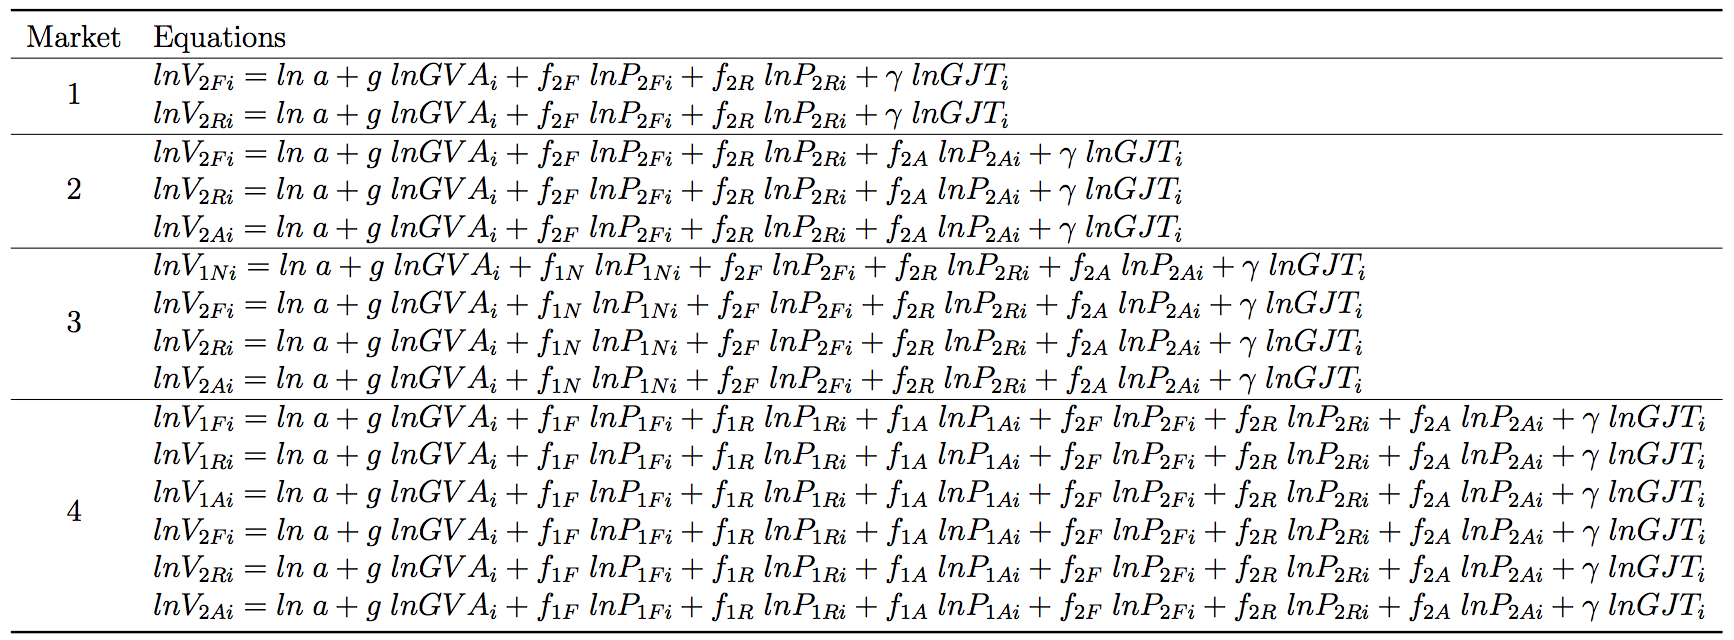
\includegraphics[scale=0.7]{eq-panel}
\caption*{Source: Own work}
\end{table} 
\end{landscape}


\renewcommand\chaptername{Appendix}
\chapter{Bayes estimation with weakly informative priors}
\label{apd:bayes_weakpriors}

% latex table generated in R 3.3.2 by xtable 1.8-2 package
% Mon Jul 31 09:29:49 2017
\begin{table} [H]
\caption{Comparison of elasticities estimates - Martket 1}
\label{tbl:mkt1_weak}
\centering
\begin{tabular}{rrrrrrrrrrr}
  \toprule 
 & \multicolumn{2}{c}{\textit{Bayes}} & & \multicolumn{2}{c}{\textit{SURE/OLS}} \\ 
\cline{2-3} \cline{5-6}
\\[-1.8ex] & $ln \; V_{2F}$ & $ln \; V_{2R}$ & & $ln \; V_{2F}$ & $ln \; V_{2R}$ \\ 
\hline \\[-1.8ex] 

  $f_{2F}$ &-1.33  & 0.70 & &-1.28 & 0.81\\
  		   & (0.05)  & (0.05) & & (0.05) & (0.05)\\ [0.2cm]
  $f_{2R}$ & 0.17 & -0.88  & & 0.17 & -0.89 \\
  			& (0.05) &  (0.05) & & (0.05) & (0.05)\\ [0.2cm]
  $g$ & 0.77 & 0.04 & & 0.49 & \cellcolor{gray!25}-0.52 \\
  		& (0.06) & (0.05) & & (0.7) & (0.7)\\ [0.2cm]
  $\gamma$ & -0.88 & -0.88 & & -0.98 & -1.06\\
  			& (0.04) & (0.04) & & (0.04) & (0.05)\\ [0.2cm]
  Constant & 6.05 & 11.43 & & 9.14 & 17.6\\
  			& (0.58) & (0.57) & & (0.71) & (0.73)\\ [0.2cm]
\bottomrule
\end{tabular}
\caption*{Source: Own work}
\end{table}


% latex table generated in R 3.3.2 by xtable 1.8-2 package
% Mon Jul 31 09:29:49 2017
\begin{table} 
\caption{Comparison of elasticities estimates - Martket 2}
\label{tbl:mkt2_weak}
\centering
\begin{tabular}{rrrrrrrrrrr}
  \toprule 
 & \multicolumn{3}{c}{\textit{Bayes}} && \multicolumn{3}{c}{\textit{SURE/OLS}} \\ 
\cline{2-4} \cline{6-8} 
\\[-1.8ex] & $ln \; V_{2F}$ & $ln \; V_{2R}$ & $ln \; V_{2A}$ & & $ln \; V_{2F}$ & $ln \; V_{2R}$ & $ln \; V_{2A}$ \\ 
\hline \\[-1.8ex] 

  $f_{2F}$ & -1.24  & \cellcolor{gray!25}-0.02 & \cellcolor{gray!25}-0.11 & & -1.24 & 0.03$^{\dagger}$ & \cellcolor{gray!25}-0.18\\
  		     & (0.06)  & (0.06) & (0.09) & & (0.06) & (0.06) & 0.10)\\ [0.2cm]
  $f_{2R}$ & \cellcolor{gray!25}-0.04 & -0.66 & 1.02 & & \cellcolor{gray!25}-0.06 & -0.60 & 1.03\\
  			   & (0.08) &  (0.08) & (0.12) & & (0.08) & (0.08) & (0.13)\\ [0.2cm]
  $f_{2A}$ & 0.15 & \cellcolor{gray!25}-0.10 & -0.47 & &0.15 & \cellcolor{gray!25}-0.10 & -0.47 \\
           & (0.04) & (0.04) & (0.06) & &(0.04) & (0.04) & (0.06)\\ [0.2cm]
  $g$      & 1.68 & 0.97 & 0.28  & &1.75 & 0.39 & 0.66\\
  		     & (0.07) & (0.07) & (0.09) & &(0.11) & (0.10) & (0.17)\\ [0.2cm]
  $\gamma$ & -1.25  & -1.05 & \cellcolor{gray!25}0.23 & &-1.23 & -1.21 & \cellcolor{gray!25}0.33\\
  			   & (0.06) & (0.06) & (0.09) & &(0.07) & (0.06) & (0.10)\\ [0.2cm]
  Constant &-0.37  & 5.39 & -1.34 & &-1.09$^{\dagger}$ & 11.72 & -5.53\\
  			   & (0.74) & (0.75) & (0.86) & &(1.15) & (1.09) & (1.77)\\ [0.2cm]
  % \hline
  % $\sigma$ & 1.36  & 1.29   & 2.10 &&&&\\
  % 		     & (0.01)& (0.01) & (0.02)&&&&\\
\bottomrule
Note: $^{\dagger}$ $p>0.1$
\end{tabular}
\caption*{Source: Own work}
\end{table}





% latex table generated in R 3.3.2 by xtable 1.8-2 package
% Mon Jul 31 09:29:49 2017
\begin{table}
\caption{Comparison of elasticities estimates - Martket 3}
\label{tbl:mkt3_weak_SCOTYORK}
\centering
\begin{tabular}{lrrrrrrrrrr}
  \toprule 
 & \multicolumn{4}{c}{\textit{Bayes}} && \multicolumn{4}{c}{\textit{SURE/OLS}} \\ 
\cline{2-5} \cline{7-10} 
\\[-1.8ex] & $ln \; V_{1N}$ & $ln \; V_{2F}$ & $ln \; V_{2R}$ & $ln \; V_{2A}$ & & $ln \; V_{1N}$ & $ln \; V_{2F}$ & $ln \; V_{2R}$ & $ln \; V_{2A}$ \\ 
\hline \\[-1.8ex] 

$f_{1N}$ & -0.82  & \cellcolor{gray!25}-0.42  & \cellcolor{gray!25}-0.41  & \cellcolor{gray!25}-0.47   && -0.84 & \cellcolor{gray!25}-0.43 & \cellcolor{gray!25}-0.44 & \cellcolor{gray!25}-0.50 \\
         & (0.06) & (0.05) & (0.05) & (0.07)  && (0.06) & (0.05) & (0.05) & (0.07) \\ [0.2cm]
$f_{2F}$ & 1.03   & -1.13  & 0.20   & 1.13    && 1.03 & -1.12 & 0.23 & 1.07 \\
         & (0.08) & (0.07) & (0.07) & (0.10)  && (0.09) & (0.07) & (0.07) & (0.10) \\ [0.2cm]
$f_{2R}$ & 1.73   & \cellcolor{gray!25}-0.06  & \cellcolor{gray!25}0.23   & 2.23    && 1.80 & \cellcolor{gray!25}-0.04 & \cellcolor{gray!25}0.34 & 2.28 \\ 
         & (0.10) & (0.09) & (0.08) & (0.13)  && (0.11) & (0.09) & (0.09) & (0.13) \\ [0.2cm]
$f_{2A}$ & 0.44   & 0.33   & 0.19   & -0.42   && 0.43 & 0.33 & 0.15 & -0.39 \\
         & (0.06) & (0.05) & (0.05) & (0.07)  && (0.06) & (0.05) & (0.05) & (0.07) \\ [0.2cm]
$g$      & 1.52   & 1.78   & 1.29   & 1.11    && 1.50 & 1.66 & 0.80 & 1.54 \\ 
         & (0.08) & (0.07) & (0.07) & (0.08)  && (0.11) & (0.09) & (0.09) & (0.13) \\ [0.2cm]
$\gamma$ & -3.25  & -1.57  & -2.17  & -2.06   && -3.30 & -1.60 & -2.31 & -2.01 \\ 
         & (0.08) & (0.06) & (0.06) & (0.09)  && (0.082) & (0.07) & (0.07) & (0.10) \\ [0.2cm]
Constant & 0.23   & 1.51   & 6.15   &  -2.21  && 0.62$^{\dagger}$ & 2.85 & 11.66 & -6.72 \\ 
         & (0.78) & (0.73) & (0.70) & (0.82)  && (1.23) & (1.00) & (0.95) & (1.45) \\ [0.2cm]
\bottomrule
\multicolumn{3}{l}{Note: $^{\dagger}$ $p>0.1$}
\end{tabular}
\caption*{Source: Own work}
\end{table}



% \begin{landscape}
% % latex table generated in R 3.3.2 by xtable 1.8-2 package
% Mon Jul 31 09:29:49 2017
\begin{table} [H]
\caption{Comparison of elasticities estimates - Martket 4}
\label{tbl:mkt4_weak_SCOTYORK}
\centering
\begin{tabular}{lrrrrrrrrrrrrr}
  \toprule 
 & \multicolumn{6}{c}{\textit{Bayes}} && \multicolumn{6}{c}{\textit{SURE/OLS}} \\ 
\cline{2-7} \cline{9-14} 
\\[-1.8ex] & $ln \; V_{1F}$ & $ln \; V_{1R}$ & $ln \; V_{1A}$ & $ln \; V_{2F}$ & $ln \; V_{2R}$ & $ln \; V_{2A}$ & & $ln \; V_{1F}$ & $ln \; V_{1R}$ & $ln \; V_{1A}$ & $ln \; V_{2F}$ & $ln \; V_{2R}$ & $ln \; V_{2A}$ \\ 
\hline \\[-1.8ex] 

$f_{1F}$ & -1.02  & 0.05   & 1.10   & 0.02   & 0.16   & 0.46   && -0.94   & \cellcolor{gray!25}-0.09$^{\dagger}$   & 1.20    & \cellcolor{gray!25}-0.50   & 0.01$^{\dagger}$    & 0.54 \\ 
         & (0.19) & (0.05) & (0.19) & (0.02) & (0.12) & (0.20) && (0.22)  & (0.27)  & (0.27)  & (0.20)  & (0.19)  & (0.26) \\ [0.08cm]
$f_{1R}$ & 0.05   & -0.51  & 0.02   & 0.01   & 0.21   & 0.03   && 0.06$^{\dagger}$    & -0.43   & \cellcolor{gray!25}-0.25   & \cellcolor{gray!25}-0.14   & 0.22    & \cellcolor{gray!25}-0.11 \\ 
         & (0.04) & (0.08) & (0.02) & (0.01) & (0.05) & (0.03) && (0.06)  & (0.08)  & (0.08)  & (0.06)  & (0.05)  & (0.07) \\ [0.08cm]
$f_{1A}$ & 0.24   & 0.02   & -0.09  & 0.04   & 0.39   & 0.80   && 0.28    & \cellcolor{gray!25}-0.99   & \cellcolor{gray!25}0.09$^{\dagger}$    & \cellcolor{gray!25}0.33    & 0.44    & 0.88 \\ 
         & (0.11) & (0.02) & (0.07) & (0.03) & (0.09) & (0.13) && (0.125) & (0.151) & (0.154) & (0.114) & (0.108) & (0.147) \\ [0.08cm]
$f_{2F}$ & 0.91   & 0.59   & 0.72   & -1.04  & 0.45   & 0.83   && 0.85    & 0.71    & 0.74    & \cellcolor{gray!25}-0.59   & 0.51    & 0.82 \\ 
         & (0.13) & (0.16) & (0.16) & (0.09) & (0.12) & (0.16) && (0.15)  & (0.18)  & (0.18)  & (0.14)  & (0.13)  & (0.17) \\ [0.08cm]
$f_{2R}$ & 0.87   & -0.13  & 0.43   & 0.05   & -1.32  & 0.64   && 0.67    & 0.00$^{\dagger}$    & 0.10$^{\dagger}$    & \cellcolor{gray!25}-0.32$^{\dagger}$   & -1.32   & 0.46$^{\dagger}$ \\ 
         & (0.22) & (0.23) & (0.23) & (0.04) & (0.19) & (0.26) && (0.27)  & (0.33)  & (0.34)  & (0.25)  & (0.23)  & (0.32) \\ [0.07cm]
$f_{2A}$ & 0.16   & 1.28   & 0.82   & 0.04   & 0.31   & -1.08  && 0.18$^{\dagger}$    & 2.37    & 1.04    & 0.03$^{\dagger}$    & 0.35    & -0.99 \\ 
         & (0.12) & (0.17) & (0.19) & (0.03) & (0.14) & (0.20) && (0.18)  & (0.22)  & (0.22)  & (0.16)  & (0.16)  & (0.21) \\ [0.07cm]
$g$      & 1.91   & 0.74   & 0.69   & 2.37   & 1.87   & 1.30   && 2.74    & 1.17    & 1.12    & 2.86    & 1.91    & 1.86 \\ 
         & (0.09) & (0.10) & (0.10) & (0.08) & (0.08) & (0.09) && (0.18)  & (0.22)  & (0.22)  & (0.17)  & (0.16)  & (0.22) \\ [0.07cm]
$\gamma$ & -2.66  & -1.42  & -2.18  & -2.14  & -2.07  & -2.05  && -2.39   & -1.79   & -2.03   & -1.71   & -2.07   & -1.90 \\ 
         & (0.13) & (0.15) & (0.16) & (0.10) & (0.12) & (0.16) && (0.15)  & (0.18)  & (0.18)  & (0.14)  & (0.13)  & (0.18) \\[0.07cm]
Constant & -2.40  & -0.64  & -0.84  & -2.27  & -0.01  & -1.17  && -11.98  & -3.34$^{\dagger}$   & -5.89   & -8.38   & -0.38$^{\dagger}$   & -7.47 \\ 
         & (0.89) & (0.93) & (0.94) & (0.79) & 0.81   & (0.04) && (2.09)  & (2.53)  & (2.57)  & (1.91)  & (1.80)  & (2.46) \\ 
\bottomrule
\multicolumn{3}{l}{Note: $^{\dagger}$ $p>0.1$}
\end{tabular}
\caption*{Source: Own work}
\end{table}

% \end{landscape}

\begin{sidewaystable}
% latex table generated in R 3.3.2 by xtable 1.8-2 package
% Mon Jul 31 09:29:49 2017
\begin{table} [H]
\caption{Comparison of elasticities estimates - Martket 4}
\label{tbl:mkt4_weak_SCOTYORK}
\centering
\begin{tabular}{lrrrrrrrrrrrrr}
  \toprule 
 & \multicolumn{6}{c}{\textit{Bayes}} && \multicolumn{6}{c}{\textit{SURE/OLS}} \\ 
\cline{2-7} \cline{9-14} 
\\[-1.8ex] & $ln \; V_{1F}$ & $ln \; V_{1R}$ & $ln \; V_{1A}$ & $ln \; V_{2F}$ & $ln \; V_{2R}$ & $ln \; V_{2A}$ & & $ln \; V_{1F}$ & $ln \; V_{1R}$ & $ln \; V_{1A}$ & $ln \; V_{2F}$ & $ln \; V_{2R}$ & $ln \; V_{2A}$ \\ 
\hline \\[-1.8ex] 

$f_{1F}$ & -1.02  & 0.05   & 1.10   & 0.02   & 0.16   & 0.46   && -0.94   & \cellcolor{gray!25}-0.09$^{\dagger}$   & 1.20    & \cellcolor{gray!25}-0.50   & 0.01$^{\dagger}$    & 0.54 \\ 
         & (0.19) & (0.05) & (0.19) & (0.02) & (0.12) & (0.20) && (0.22)  & (0.27)  & (0.27)  & (0.20)  & (0.19)  & (0.26) \\ [0.08cm]
$f_{1R}$ & 0.05   & -0.51  & 0.02   & 0.01   & 0.21   & 0.03   && 0.06$^{\dagger}$    & -0.43   & \cellcolor{gray!25}-0.25   & \cellcolor{gray!25}-0.14   & 0.22    & \cellcolor{gray!25}-0.11 \\ 
         & (0.04) & (0.08) & (0.02) & (0.01) & (0.05) & (0.03) && (0.06)  & (0.08)  & (0.08)  & (0.06)  & (0.05)  & (0.07) \\ [0.08cm]
$f_{1A}$ & 0.24   & 0.02   & -0.09  & 0.04   & 0.39   & 0.80   && 0.28    & \cellcolor{gray!25}-0.99   & \cellcolor{gray!25}0.09$^{\dagger}$    & \cellcolor{gray!25}0.33    & 0.44    & 0.88 \\ 
         & (0.11) & (0.02) & (0.07) & (0.03) & (0.09) & (0.13) && (0.125) & (0.151) & (0.154) & (0.114) & (0.108) & (0.147) \\ [0.08cm]
$f_{2F}$ & 0.91   & 0.59   & 0.72   & -1.04  & 0.45   & 0.83   && 0.85    & 0.71    & 0.74    & \cellcolor{gray!25}-0.59   & 0.51    & 0.82 \\ 
         & (0.13) & (0.16) & (0.16) & (0.09) & (0.12) & (0.16) && (0.15)  & (0.18)  & (0.18)  & (0.14)  & (0.13)  & (0.17) \\ [0.08cm]
$f_{2R}$ & 0.87   & -0.13  & 0.43   & 0.05   & -1.32  & 0.64   && 0.67    & 0.00$^{\dagger}$    & 0.10$^{\dagger}$    & \cellcolor{gray!25}-0.32$^{\dagger}$   & -1.32   & 0.46$^{\dagger}$ \\ 
         & (0.22) & (0.23) & (0.23) & (0.04) & (0.19) & (0.26) && (0.27)  & (0.33)  & (0.34)  & (0.25)  & (0.23)  & (0.32) \\ [0.07cm]
$f_{2A}$ & 0.16   & 1.28   & 0.82   & 0.04   & 0.31   & -1.08  && 0.18$^{\dagger}$    & 2.37    & 1.04    & 0.03$^{\dagger}$    & 0.35    & -0.99 \\ 
         & (0.12) & (0.17) & (0.19) & (0.03) & (0.14) & (0.20) && (0.18)  & (0.22)  & (0.22)  & (0.16)  & (0.16)  & (0.21) \\ [0.07cm]
$g$      & 1.91   & 0.74   & 0.69   & 2.37   & 1.87   & 1.30   && 2.74    & 1.17    & 1.12    & 2.86    & 1.91    & 1.86 \\ 
         & (0.09) & (0.10) & (0.10) & (0.08) & (0.08) & (0.09) && (0.18)  & (0.22)  & (0.22)  & (0.17)  & (0.16)  & (0.22) \\ [0.07cm]
$\gamma$ & -2.66  & -1.42  & -2.18  & -2.14  & -2.07  & -2.05  && -2.39   & -1.79   & -2.03   & -1.71   & -2.07   & -1.90 \\ 
         & (0.13) & (0.15) & (0.16) & (0.10) & (0.12) & (0.16) && (0.15)  & (0.18)  & (0.18)  & (0.14)  & (0.13)  & (0.18) \\[0.07cm]
Constant & -2.40  & -0.64  & -0.84  & -2.27  & -0.01  & -1.17  && -11.98  & -3.34$^{\dagger}$   & -5.89   & -8.38   & -0.38$^{\dagger}$   & -7.47 \\ 
         & (0.89) & (0.93) & (0.94) & (0.79) & 0.81   & (0.04) && (2.09)  & (2.53)  & (2.57)  & (1.91)  & (1.80)  & (2.46) \\ 
\bottomrule
\multicolumn{3}{l}{Note: $^{\dagger}$ $p>0.1$}
\end{tabular}
\caption*{Source: Own work}
\end{table}

\end{sidewaystable}
% \renewcommand\chaptername{Appendix}
\chapter{Bayesian constrained estimation - Quantiles}
\label{apd:bayes_quants}


% \section{Market 1}

% latex table generated in R 3.3.2 by xtable 1.8-2 package
% Sun Aug  6 17:25:21 2017
\begin{table}[H]
\caption{Marginal posterior distributions's quantiles - $ln V_{2F}$,  Market 1}
\centering
\begin{tabular}{rrrrrrrrrrr}
  \toprule
            & mean  & sd   & 2.5\% & 25\%  & 50\%  & 75\%  & 97.5\%\\
  \hline
  $f_{2F}$  & -1.32 & 0.05 & -1.42 & -1.36 & -1.32 & -1.29 & -1.23 \\
  $f_{2R}$  & 0.17  & 0.05 & 0.07  & 0.13  & 0.17  & 0.20  & 0.26  \\
  $g$       & 0.77  & 0.05 & 0.67  & 0.73  & 0.77  & 0.81  & 0.87  \\
  $\gamma$  & -0.89 & 0.04 & -0.97 & -0.92 & -0.89 & -0.86 & -0.80 \\
  Constant  & 6.10  & 0.57 & 5.02  & 5.72  & 6.10  & 6.50  & 7.19  \\
     \bottomrule
\end{tabular}
\caption*{Source: Own work}
\end{table}

\vspace{-2em}
% latex table generated in R 3.3.2 by xtable 1.8-2 package
% Sun Aug  6 17:49:28 2017
\begin{table}[H]
\caption{Marginal posterior distributions's quantiles - $ln V_{2R}$,  Market 1}
\centering
\begin{tabular}{rrrrrrrrrrr}
  \toprule
          & mean  & sd   & 2.5\% & 25\%  & 50\%  & 75\%  & 97.5\%\\
 \hline

$f_{2F}$  & 0.70  & 0.05 & 0.61  & 0.67  & 0.70  & 0.74  & 0.80  \\ 
$f_{2R}$  & -0.89 & 0.05 & -0.99 & -0.92 & -0.89 & -0.86 & -0.79 \\ 
$g$       & 0.06  & 0.04 & 0.00  & 0.02  & 0.05  & 0.09  & 0.15  \\ 
$\gamma$  & -0.88 & 0.05 & -0.97 & -0.91 & -0.88 & -0.85 & -0.80 \\ 
Constant  & 11.27 & 0.47 & 10.22 & 10.96 & 11.32 & 11.62 & 12.01 \\ 
     \bottomrule
\end{tabular}
\caption*{Source: Own work}
\end{table}

\vspace{-2em}

% \section{Market 2}

% latex table generated in R 3.3.2 by xtable 1.8-2 package
% Sun Aug  6 20:06:34 2017
\begin{table}[H]
\caption{Marginal posterior distributions's quantiles - $ln V_{2F}$,  Market 2}
\centering
\begin{tabular}{rrrrrrrrrrr}
  \toprule
            & mean   & sd   & 2.5\% & 25\%  & 50\%  & 75\%  & 97.5\% \\ 
  \hline

  $f_{2F}$  & -1.29  & 0.05 & -1.38 & -1.32 & -1.29 & -1.26 & -1.21 \\ 
  $f_{2R}$  & 0.05   & 0.04 & 0.00  & 0.02  & 0.04  & 0.08  & 0.16  \\ 
  $f_{2A}$  & 0.14   & 0.04 & 0.06  & 0.11  & 0.14  & 0.16  & 0.21  \\ 
  $g$       & 1.68   & 0.07 & 1.53  & 1.64  & 1.69  & 1.73  & 1.82  \\ 
  $\gamma$  & -1.28  & 0.06 & -1.39 & -1.32 & -1.28 & -1.24 & -1.17 \\ 
  Constant  & -0.28  & 0.76 & -1.78 & -0.77 & -0.29 & 0.22  & 1.27  \\ 
     \bottomrule
\end{tabular}
\caption*{Source: Own work}
\end{table}

\vspace{-2em}
% latex table generated in R 3.3.2 by xtable 1.8-2 package
% Sun Aug  6 20:06:34 2017
\begin{table}[H]
\caption{Marginal posterior distributions's quantiles - $ln V_{2R}$,  Market 2}
\centering
\begin{tabular}{rrrrrrrrrrr}
  \toprule
           & mean  & sd   & 2.5\% & 25\%  & 50\%  & 75\%  & 97.5\%\\ 
  \hline
  $f_{2F}$ & 0.04  & 0.03 & 0.00  & 0.01  & 0.03  & 0.05  & 0.11  \\ 
  $f_{2R}$ & -0.80 & 0.05 & -0.91 & -0.84 & -0.80 & -0.77 & -0.71 \\ 
  $f_{2A}$ & 0.01  & 0.01 & 0.00  & 0.00  & 0.01  & 0.01  & 0.04  \\ 
  $g$      & 0.96  & 0.07 & 0.83  & 0.92  & 0.96  & 1.01  & 1.10  \\ 
  $\gamma$ & -1.07 & 0.06 & -1.18 & -1.11 & -1.07 & -1.03 & -0.95 \\ 
  Constant & 5.46  & 0.71 & 4.06  & 4.99  & 5.46  & 5.95  & 6.82  \\ 
     \bottomrule
\end{tabular}
\caption*{Source: Own work}
\end{table}

\vspace{-2em}
% latex table generated in R 3.3.2 by xtable 1.8-2 package
% Sun Aug  6 20:06:35 2017
\begin{table}[H]
\caption{Marginal posterior distributions's quantiles - $ln V_{2A}$,  Market 2}
\centering
\begin{tabular}{rrrrrrrrrrr}
  \toprule
           & mean  & sd   & 2.5\% & 25\%  & 50\%  & 75\%  & 97.5\% \\ 
  \hline
  $f_{2F}$ & 0.05  & 0.04 & 0.00  & 0.02  & 0.04  & 0.07  & 0.15  \\ 
  $f_{2R}$ & 1.01  & 0.08 & 0.85  & 0.96  & 1.01  & 1.07  & 1.16  \\ 
  $f_{2A}$ & -0.46 & 0.06 & -0.57 & -0.50 & -0.46 & -0.42 & -0.34 \\ 
  $g$      & 0.29  & 0.08 & 0.13  & 0.24  & 0.29  & 0.35  & 0.45  \\ 
  $\gamma$ & -0.03 & 0.03 & -0.10 & -0.04 & -0.02 & -0.01 & -0.00 \\ 
  Constant & -0.61 & 0.82 & -2.22 & -1.18 & -0.63 & -0.07 & 0.99  \\ 
     \bottomrule
\end{tabular}
\caption*{Source: Own work}
\end{table}


% \section{Market 3}

% latex table generated in R 3.3.2 by xtable 1.8-2 package
% Thu Aug 10 13:29:28 2017
\begin{table}[H]
\caption{Marginal posterior distributions's quantiles - $ln V_{1N}$,  Market 3}
\centering
\begin{tabular}{rrrrrrrrrrr}
  \toprule
          & mean   & sd   & 2.5\% & 25\%  & 50\%  & 75\%  & 97.5\% \\ 
  \hline
  $f_{1N}$ & -0.82  & 0.06 & -0.94 & -0.86 & -0.82 & -0.78 & -0.70 \\ 
  $f_{2F}$ & 1.04   & 0.09 & 0.87  & 0.98  & 1.04  & 1.09  & 1.21  \\ 
  $f_{2R}$ & 1.73   & 0.11 & 1.51  & 1.65  & 1.73  & 1.81  & 1.94  \\ 
  $f_{2A}$ & 0.44   & 0.06 & 0.32  & 0.39  & 0.44  & 0.48  & 0.56  \\ 
  $g$      & 1.53   & 0.07 & 1.38  & 1.48  & 1.53  & 1.58  & 1.67  \\ 
  $\gamma$ & -3.25  & 0.08 & -3.40 & -3.30 & -3.25 & -3.20 & -3.10 \\ 
  Constant & 0.20   & 0.76 & -1.30 & -0.30 & 0.20  & 0.69  & 1.71  \\ 
     \bottomrule
\end{tabular}
\caption*{Source: Own work}
\end{table}

\vspace{-2em}
% latex table generated in R 3.3.2 by xtable 1.8-2 package
% Thu Aug 10 13:29:28 2017
\begin{table}[H]
\caption{Marginal posterior distributions's quantiles - $ln V_{2F}$,  Market 3}
\centering
\begin{tabular}{rrrrrrrrrrr}
  \toprule
           & mean  & sd   & 2.5\% & 25\%  & 50\%  & 75\%  & 97.5\%\\ 
  \hline
  $f_{1N}$ & 0.00  & 0.00 & 0.00  & 0.00  & 0.00  & 0.01  & 0.02  \\ 
  $f_{2F}$ & -1.40 & 0.05 & -1.50 & -1.43 & -1.40 & -1.37 & -1.29 \\ 
  $f_{2R}$ & 0.02  & 0.02 & 0.00  & 0.01  & 0.02  & 0.03  & 0.07  \\ 
  $f_{2A}$ & 0.18  & 0.05 & 0.08  & 0.15  & 0.18  & 0.22  & 0.28  \\ 
  $g$      & 1.72  & 0.07 & 1.60  & 1.67  & 1.72  & 1.77  & 1.86  \\ 
  $\gamma$ & -1.55 & 0.06 & -1.66 & -1.59 & -1.55 & -1.51 & -1.44 \\ 
  Constant & 1.56  & 0.72 & 0.17  & 1.05  & 1.57  & 2.10  & 2.87  \\ 
     \bottomrule
\end{tabular}
\caption*{Source: Own work}
\end{table}

\vspace{-2em}
% latex table generated in R 3.3.2 by xtable 1.8-2 package
% Thu Aug 10 14:00:32 2017
\begin{table}[H]
\caption{Marginal posterior distributions's quantiles - $ln V_{2R}$,  Market 3}
\centering
\begin{tabular}{rrrrrrrrrrr}
  \toprule
          & mean  & sd   & 2.5\% & 25\%  & 50\%  & 75\%  & 97.5\%\\ 
  \hline
  $f_{1N}$ & 0.01  & 0.01 & 0.00  & 0.00  & 0.00  & 0.01  & 0.02  \\ 
  $f_{2F}$ & 0.16  & 0.05 & 0.06  & 0.12  & 0.16  & 0.19  & 0.27  \\ 
  $f_{2R}$ & -0.06 & 0.05 & -0.17 & -0.09 & -0.05 & -0.02 & -0.00 \\ 
  $f_{2A}$ & 0.10  & 0.04 & 0.02  & 0.06  & 0.10  & 0.13  & 0.19  \\ 
  $g$      & 1.24  & 0.07 & 1.12  & 1.20  & 1.24  & 1.29  & 1.37  \\ 
  $\gamma$ & -2.05 & 0.06 & -2.16 & -2.09 & -2.05 & -2.01 & -1.93 \\ 
  Constant & 5.80  & 0.68 & 4.45  & 5.35  & 5.81  & 6.26  & 7.11  \\ 
     \bottomrule
\end{tabular}
\caption*{Source: Own work}
\end{table}

\vspace{-2em}
% latex table generated in R 3.3.2 by xtable 1.8-2 package
% Thu Aug 10 13:29:29 2017
\begin{table}[H]
\caption{Marginal posterior distributions's quantiles - $ln V_{2A}$,  Market 3}
\centering
\begin{tabular}{rrrrrrrrrrr}
  \toprule
          & mean  & sd   & 2.5\% & 25\%  & 50\%  & 75\%  & 97.5\%\\ 
  \hline
  $f_{1N}$ & 0.01  & 0.01 & 0.00  & 0.00  & 0.01  & 0.01  & 0.04  \\ 
  $f_{2F}$ & 1.04  & 0.10 & 0.84  & 0.97  & 1.04  & 1.10  & 1.23  \\ 
  $f_{2R}$ & 1.97  & 0.11 & 1.74  & 1.89  & 1.97  & 2.04  & 2.19  \\ 
  $f_{2A}$ & -0.54 & 0.07 & -0.68 & -0.59 & -0.54 & -0.49 & -0.40 \\ 
  $g$      & 1.03  & 0.08 & 0.88  & 0.98  & 1.03  & 1.09  & 1.20  \\ 
  $\gamma$ & -1.94 & 0.09 & -2.13 & -2.01 & -1.94 & -1.88 & -1.76 \\ 
  Constant & -2.37 & 0.85 & -4.07 & -2.93 & -2.39 & -1.84 & -0.64 \\ 
     \bottomrule
\end{tabular}
\caption*{Source: Own work}
\end{table}


% \section{Market 4}
% latex table generated in R 3.3.2 by xtable 1.8-2 package
% Thu Aug 10 16:24:07 2017
\begin{table}[H]
\caption{Marginal posterior distributions's quantiles - $ln V_{1F}$,  Market 4}
\centering
\begin{tabular}{rrrrrrrrrrr}
  \toprule
          & mean  & sd   & 2.5\% & 25\%  & 50\%  & 75\%  & 97.5\%\\ 
  \hline
  $f_{1F}$ & -1.02 & 0.19 & -1.39 & -1.15 & -1.02 & -0.89 & -0.67 \\ 
  $f_{1R}$ & 0.05  & 0.04 & 0.00  & 0.02  & 0.04  & 0.08  & 0.15  \\ 
  $f_{1A}$ & 0.24  & 0.11 & 0.04  & 0.16  & 0.23  & 0.31  & 0.45  \\ 
  $f_{2F}$ & 0.91  & 0.13 & 0.65  & 0.82  & 0.91  & 1.00  & 1.17  \\ 
  $f_{2R}$ & 0.87  & 0.22 & 0.43  & 0.73  & 0.88  & 1.01  & 1.30  \\ 
  $f_{2A}$ & 0.16  & 0.12 & 0.01  & 0.07  & 0.14  & 0.23  & 0.44  \\ 
  $g$      & 1.91  & 0.09 & 1.75  & 1.85  & 1.91  & 1.97  & 2.08  \\ 
  $\gamma$ & -2.66 & 0.13 & -2.92 & -2.75 & -2.66 & -2.58 & -2.41 \\ 
  Constant & -2.40 & 0.89 & -4.18 & -2.99 & -2.40 & -1.81 & -0.65 \\ 
     \bottomrule
\end{tabular}
\caption*{Source: Own work}
\end{table}

\vspace{-2.5em}
% latex table generated in R 3.3.2 by xtable 1.8-2 package
% Thu Aug 10 16:38:19 2017
\begin{table}[H]
\caption{Marginal posterior distributions's quantiles - $ln V_{1R}$,  Market 4}
\centering
\begin{tabular}{rrrrrrrrrrr}
  \toprule
           & mean  & sd   & 2.5\% & 25\%  & 50\%  & 75\%  & 97.5\% \\ 
  \hline
  $f_{1F}$ & 0.05  & 0.05 & 0.00  & 0.01  & 0.03  & 0.07  & 0.18  \\ 
  $f_{1R}$ & -0.51 & 0.08 & -0.65 & -0.56 & -0.51 & -0.46 & -0.35 \\ 
  $f_{1A}$ & 0.02  & 0.02 & 0.00  & 0.00  & 0.01  & 0.03  & 0.06  \\ 
  $f_{2F}$ & 0.59  & 0.16 & 0.26  & 0.48  & 0.59  & 0.70  & 0.91  \\ 
  $f_{2R}$ & -0.13 & 0.23 & -0.59 & -0.29 & -0.14 & 0.02  & 0.33  \\ 
  $f_{2A}$ & 1.28  & 0.17 & 0.94  & 1.17  & 1.28  & 1.40  & 1.63  \\ 
  $g$      & 0.74  & 0.10 & 0.55  & 0.68  & 0.75  & 0.81  & 0.92  \\ 
  $\gamma$ & -1.42 & 0.15 & -1.71 & -1.52 & -1.42 & -1.31 & -1.11 \\ 
  Constant & -0.64 & 0.93 & -2.43 & -1.27 & -0.67 & -0.02 & 1.19  \\ 
     \bottomrule
\end{tabular}
\caption*{Source: Own work}
\end{table}

\vspace{-2.5em}
% latex table generated in R 3.3.2 by xtable 1.8-2 package
% Fri Aug 11 10:24:46 2017
\begin{table}[H]
\caption{Marginal posterior distributions's quantiles - $ln V_{1A}$,  Market 4}
\centering
\begin{tabular}{rrrrrrrrrrr}
  \toprule
           & mean  & sd & 2.5\%   & 25\%  & 50\%  & 75\%  & 97.5\%\\ 
  \hline
  $f_{1F}$ & 1.10  & 0.19 & 0.70  & 0.97  & 1.09  & 1.23  & 1.47  \\ 
  $f_{1R}$ & 0.02  & 0.02 & 0.00  & 0.01  & 0.02  & 0.03  & 0.07  \\ 
  $f_{1A}$ & -0.09 & 0.07 & -0.27 & -0.13 & -0.08 & -0.04 & -0.00 \\ 
  $f_{2F}$ & 0.72  & 0.16 & 0.42  & 0.62  & 0.73  & 0.83  & 1.02  \\ 
  $f_{2R}$ & 0.43  & 0.23 & 0.04  & 0.25  & 0.41  & 0.59  & 0.91  \\ 
  $f_{2A}$ & 0.82  & 0.19 & 0.45  & 0.70  & 0.82  & 0.95  & 1.20  \\ 
  $g$      & 0.69  & 0.10 & 0.49  & 0.62  & 0.69  & 0.76  & 0.89  \\ 
  $\gamma$ & -2.18 & 0.16 & -2.47 & -2.29 & -2.18 & -2.08 & -1.86 \\ 
  Constant & -0.84 & 0.94 & -2.73 & -1.48 & -0.83 & -0.22 & 1.08  \\ 
     \bottomrule
\end{tabular}
\caption*{Source: Own work}
\end{table}

\vspace{-2.5em}
% latex table generated in R 3.3.2 by xtable 1.8-2 package
% Fri Aug 11 11:47:28 2017
\begin{table}[H]
\caption{Marginal posterior distributions's quantiles - $ln V_{2F}$,  Market 4}
\centering
\begin{tabular}{rrrrrrrrrrr}
  \toprule
           & mean  & sd   & 2.5\% & 25\%  & 50\%  & 75\%  & 97.5\%\\ 
  \hline

  $f_{1F}$ & 0.02  & 0.02 & 0.00  & 0.01  & 0.02  & 0.03  & 0.09  \\ 
  $f_{1R}$ & 0.01  & 0.01 & 0.00  & 0.00  & 0.01  & 0.02  & 0.04  \\ 
  $f_{1A}$ & 0.04  & 0.03 & 0.00  & 0.01  & 0.03  & 0.05  & 0.10  \\ 
  $f_{2F}$ & -1.04 & 0.09 & -1.22 & -1.09 & -1.04 & -0.98 & -0.87 \\ 
  $f_{2R}$ & 0.05  & 0.04 & 0.00  & 0.01  & 0.03  & 0.06  & 0.17  \\ 
  $f_{2A}$ & 0.04  & 0.03 & 0.00  & 0.01  & 0.03  & 0.05  & 0.13  \\ 
  $g$      & 2.37  & 0.08 & 2.21  & 2.31  & 2.37  & 2.42  & 2.52  \\ 
  $\gamma$ & -2.14 & 0.10 & -2.33 & -2.21 & -2.13 & -2.06 & -1.94 \\ 
  Constant & -2.27 & 0.79 & -3.93 & -2.80 & -2.24 & -1.72 & -0.82 \\ 
     \bottomrule
\end{tabular}
\caption*{Source: Own work}
\end{table}

\vspace{-2.5em}
% latex table generated in R 3.3.2 by xtable 1.8-2 package
% Fri Aug 11 10:57:41 2017
\begin{table}[H]
\caption{Marginal posterior distributions's quantiles - $ln V_{2R}$,  Market 4}
\centering
\begin{tabular}{rrrrrrrrrrr}
  \toprule
         & mean   & sd   & 2.5\% & 25\%  & 50\%  & 75\%  & 97.5\%\\ 
  \hline
  $f_{1F}$ & 0.16  & 0.12 & 0.01  & 0.07  & 0.14  & 0.23  & 0.43 \\ 
  $f_{1R}$ & 0.21  & 0.05 & 0.11  & 0.18  & 0.21  & 0.25  & 0.32 \\ 
  $f_{1A}$ & 0.39  & 0.09 & 0.21  & 0.33  & 0.40  & 0.45  & 0.56 \\ 
  $f_{2F}$ & 0.45  & 0.12 & 0.22  & 0.37  & 0.45  & 0.53  & 0.66 \\ 
  $f_{2R}$ & -1.32 & 0.19 & -1.71 & -1.45 & -1.32 & -1.19 & -0.97\\ 
  $f_{2A}$ & 0.31  & 0.14 & 0.05  & 0.20  & 0.30  & 0.40  & 0.60 \\ 
  $g$      & 1.87  & 0.08 & 1.73  & 1.82  & 1.87  & 1.93  & 2.03 \\ 
  $\gamma$ & -2.07 & 0.12 & -2.31 & -2.15 & -2.07 & -1.99 & -1.84\\ 
  Constant & -0.01 & 0.81 & -1.59 & -0.55 & 0.03  & 0.56  & 1.53 \\ 
     \bottomrule
\end{tabular}
\caption*{Source: Own work}
\end{table}

\vspace{-2.5em}
% latex table generated in R 3.3.2 by xtable 1.8-2 package
% Fri Aug 11 09:55:58 2017
\begin{table}[H]
\caption{Marginal posterior distributions's quantiles - $ln V_{2A}$,  Market 4}
\centering
\begin{tabular}{rrrrrrrrrrr}
  \toprule
           & mean  & sd   & 2.5\% & 25\%  & 50\%  & 75\%  & 97.5\% \\ 
  \hline
  $f_{1F}$ & 0.46  & 0.20 & 0.07  & 0.32  & 0.46  & 0.59  & 0.84  \\ 
  $f_{1R}$ & 0.03  & 0.03 & 0.00  & 0.01  & 0.02  & 0.04  & 0.10  \\ 
  $f_{1A}$ & 0.80  & 0.13 & 0.54  & 0.72  & 0.81  & 0.89  & 1.07  \\ 
  $f_{2F}$ & 0.83  & 0.16 & 0.53  & 0.72  & 0.83  & 0.94  & 1.15  \\ 
  $f_{2R}$ & 0.64  & 0.26 & 0.14  & 0.46  & 0.63  & 0.82  & 1.16  \\ 
  $f_{2A}$ & -1.08 & 0.20 & -1.47 & -1.22 & -1.08 & -0.95 & -0.71 \\ 
  $g$      & 1.30  & 0.09 & 1.13  & 1.24  & 1.30  & 1.36  & 1.50  \\ 
  $\gamma$ & -2.05 & 0.16 & -2.37 & -2.16 & -2.05 & -1.94 & -1.75 \\ 
  Constant & -1.17 & 0.90 & -3.03 & -1.73 & -1.15 & -0.59 & 0.60  \\ 
     \bottomrule
\end{tabular}
\caption*{Source: Own work}
\end{table}

% 
\renewcommand\chaptername{Appendix}
\chapter{Bayes estimation with constrained priors - Autocorrelation and convergence measures}
\label{apd:bayes_autocorr_convergence}

% latex table generated in R 3.3.2 by xtable 1.8-2 package
% Sat Aug  5 10:10:51 2017
\begin{table}[ht]
\caption{Autocorrelation and convergence measures - Market 1}
\label{mkt1_T_autocorr_convergence}
\centering
\begin{tabular}{lrrrrr}
\toprule 
 & \multicolumn{5}{c}{\textit{Dependent variable:}} \\ 
\cline{2-6} 
\\[-1.8ex] & \multicolumn{2}{c}{$ln \; V_{2F}$} & & \multicolumn{2}{c}{ $ln \; V_{2R}$}\\ 
\cline{2-3} \cline{5-6}
 & $\hat{R}$ & $n_{\text{eff}}$ & &$\hat{R}$ & $n_{\text{eff}}$ \\ 
  \midrule

  $f_{2F}$ & 1.0 & 1650 & & 1.0 & 402 \\ 
  $f_{2R}$ & 1.0 & 1692 & & 1.0 & 821 \\ 
  $g$      & 1.0 & 1561 & & 1.0 & 719 \\ 
  $\gamma$ & 1.0 & 1778 & & 1.0 & 432 \\ 
  Constant & 1.0 & 1477 & & 1.0 & 702 \\ 
   \hline
   Iter    & \multicolumn{2}{c}{2,000} && \multicolumn{2}{c}{2,000} \\
   Thin    & \multicolumn{2}{c}{1} && \multicolumn{2}{c}{1} \\
   \bottomrule
\end{tabular}
\caption*{Source: Own work}
\end{table}
\vspace{-2em}
% latex table generated in R 3.3.2 by xtable 1.8-2 package
% Sat Aug  5 10:10:51 2017
\begin{table}[H]
\caption{Autocorrelation and Convergence Measures - Market 2}
\label{mkt2_T_autocorr_convergence}
\centering
\begin{tabular}{lrrrrrrrr}
\toprule 
 & \multicolumn{8}{c}{\textit{Dependent variable:}} \\ 
\cline{2-9} 
\\[-1.8ex] & \multicolumn{2}{c}{$ln \; V_{2F}$} & & \multicolumn{2}{c}{ $ln \; V_{2R}$} & &  \multicolumn{2}{c}{ $ln \; V_{2A}$}\\ 
\cline{2-3} \cline{5-6} \cline{8-9}
 & $\hat{R}$ & $n_{\text{eff}}$ & & $\hat{R}$ & $n_{\text{eff}}$  & & $\hat{R}$ & $n_{\text{eff}}$ \\ 
\hline \\[-1.8ex] 
  $f_{2F}$ & 1.0 & 405 & & 1.0 & 464 & & 1.0 & 529 \\ 
  $f_{2R}$ & 1.0 & 251 & & 1.0 & 414 & & 1.0 & 493 \\ 
  $f_{2A}$ & 1.0 & 614 & & 1.0 & 702 & & 1.0 & 634 \\ 
  $g$      & 1.0 & 315 & & 1.0 & 561 & & 1.0 & 555 \\ 
  $\gamma$ & 1.0 & 400 & & 1.0 & 525 & & 1.0 & 912 \\ 
  Constant & 1.0 & 310 & & 1.0 & 548 & & 1.0 & 500 \\
   \hline
   Iter    & \multicolumn{2}{c}{2,000} && \multicolumn{2}{c}{10,000} && \multicolumn{2}{c}{10,000} \\
   Thin    & \multicolumn{2}{c}{1} && \multicolumn{2}{c}{1} && \multicolumn{2}{c}{1} \\
   \bottomrule
\end{tabular}
\caption*{Source: Own work}
\end{table}
% latex table generated in R 3.3.2 by xtable 1.8-2 package
% Sat Aug  5 10:10:51 2017
\begin{table}[ht]
\caption{Autocorrelation and Convergence Measures - Market 3}
\label{mkt3_T_autocorr_convergence_SCOTYORK}
\centering
\begin{tabular}{lrrrrrrrrrrr}
\toprule 
 & \multicolumn{11}{c}{\textit{Dependent variable:}} \\ 
\cline{2-12} 
\\[-1.8ex] & \multicolumn{2}{c}{$ln \; V_{1N}$} & &\multicolumn{2}{c}{$ln \; V_{2F}$} & & \multicolumn{2}{c}{ $ln \; V_{2R}$} & &  \multicolumn{2}{c}{ $ln \; V_{2A}$}\\ 
\cline{2-3} \cline{5-6} \cline{8-9} \cline{11-12}
 & $\hat{R}$ & $n_{\text{eff}}$ & & $\hat{R}$ & $n_{\text{eff}}$  & & $\hat{R}$ & $n_{\text{eff}}$ & & $\hat{R}$ & $n_{\text{eff}}$ \\  
\hline \\[-1.8ex] 
  $f_{1N}$ & 1.0 & 2712 & & 1.0 & 492 & & 1.0 & 826 & & 1.0 & 939 \\
  $f_{2F}$ & 1.0 & 2350 & & 1.0 & 278 & & 1.0 & 637 & & 1.0 & 1031\\
  $f_{2R}$ & 1.0 & 2203 & & 1.0 & 205 & & 1.0 & 561 & & 1.0 & 948 \\
  $f_{2A}$ & 1.0 & 3000 & & 1.0 & 294 & & 1.0 & 678 & & 1.0 & 1187\\
  $g$      & 1.0 & 2128 & & 1.0 & 147 & & 1.0 & 376 & & 1.0 & 668 \\
  $\gamma$ & 1.0 & 2708 & & 1.0 & 367 & & 1.0 & 559 & & 1.0 & 945 \\
  Constant & 1.0 & 2130 & & 1.0 & 140 & & 1.0 & 409 & & 1.0 & 756 \\
   \hline
   Iter   & \multicolumn{2}{c}{2,000} && \multicolumn{2}{c}{10,000} && \multicolumn{2}{c}{10,000} && \multicolumn{2}{c}{10,000} \\
   Thin   & \multicolumn{2}{c}{1} && \multicolumn{2}{c}{5} && \multicolumn{2}{c}{1} && \multicolumn{2}{c}{5} \\
   \bottomrule
\end{tabular}
\caption*{Source: Own work}
\end{table}
% latex table generated in R 3.3.2 by xtable 1.8-2 package
% Sat Aug  5 10:10:51 2017
\begin{table}[H]
\caption{Autocorrelation and Convergence Measures - Market 4}
\label{mkt4_T_autocorr_convergence_SCOTYORK}
\centering
\begin{tabular}{lrrrrrrrrrrrrrrrrrrrr}
\toprule 
 & \multicolumn{17}{c}{\textit{Dependent variable:}} \\ 
\cline{2-21} 
\\[-1.8ex] & \multicolumn{2}{c}{$ln \; V_{1F}$} & & \multicolumn{2}{c}{$ln \; V_{1R}$} & & \multicolumn{2}{c}{$ln \; V_{1A}$} & & \multicolumn{2}{c}{$ln \; V_{2F}$} & & \multicolumn{2}{c}{ $ln \; V_{2R}$} & &  \multicolumn{2}{c}{ $ln \; V_{2A}$}\\ 
\cline{2-3} \cline{5-6} \cline{8-9} \cline{11-12} \cline{14-15} \cline{17-18}
 & $\hat{R}$ & $n_{\text{eff}}$ & & $\hat{R}$ & $n_{\text{eff}}$  & & $\hat{R}$ & $n_{\text{eff}}$ & & $\hat{R}$ & $n_{\text{eff}}$ & & $\hat{R}$ & $n_{\text{eff}}$ & & $\hat{R}$ & $n_{\text{eff}}$\\  
\hline \\[-1.8ex] 
  $f_{1F}$ & 1.0 & 707 & & 1.0 & 373 & & 1.0 & 622 & & 1.0 & 173 & & 1.0 & 98 & & 1.0 & 408 \\
  $f_{1R}$ & 1.0 & 534 & & 1.0 & 273 & & 1.0 & 548 & & 1.0 & 186 & & 1.0 & 339 & & 1.0 & 473 \\
  $f_{1A}$ & 1.0 & 663 & & 1.0 & 409 & & 1.0 & 632 & & 1.0 & 139 & & 1.0 & 225 & & 1.0 & 435 \\
  $f_{2F}$ & 1.0 & 826 & & 1.0 & 260 & & 1.0 & 739 & & 1.0 & 147 & & 1.0 & 278 & & 1.0 & 515 \\
  $f_{2R}$ & 1.0 & 668 & & 1.0 & 308 & & 1.0 & 527 & & 1.0 & 133 & & 1.0 & 206 & & 1.0 & 284 \\
  $f_{2A}$ & 1.0 & 251 & & 1.0 & 354 & & 1.0 & 799 & & 1.0 & 121 & & 1.0 & 213 & & 1.0 & 410 \\
  $g$      & 1.0 & 442 & & 1.0 & 311 & & 1.0 & 507 & & 1.0 & 95  & & 1.0 & 211 & & 1.0 & 221 \\
  $\gamma$ & 1.0 & 596 & & 1.0 & 292 & & 1.0 & 533 & & 1.0 & 149 & & 1.0 & 268 & & 1.0 & 320 \\
  Const. & 1.0 & 485 & & 1.0 & 280 & & 1.0 & 469 & & 1.0 & 103  & & 1.0 & 197 & & 1.0 & 404 \\
  \hline
  Iter     & \multicolumn{2}{c}{10,000} && \multicolumn{2}{c}{10,000} && \multicolumn{2}{c}{10,000} && \multicolumn{2}{c}{10,000} && \multicolumn{2}{c}{2,000} && \multicolumn{2}{c}{10,000}\\
  Thin     & \multicolumn{2}{c}{1} && \multicolumn{2}{c}{1} && \multicolumn{2}{c}{5} && \multicolumn{2}{c}{5} && \multicolumn{2}{c}{1} && \multicolumn{2}{c}{1}\\
   \bottomrule
\end{tabular}
\caption*{Source: Own work}
\end{table}


\renewcommand\chaptername{Appendix}
\chapter{Bayes estimation with constrained priors - HDI}
\label{apd:bayes_hdi}


% latex table generated in R 3.3.2 by xtable 1.8-2 package
% Sun Aug  6 17:25:21 2017
\begin{table}[H]
\caption{Higher Density Intervals -  Market 1}
\centering
\begin{tabular}{cccccccc}
  \toprule
& \multicolumn{3}{c}{$V_{2F}$} && \multicolumn{3}{c}{$V_{2R}$}\\ 
\cline{2-4} \cline{6-8}
            & L  & U   & A &&  L  & U   & A\\
  \hline
  $f_{2F}$  & -1.42 & -1.23  & 0.19 && 0.61  & 0.80 & 0.19 \\ 
  $f_{2R}$  & 0.07  & 0.26   & 0.19 && -1.00 & -0.80 & 0.20 \\ 
  $g$       & 0.67  & 0.87   & 0.20 && 0.00  & 0.14 & 0.14 \\ 
  $\gamma$  & -0.98 & -0.80  & 0.17 && -0.97 & -0.80 & 0.18 \\ 
  Constant  & 4.97  & 7.11   & 2.14 && 10.32 & 12.06 & 1.74 \\ 
  \hline
  \multicolumn{8}{c}{\textit{L = lower bound, U = upper bound, A = amplitude}}\\
  \bottomrule
 \end{tabular}
\caption*{Source: Own work}
\end{table}
% latex table generated in R 3.3.2 by xtable 1.8-2 package
% Sun Aug  6 17:25:21 2017
\begin{table}[H]
\caption{Higher Density Intervals -  Market 2}
\centering
\begin{tabular}{cccccccccccc}
  \toprule
& \multicolumn{3}{c}{$V_{2F}$} && \multicolumn{3}{c}{$V_{2R}$} && \multicolumn{3}{c}{$V_{2A}$}\\ 
\cline{2-4} \cline{6-8} \cline{10-12}
            & L  & U   & A &&  L  & U   & A &&  L  & U   & A\\
  \hline
  $f_{2F}$  & -1.37 & -1.20 & 0.17 && 0.00  & 0.09  & 0.09 && 0.00  & 0.13  & 0.13 \\   
  $f_{2R}$  & 0.00  & 0.14  & 0.14 && -0.91 & -0.70 & 0.20 && 0.84  & 1.15  & 0.31 \\ 
  $f_{2A}$  & 0.06  & 0.21  & 0.15 && 0.00  & 0.03  & 0.03 && -0.57 & -0.34 & 0.24 \\   
  $g$       & 1.54  & 1.83  & 0.28 && 0.82  & 1.09  & 0.27 && 0.13  & 0.45  & 0.32 \\   
  $\gamma$  & -1.39 & -1.17 & 0.22 && -1.18 & -0.95 & 0.23 && -0.08 & -0.00 & 0.08 \\   
  Constant  & -1.89 & 1.14  & 3.03 && 4.11  & 6.86  & 2.75 && -2.29 & 0.92  & 3.21 \\   
  \hline
  \multicolumn{8}{c}{\textit{L = lower bound, U = upper bound, A = amplitude}}\\
  \bottomrule
 \end{tabular}
\caption*{Source: Own work}
\end{table}


\begin{landscape}
% latex table generated in R 3.3.2 by xtable 1.8-2 package
% Sun Aug  6 17:25:21 2017
\begin{table}
\caption{Higher Density Intervals -  Market 3}
\centering
\begin{tabular}{cccccccccccccccc}
  \toprule
 & \multicolumn{3}{c}{$V_{1N}$} & \multicolumn{3}{c}{$V_{2F}$} && \multicolumn{3}{c}{$V_{2R}$} && \multicolumn{3}{c}{$V_{2A}$}\\ 
\cline{2-4} \cline{6-8} \cline{10-12} \cline{14-16}
            & L  & U   & A &&  L  & U   & A &&  L  & U   & A &&  L  & U   & A\\
  \hline
  $f_{1N}$  & -0.94 & -0.70 & 0.24 && 0.00  & 0.01  & 0.01 && 0.00  & 0.02  & 0.02 && 0.00  & 0.03  & 0.03 \\ 
  $f_{2F}$  & 0.86  & 1.20  & 0.34 && -1.50 & -1.30 & 0.20 && 0.06  & 0.27  & 0.21 && 0.84  & 1.23  & 0.39 \\ 
  $f_{2R}$  & 1.50  & 1.94  & 0.43 && 0.00  & 0.06  & 0.06 && -0.15 & -0.00 & 0.15 && 1.74  & 2.18  & 0.44 \\ 
  $f_{2A}$  & 0.32  & 0.56  & 0.24 && 0.08  & 0.28  & 0.20 && 0.01  & 0.18  & 0.17 && -0.69 & -0.40 & 0.29 \\ 
  $g$       & 1.38  & 1.67  & 0.29 && 1.60  & 1.86  & 0.26 && 1.12  & 1.38  & 0.26 && 0.87  & 1.19  & 0.32 \\ 
  $\gamma$  & -3.41 & -3.11 & 0.30 && -1.66 & -1.44 & 0.22 && -2.17 & -1.94 & 0.23 && -2.13 & -1.77 & 0.36 \\ 
  Constant  & -1.31 & 1.66  & 2.98 && 0.20  & 2.88  & 2.68 && 4.54  & 7.18  & 2.65 && -3.99 & -0.58 & 3.41 \\ 
  \hline
  \multicolumn{8}{c}{\textit{L = lower bound, U = upper bound, A = amplitude}}\\
  \bottomrule
 \end{tabular}
\caption*{Source: Own work}
\end{table}
\end{landscape}

% latex table generated in R 3.3.2 by xtable 1.8-2 package
% Sun Aug  6 17:25:21 2017
\begin{table}
\caption{Higher Density Intervals -  Market 4 [Part 1/2]}
\centering
\begin{tabular}{cccccccccccccccccccccccccccccc}
  \toprule
 & \multicolumn{3}{c}{$V_{1F}$} && \multicolumn{3}{c}{$V_{1R}$} && \multicolumn{3}{c}{$V_{1A}$} \\ 
\cline{2-4} \cline{6-8} \cline{10-12}
            & L  & U   & A &&  L  & U   & A &&  L  & U   & A \\
  \hline
  $f_{1F}$ & -1.38 & -0.66 & 0.72 && 0.00  & 0.12  & 0.12 && 0.69  & 1.45  & 0.76 \\   
  $f_{1R}$ & 0.00  & 0.13  & 0.13 && -0.64 & -0.35 & 0.29 && 0.00  & 0.06  & 0.06 \\   
  $f_{1A}$ & 0.03  & 0.44  & 0.41 && 0.00  & 0.05  & 0.05 && -0.24 & -0.00 & 0.24 \\   
  $f_{2F}$ & 0.63  & 1.16  & 0.52 && 0.21  & 0.73  & 0.52 && 0.42  & 1.02  & 0.61 \\   
  $f_{2R}$ & 0.41  & 1.28  & 0.87 && 0.00  & 0.34  & 0.34 && 0.00  & 0.82  & 0.82 \\   
  $f_{2A}$ & 0.00  & 0.39  & 0.39 && 0.90  & 1.55  & 0.65 && 0.43  & 1.18  & 0.74 \\   
  $g$      & 1.75  & 2.08  & 0.33 && 0.59  & 0.95  & 0.36 && 0.49  & 0.88  & 0.39 \\   
  $\gamma$ & -2.92 & -2.41 & 0.51 && -1.76 & -1.20 & 0.56 && -2.46 & -1.85 & 0.61 \\   
  Constant & -4.15 & -0.63 & 3.52 && -2.51 & 1.03  & 3.54 && -2.79 & 0.97  & 3.75 \\   
  \hline
  \multicolumn{8}{c}{\textit{L = lower bound, U = upper bound, A = amplitude}}\\
  \bottomrule
 \end{tabular}
\caption*{Source: Own work}
\end{table}


\vspace{-2em}
% latex table generated in R 3.3.2 by xtable 1.8-2 package
% Sun Aug  6 17:25:21 2017
\begin{table}
\caption{Higher Density Intervals -  Market 4 [Part 2/2]}
\centering
\begin{tabular}{cccccccccccccccccccccccccccccc}
  \toprule
 & \multicolumn{3}{c}{$V_{2F}$} && \multicolumn{3}{c}{$V_{2R}$} && \multicolumn{3}{c}{$V_{2A}$}\\ 
\cline{2-4} \cline{6-8} \cline{10-12} 
            & L  & U   & A &&  L  & U   & A &&  L  & U   & A\\
  \hline
  $f_{1F}$ & 0.00  & 0.07  & 0.07 && 0.00  & 0.38  & 0.38 && 0.06  & 0.83  & 0.77 \\   
  $f_{1R}$ & 0.00  & 0.04  & 0.04 && 0.11  & 0.32  & 0.21 && 0.00  & 0.08  & 0.08 \\   
  $f_{1A}$ & 0.00  & 0.09  & 0.09 && 0.22  & 0.57  & 0.35 && 0.53  & 1.05  & 0.52 \\   
  $f_{2F}$ & -1.21 & -0.86 & 0.34 && 0.22  & 0.67  & 0.45 && 0.52  & 1.13  & 0.61 \\   
  $f_{2R}$ & 0.00  & 0.15  & 0.15 && -1.72 & -0.98 & 0.74 && 0.10  & 1.13  & 1.02 \\   
  $f_{2A}$ & 0.00  & 0.11  & 0.11 && 0.01  & 0.56  & 0.54 && -1.45 & -0.69 & 0.76 \\   
  $g$      & 2.21  & 2.52  & 0.31 && 1.73  & 2.03  & 0.30 && 1.12  & 1.49  & 0.37 \\   
  $\gamma$ & -2.32 & -1.93 & 0.38 && -2.30 & -1.84 & 0.46 && -2.34 & -1.73 & 0.61 \\   
  Constant & -3.95 & -0.86 & 3.09 && -1.61 & 1.45  & 3.07 && -2.92 & 0.69  & 3.61 \\   
  \hline
  \multicolumn{8}{c}{\textit{L = lower bound, U = upper bound, A = amplitude}}\\
  \bottomrule
 \end{tabular}
\caption*{Source: Own work}
\end{table}



\end{document}

